% ============================================================
%  MASTER THESIS — Main LaTeX File
%  Compiler: XeLaTeX  (run from thesis_latex/src/)
%  Output:   ../build/
%  Title: Σχεδιασμός και Υλοποίηση Συστημάτων Ομοσπονδιακής
%         Μάθησης με Μηχανισμούς Κινήτρων για HAR σε AAL
%  Author: Dimitris Anastasoudis
%  Institution: DUTH — Department of Electrical & Computer Engineering
% ============================================================

\documentclass[12pt, a4paper, oneside]{report}

% ── Encoding & Language ─────────────────────────────────────
\usepackage{fontspec}
\usepackage{polyglossia}
\setmainlanguage{greek}
\setotherlanguage{english}
% Main font: TeX Gyre Termes (Times clone) for Latin
% Greek font: Times New Roman with Script=Greek override (visually identical)
\setmainfont{texgyretermes-regular.otf}[
  BoldFont=texgyretermes-bold.otf,
  ItalicFont=texgyretermes-italic.otf,
  BoldItalicFont=texgyretermes-bolditalic.otf
]
\setsansfont{texgyreheros-regular.otf}[
  BoldFont=texgyreheros-bold.otf,
  ItalicFont=texgyreheros-italic.otf,
  BoldItalicFont=texgyreheros-bolditalic.otf
]
\setmonofont{texgyrecursor-regular.otf}[
  BoldFont=texgyrecursor-bold.otf,
  ItalicFont=texgyrecursor-italic.otf,
  BoldItalicFont=texgyrecursor-bolditalic.otf
]
\newfontfamily\greekfont{Times New Roman}[Script=Greek]
\newfontfamily\greekfontsf{Arial}[Script=Greek]
\newfontfamily\greekfonttt{Courier New}[Script=Greek]

% ── Page Geometry ────────────────────────────────────────────
\usepackage[
    top=2.5cm, bottom=2.5cm,
    left=3cm, right=2.5cm,
    headheight=15pt
]{geometry}

% ── Math ─────────────────────────────────────────────────────
\usepackage{amsmath}
\usepackage{amssymb}
\usepackage{amsthm}
\usepackage{mathtools}

% ── Graphics & Figures ───────────────────────────────────────
\usepackage{graphicx}
\graphicspath{{../figures/}}
\usepackage{float}
\usepackage{caption}
\usepackage{subcaption}

% ── Tables ───────────────────────────────────────────────────
\usepackage{booktabs}
% \usepackage{tabularx}   % install: sudo tlmgr install tabularx (when needed)
\usepackage{array}
% \usepackage{multirow}   % install: sudo tlmgr install multirow (when needed)

% ── Source Code Listings ─────────────────────────────────────
\usepackage{listings}
\usepackage{xcolor}

\definecolor{codegray}{rgb}{0.5,0.5,0.5}
\definecolor{codeblue}{rgb}{0.0,0.0,0.8}
\definecolor{codeback}{rgb}{0.97,0.97,0.97}

\lstset{
    basicstyle=\ttfamily\small,
    keywordstyle=\color{codeblue}\bfseries,
    commentstyle=\color{codegray}\itshape,
    numberstyle=\tiny\color{codegray},
    breaklines=true,
    breakatwhitespace=true,
    numbers=left,
    numbersep=8pt,
    frame=single,
    backgroundcolor=\color{codeback},
    tabsize=4,
    showstringspaces=false,
    captionpos=b
}

% ── Bibliography (numeric style) ─────────────────────────────
\usepackage[
    backend=biber,
    style=numeric,
    sorting=none,
    maxbibnames=6,
    minbibnames=1
]{biblatex}
\addbibresource{references.bib}

% ── Hyperlinks ───────────────────────────────────────────────
\usepackage[
    colorlinks=true,
    linkcolor=black,
    citecolor=blue,
    urlcolor=blue,
    pdfusetitle
]{hyperref}

% ── Headers & Footers ────────────────────────────────────────
\usepackage{fancyhdr}
\pagestyle{fancy}
\fancyhf{}
\fancyhead[R]{\thepage}
\fancyhead[L]{\nouppercase{\leftmark}}
\renewcommand{\headrulewidth}{0.4pt}
\renewcommand{\headwidth}{\textwidth}
% Chapter-opening pages: consistent with fancy (page number right, rule same width)
\fancypagestyle{plain}{%
    \fancyhf{}
    \fancyhead[R]{\thepage}
    \renewcommand{\headrulewidth}{0.4pt}
    \renewcommand{\headwidth}{\textwidth}
}

% ── TikZ Diagrams ────────────────────────────────────────────
\usepackage{tikz}
\usetikzlibrary{shapes.geometric, arrows.meta, positioning, fit, backgrounds, calc, decorations.pathreplacing}

% ── Typography & Layout ──────────────────────────────────────
% multicol: for 2-column abbreviations list (available in basic install)
\usepackage{multicol}

% \raggedbottom: allow pages to end at different heights instead of
% stretching content artificially. Prevents sections from being
% "sucked down" to page bottom by \flushbottom glue.
\raggedbottom

% Reduce the large vertical gap that \chapter{} / \chapter*{} adds
% above the chapter title. Default is 50pt; we use 20pt.
% Also reduce post-title gap from 40pt to 20pt.
% Uses internal LaTeX2e commands (safe — no extra package needed).
\makeatletter
\renewcommand{\@makechapterhead}[1]{%
  \vspace*{20pt}%
  {\parindent\z@ \raggedright \normalfont
    \ifnum \c@secnumdepth >\m@ne
      \huge\bfseries \@chapapp\space \thechapter
      \par\nobreak \vskip 10pt
    \fi
    \interlinepenalty\@M
    \Huge\bfseries #1\par\nobreak
    \vskip 20pt}}
\renewcommand{\@makeschapterhead}[1]{%
  \vspace*{20pt}%
  {\parindent\z@ \raggedright
    \normalfont \interlinepenalty\@M
    \Huge\bfseries #1\par\nobreak
    \vskip 20pt}}
\makeatother

% \needspace{N}: ensures at least N of vertical space remains on the
% current page; if not, forces a page break. Implemented without the
% needspace package (unavailable in this TeX Live basic install).
\makeatletter
\newcommand{\needspace}[1]{%
  \begingroup
    \setlength{\dimen@}{#1}%
    \vskip\z@\@plus\dimen@
    \penalty -100\relax
    \vskip\z@\@plus -\dimen@
    \vskip\dimen@
    \penalty 9999\relax
    \vskip -\dimen@
    \vskip\z@skip
  \endgroup}
\makeatother

% Redefine \section and \subsection to guard against orphaned headers:
% ensure at least 4 lines of following text fit on the same page.
\let\oldsection\section
\renewcommand{\section}{\needspace{4\baselineskip}\oldsection}
\let\oldsubsection\subsection
\renewcommand{\subsection}{\needspace{3\baselineskip}\oldsubsection}

% ── Miscellaneous ────────────────────────────────────────────
% microtype: limited XeLaTeX support — load with no options to avoid warnings
\usepackage{microtype}
\usepackage{setspace}
\onehalfspacing
% parskip: use explicit values instead of package to avoid heading-spacing conflicts
\setlength{\parindent}{1.5em}
\setlength{\parskip}{0.5\baselineskip}
\usepackage{enumitem}
\usepackage{csquotes}   % required by biblatex with polyglossia

% ── Line-breaking tolerance (fixes Overfull \hbox from missing Greek hyphenation)
% Without hyphen-greek installed, LaTeX cannot break Greek words → lines overflow.
% These settings allow more inter-word stretch before declaring an overfull box.
\tolerance=2000
\emergencystretch=2em
\hbadness=2000

% ── Widow / Orphan prevention ────────────────────────────────
% Penalties: 10000 = effectively forbidden.
% Widow  = last line of paragraph stranded at top of page.
% Orphan = first line of paragraph stranded at bottom of page.
\widowpenalty=10000
\clubpenalty=10000
\displaywidowpenalty=10000

% ── Theorem-like Environments ────────────────────────────────
\newtheorem{definition}{Ορισμός}[chapter]
\newtheorem{theorem}{Θεώρημα}[chapter]
\newtheorem{proposition}{Πρόταση}[chapter]
\newtheorem{lemma}{Λήμμα}[chapter]

% ────────────────────────────────────────────────────────────
\begin{document}

% ── Title Page ───────────────────────────────────────────────
\begin{titlepage}
    \centering
    \vspace*{0.8cm}

    % ── Logo ─────────────────────────────────────────────────
    
\includegraphics[width=0.82\textwidth]{logo_mikro_tmimatos_hmmh.png}\\[2cm]

    % ── Title ────────────────────────────────────────────────
    \rule{\linewidth}{0.6mm}\\[0.6cm]
    {\LARGE \bfseries
        Σχεδιασμός και Υλοποίηση Συστημάτων
        Ομοσπονδιακής Μάθησης (Federated Learning)
        με Μηχανισμούς Κινήτρων για την
        Αναγνώριση Δραστηριότητας σε Περιβάλλοντα
        Υποβοηθούμενης Διαβίωσης (AAL)
    }\\[0.6cm]
    \rule{\linewidth}{0.6mm}\\[1.8cm]

    % ── Thesis type + Author ─────────────────────────────────
    {\Large\bfseries Διπλωματική Εργασία}\\[0.35cm]
    {\large\itshape Ενδιάμεση Αναφορά Προόδου}\\[0.1cm]
    {\normalsize (έως τον Μηχανισμό Κινήτρων — Κεφάλαιο~4)}\\[0.8cm]
    {\large Δημήτριος Αναστασούδης}\\[0.25cm]
    {\normalsize ΑΕΜ: 58085}\\

    \vfill

    % ── Supervisor ───────────────────────────────────────────
    {\large Επιβλέπων:}\\[0.3cm]
    {\large Παύλος Εφραιμίδης}\\[0.15cm]
    {\normalsize Algorithms \& Privacy Research Unit (Euclid)}\\[1.2cm]

    {\large Ξάνθη, \the\year}
\end{titlepage}

% ── Front Matter ─────────────────────────────────────────────
% Single arabic numbering throughout — title page is page 1 (no number shown),
% abstract starts at page 2, TOC and chapters continue sequentially.
\pagenumbering{arabic}
\setcounter{page}{2}

% Acknowledgements — ΠΡΟΣΩΡΙΝΑ ΕΚΤΟΣ (το κείμενο διατηρείται στο
% chapters/ch00_frontmatter/acknowledgements.tex — ξε-comment όταν χρειαστεί):
% \chapter*{Ευχαριστίες}
% \addcontentsline{toc}{chapter}{Ευχαριστίες}
% % ── Ευχαριστίες ────────────────────────────────────────────────

Η εκπόνηση της παρούσας διπλωματικής εργασίας δεν θα ήταν εφικτή χωρίς την ουσιαστική υποστήριξη ανθρώπων που βρίσκονταν δίπλα μου καθ' όλη τη διάρκεια των σπουδών μου. Πρωτίστως, θα ήθελα να εκφράσω τη βαθύτατη ευγνωμοσύνη μου στους γονείς μου, για την αμέριστη αγάπη, υπομονή και ηθική στήριξη που μου πρόσφεραν σε κάθε βήμα αυτής της πορείας. Η εμπιστοσύνη τους στις ικανότητές μου και η αδιάλειπτη παρουσία τους αποτέλεσαν το σταθερό σημείο αναφοράς που με επέτρεψε να ολοκληρώσω τις σπουδές μου με αφοσίωση και επιμονή. Τους ευχαριστώ από καρδιάς.

Ιδιαίτερες ευχαριστίες οφείλω στον επιβλέποντα καθηγητή μου, Παύλο Εφραιμίδη, Καθηγητή του Τμήματος Ηλεκτρολόγων Μηχανικών και Μηχανικών Υπολογιστών του Δ.Π.Θ.\ και επικεφαλής της Algorithms \& Privacy Research Unit (Euclid), για την επιστημονική καθοδήγηση, την άρτια εποπτεία και τις εύστοχες παρατηρήσεις που διαμόρφωσαν καθοριστικά την κατεύθυνση και την ποιότητα της εργασίας. Παράλληλα, θερμές ευχαριστίες εκφράζω και στον Νικόλαο Παυλίδη, Υποψήφιο Διδάκτορα της ίδιας ερευνητικής ομάδας, για την πολύτιμη τεχνική βοήθεια, τις γόνιμες συζητήσεις και τη διάθεση του ερευνητικού υλικού που διευκόλυνε σημαντικά την υλοποίηση του πειραματικού μέρους της εργασίας.

Τέλος, εκφράζω την εκτίμησή μου στο Δημοκρίτειο Πανεπιστήμιο Θράκης και στο Τμήμα Ηλεκτρολόγων Μηχανικών και Μηχανικών Υπολογιστών για το ακαδημαϊκό περιβάλλον και τις υποδομές που διέθεσαν για την εκπόνηση της παρούσας εργασίας. Η ευκαιρία να ασχοληθώ με ένα σύγχρονο και πολυεπίπεδο ερευνητικό πρόβλημα στον χώρο της κατανεμημένης μηχανικής μάθησης και της ιδιωτικότητας αποτέλεσε ανεκτίμητη εμπειρία για την επαγγελματική και επιστημονική μου ανάπτυξη.


% Abstract (Greek)
\chapter*{Περίληψη}
\addcontentsline{toc}{chapter}{Περίληψη}
% ── Περίληψη (Ελληνική) ──────────────────────────────────────

\noindent
Η αυξανόμενη ζήτηση για έξυπνη παρακολούθηση υγείας σε περιβάλλοντα
Υποβοηθούμενης Διαβίωσης (Ambient Assisted Living, AAL) καθιστά την
Αναγνώριση Δραστηριότητας Ανθρώπου (Human Activity Recognition, HAR)
κρίσιμο ερευνητικό πεδίο. Οι κλασικές κεντρικές προσεγγίσεις μηχανικής
μάθησης απαιτούν τη μεταφορά ευαίσθητων δεδομένων αισθητήρων κινητών
συσκευών σε κεντρικούς εξυπηρετητές, εγείροντας σοβαρές ανησυχίες για
την ιδιωτικότητα των χρηστών.

Η παρούσα διπλωματική εργασία προτείνει ένα σύστημα Ομοσπονδιακής
Μάθησης (Federated Learning, FL) για HAR σε περιβάλλοντα AAL, το οποίο
διατηρεί τα δεδομένα τοπικά σε κάθε συσκευή και μεταδίδει μόνο
ενημερώσεις παραμέτρων μοντέλου στον κεντρικό εξυπηρετητή. Θεμελιώδης
αδυναμία των υπαρχόντων συστημάτων FL είναι η έλλειψη μηχανισμών που
να παρακινούν ορθολογικούς χρήστες να συμμετέχουν ενεργά και να
συνεισφέρουν δεδομένα υψηλής ποιότητας. Για την αντιμετώπιση αυτής
της αδυναμίας, σχεδιάζεται και υλοποιείται μηχανισμός κινήτρων βασισμένος
στο Παίγνιο Stackelberg της Θεωρίας Παιγνίων, στον οποίο ο κεντρικός
εξυπηρετητής ενεργεί ως ηγέτης (leader) καθορίζοντας τη δομή ανταμοιβών,
ενώ οι πελάτες (clients) ενεργούν ως ακόλουθοι (followers) βελτιστοποιώντας
την προσπάθειά τους.

Επιπλέον, για την αξιολόγηση της συνεισφοράς κάθε συμμετέχοντος πελάτη,
αναπτύσσεται σύστημα βασισμένο στα Shapley Values της Συνεργατικής Θεωρίας
Παιγνίων, εξασφαλίζοντας δίκαιη κατανομή ανταμοιβών ανάλογη με την οριακή
συνεισφορά κάθε πελάτη στην αναγνωριστική ικανότητα του καθολικού μοντέλου.
Η προτεινόμενη αρχιτεκτονική υλοποιείται με μονοδιάστατο Συνελικτικό
Νευρωνικό Δίκτυο (1D-CNN) ειδικά σχεδιασμένο για ανάλυση χρονοσειρών
αισθητήρων, με υλοποίηση του πρωτοκόλλου ομοσπονδιακής εκπαίδευσης
(FedAvg) εξ ολοκλήρου σε PyTorch.

Η αξιολόγηση διεξάγεται σε δύο σύνολα δεδομένων: το καθιερωμένο UCI
Human Activity Recognition dataset υπό ελεγχόμενες συνθήκες, και το
AAL Smartphone Dataset για HAR σε AAL υπό
πραγματικές συνθήκες με ετερογενείς, Non-IID κατανομές δεδομένων μεταξύ
22 χρηστών-clients.
Η αρχική αξιολόγηση επιβεβαιώνει τη λειτουργικότητα του συστήματος:
ομοσπονδιακή ακρίβεια $76{,}8\%$ έναντι $84{,}8\%$ κεντρικοποιημένης,
ποσοτικοποιώντας το κόστος της Non-IID ετερογένειας. Η ποσοτική σύγκριση
των μετρικών συνεισφοράς (Leave-One-Out έναντι Shapley) για την
οριστικοποίηση του μηχανισμού κινήτρων αποτελεί το επόμενο στάδιο.

\vspace{1.5em}
\noindent
\textbf{Λέξεις-κλειδιά:}
Ομοσπονδιακή Μάθηση,
Αναγνώριση Δραστηριότητας Ανθρώπου (HAR),
Υποβοηθούμενη Διαβίωση (AAL),
Ψηφιακό Δίδυμο,
Θεωρία Παιγνίων,
Παίγνιο Stackelberg,
Shapley Values,
Μηχανισμοί Κινήτρων.


% Abstract (English)
\chapter*{Abstract}
\addcontentsline{toc}{chapter}{Abstract}
% ── Abstract (English) ───────────────────────────────────────

\noindent
The growing demand for intelligent health monitoring in Ambient Assisted Living
(AAL) environments renders Human Activity Recognition (HAR) a critical research
domain. Classical centralized machine learning approaches require the transfer
of sensitive mobile sensor data to central servers, raising serious concerns
about user privacy.

This thesis proposes a Federated Learning (FL) system for HAR in AAL
environments, which preserves data locally on each device and transmits only
model parameter updates to the central server. A fundamental limitation of
existing FL systems is the absence of mechanisms that incentivize rational users
to actively participate and contribute high-quality data. To address this
shortcoming, an incentive mechanism based on Stackelberg Game Theory is designed
and implemented, in which the central server acts as the leader by determining
the reward structure, while the clients act as followers optimizing their level
of effort.

Furthermore, to evaluate the contribution of each participating client, a system
based on Shapley Values from Cooperative Game Theory is developed, ensuring fair
reward allocation proportional to each client's marginal contribution to the
global model's recognition capability. The proposed architecture is implemented
using a one-dimensional Convolutional Neural Network (1D-CNN) specifically
designed for sensor time-series analysis, with the federated training protocol
(FedAvg) implemented from scratch in PyTorch.

Evaluation is conducted on two datasets: the established UCI Human Activity
Recognition dataset under controlled conditions, and the AAL Smartphone
Dataset for HAR in AAL under real-world conditions with heterogeneous,
Non-IID data distributions across 22 user-clients. Initial evaluation confirms
the system is functional: a federated accuracy of $76.8\%$ versus $84.8\%$ for
centralized training quantifies the cost of Non-IID heterogeneity. The
quantitative comparison of contribution metrics (Leave-One-Out versus Shapley)
for finalizing the incentive mechanism constitutes the next stage of this work.

\vspace{1.5em}
\noindent
\textbf{Keywords:}
Federated Learning,
Human Activity Recognition (HAR),
Ambient Assisted Living (AAL),
Digital Twin,
Game Theory,
Stackelberg Game,
Shapley Values,
Incentive Mechanisms.


% Table of Contents
\tableofcontents

% List of Figures — added to TOC manually (listoffigures doesn't do this by default)
\addcontentsline{toc}{chapter}{\listfigurename}
\listoffigures

% List of Tables — same
\addcontentsline{toc}{chapter}{\listtablename}
\listoftables

% List of Abbreviations
\chapter*{Κατάλογος Συντομογραφιών}
\addcontentsline{toc}{chapter}{Κατάλογος Συντομογραφιών}
% ── Κατάλογος Συντομογραφιών ────────────────────────────────────

{\setstretch{1.15}\small
\noindent
\begin{tabular}{@{}
    p{2.8cm}
    >{\raggedright\arraybackslash}p{4.8cm}
    @{\hspace{0.3cm}}
    p{1.9cm}
    >{\raggedright\arraybackslash}p{4.4cm}
    @{}}
\textbf{1D-CNN}       & One-Dimensional Convolutional Neural Network
    & \textbf{HAR}      & Human Activity Recognition \\[3pt]
\textbf{AAL}          & Ambient Assisted Living
    & \textbf{IID}      & Independent and Identically Distributed \\[3pt]
\textbf{API}          & Application Programming Interface
    & \textbf{IoT}      & Internet of Things \\[3pt]
\textbf{BN}           & Batch Normalization
    & \textbf{JSD}      & Jensen--Shannon Divergence \\[3pt]
\textbf{CNN}          & Convolutional Neural Network
    & \textbf{LOO}      & Leave-One-Out \\[3pt]
\textbf{DNN}          & Deep Neural Network
    & \textbf{LSTM}     & Long Short-Term Memory \\[3pt]
\textbf{DP}           & Differential Privacy
    & \textbf{MC}       & Monte Carlo \\[3pt]
\textbf{DT}           & Digital Twin
    & \textbf{ML}       & Machine Learning \\[3pt]
\textbf{DUTH}         & Democritus University of Thrace
    & \textbf{Non-IID}  & Non-Independent and Identically Distributed \\[3pt]
\textbf{EDA}          & Exploratory Data Analysis
    & \textbf{ReLU}     & Rectified Linear Unit \\[3pt]
\textbf{EVAL\_ROUNDS} & FL rounds for LOO/Shapley evaluation
    & \textbf{RNN}      & Recurrent Neural Network \\[3pt]
\textbf{FedAvg}       & Federated Averaging
    & \textbf{SGD}      & Stochastic Gradient Descent \\[3pt]
\textbf{FL}           & Federated Learning
    & \textbf{UCI}      & University of California, Irvine \\[3pt]
\textbf{GPU}          & Graphics Processing Unit
    & & \\
\end{tabular}}


% ── Main Matter ──────────────────────────────────────────────
% NOTE: \include already inserts \clearpage before and after its content.
% Adding an explicit \clearpage before \include creates a blank page.
% ── Κεφάλαιο 1: Εισαγωγή ────────────────────────────────────

\chapter{Εισαγωγή}
\label{ch:introduction}

Το παρόν κεφάλαιο θέτει το πλαίσιο της εργασίας: παρουσιάζεται η κινητήρια δύναμη πίσω από τη συνδυαστική μελέτη Federated Learning, αναγνώρισης ανθρώπινης δραστηριότητας και μηχανισμών κινήτρων, οι ερευνητικοί στόχοι και η ακολουθούμενη μεθοδολογία, καθώς και η συνεισφορά της εργασίας.

% ── §1.1: Αντικείμενο και Κίνητρο ───────────────────────────

\section{Αντικείμενο και Κίνητρο}
\label{sec:motivation}

Η γήρανση του πληθυσμού σε συνδυασμό με την αυξανόμενη επικράτηση χρόνιων
παθήσεων δημιουργεί έντονες πιέσεις στα συστήματα υγειονομικής περίθαλψης
παγκοσμίως. Τα περιβάλλοντα Υποβοηθούμενης Διαβίωσης (Ambient Assisted
Living, AAL) αναδύονται ως μία από τις πλέον υποσχόμενες τεχνολογικές
λύσεις, παρέχοντας στους ηλικιωμένους και στους ανθρώπους με ειδικές
ανάγκες τα μέσα για ανεξάρτητη διαβίωση με ταυτόχρονη συνεχή
παρακολούθηση της κατάστασης υγείας τους \cite{Liu2021}.

Κεντρικό στοιχείο των συστημάτων AAL αποτελεί η Αναγνώριση Δραστηριότητας
Ανθρώπου (Human Activity Recognition, HAR), η οποία επιδιώκει την αυτόματη
αναγνώριση καθημερινών κινητικών δραστηριοτήτων — όπως το περπάτημα, η
ανάβαση σκαλιών, το κάθισμα και η ανάπαυση — μέσω δεδομένων αισθητήρων
έξυπνων συσκευών. Η πρώιμη ανίχνευση ανωμαλιών στη δραστηριότητα, όπως
αιφνίδιες πτώσεις ή παρατεταμένη ακινησία, επιτρέπει την έγκαιρη
παρέμβαση κλινικού προσωπικού, βελτιώνοντας σημαντικά την ποιότητα ζωής
και μειώνοντας τον κίνδυνο σοβαρών επιπλοκών \cite{Liu2021}.

Παρά την αποτελεσματικότητά τους, οι παραδοσιακές προσεγγίσεις μηχανικής
μάθησης για HAR βασίζονται στο κεντρικό παράδειγμα (centralized paradigm),
σύμφωνα με το οποίο τα ακατέργαστα δεδομένα αισθητήρων μεταφέρονται σε
κεντρικούς εξυπηρετητές για εκπαίδευση μοντέλων. Αυτή η προσέγγιση
συνεπάγεται σοβαρούς κινδύνους για την ιδιωτικότητα: τα δεδομένα κίνησης
και δραστηριότητας φέρουν ευαίσθητες πληροφορίες για τη φυσική κατάσταση,
τις συνήθειες και την υγεία του ατόμου \cite{Shokri2015}. Ερευνητικές
εργασίες έχουν αποδείξει ότι μέσω αναλυτικών επιθέσεων ανάκτησης δεδομένων
(inference attacks) είναι δυνατή η εξαγωγή ευαίσθητων χαρακτηριστικών
ακόμα και από τις ενημερώσεις παραμέτρων μοντέλου, εάν αυτές δεν
προστατευθούν κατάλληλα \cite{Shokri2015}.

Η Ομοσπονδιακή Μάθηση (Federated Learning, FL) \cite{McMahan2017} προσφέρει
μία θεμελιωδώς διαφορετική προσέγγιση: το μοντέλο εκπαιδεύεται τοπικά σε
κάθε συσκευή χρήστη και μόνο οι ενημερώσεις παραμέτρων (gradients ή βάρη)
αποστέλλονται στον κεντρικό εξυπηρετητή για συνάθροιση. Τα πρωτογενή
δεδομένα δεν εγκαταλείπουν ποτέ τη συσκευή, διασφαλίζοντας έτσι την
ιδιωτικότητα εκ σχεδιασμού (privacy by design). Ωστόσο, η πρακτική
εφαρμογή του FL σε AAL περιβάλλοντα αντιμετωπίζει δύο θεμελιώδεις
προκλήσεις που παραμένουν σε μεγάλο βαθμό ανεπίλυτες στη βιβλιογραφία.

Η \textbf{πρώτη πρόκληση} αφορά στην \textit{έλλειψη κινήτρων συμμετοχής}.
Σε πραγματικά συστήματα, οι χρήστες είναι ορθολογικοί πράκτορες που
αξιολογούν το κόστος συμμετοχής (κατανάλωση μπαταρίας, επεξεργαστική
ισχύς, εύρος ζώνης) έναντι του οφέλους που λαμβάνουν. Χωρίς κατάλληλους
μηχανισμούς κινήτρων, η συμμετοχή παραμένει χαμηλή ή συγκεντρώνεται σε
clients με πλεονάζοντες πόρους, υπονομεύοντας τη γενίκευση του μοντέλου
\cite{Kang2019}.

Η \textbf{δεύτερη πρόκληση} αφορά στην \textit{αδυναμία δίκαιης αξιολόγησης
συνεισφοράς}. Ακόμα και όταν υπάρχουν ανταμοιβές, ο ισοκατανεμημένος
υπολογισμός τους αγνοεί το γεγονός ότι διαφορετικοί clients συνεισφέρουν
άνισα στη βελτίωση του καθολικού μοντέλου. Clients με σπάνιες κλάσεις
δραστηριότητας ή με δεδομένα υψηλής ποιότητας θα πρέπει να ανταμείβονται
αναλόγως, ενώ clients με αδύναμη ή πλεονάζουσα συνεισφορά να λαμβάνουν
μικρότερη ανταμοιβή \cite{Wang2019}.

Η παρούσα εργασία απευθύνεται ακριβώς σε αυτό το κενό, προτείνοντας ένα
ολοκληρωμένο FL σύστημα για HAR σε AAL περιβάλλοντα που ενσωματώνει
ταυτόχρονα μηχανισμό κινήτρων και δίκαιη αξιολόγηση συνεισφοράς.

% ── §1.2: Σχετικές Εργασίες ──────────────────────────────────
%       [19]=Liu2021, [29]=McMahan2017, [33]=Yang2019, [36]=Li2020,
%       [37]=Kairouz2021, [41]=Kang2019, [42]=Sarikaya2020,
%       [43]=Yu2020, [44]=Wang2019, [45]=Shapley1953, [46]=Gopinathan2023, [47]=Xu2021

\section{Σχετικές Εργασίες}
\label{sec:related_work}

\subsection{Αναγνώριση Δραστηριότητας Ανθρώπου}

Η αναγνώριση δραστηριότητας μέσω αισθητήρων έχει διανύσει μακρά
ερευνητική πορεία. Οι πρώτες προσεγγίσεις βασίζονταν σε χειροκίνητη
εξαγωγή χαρακτηριστικών (hand-crafted features) και κλασικούς ταξινομητές,
ωστόσο η ευρεία διάδοση των έξυπνων κινητών συσκευών επέτρεψε τη συλλογή
μεγάλων datasets αισθητήρων και τη μετάβαση σε αρχιτεκτονικές βαθιάς
μάθησης. Το καθιερωμένο σύνολο δεδομένων UCI HAR \cite{Anguita2013}
παρέχει δεδομένα επιταχυνσιόμετρου και γυροσκοπίου από 30 εθελοντές για
έξι βασικές δραστηριότητες, θέτοντας ένα ευρέως χρησιμοποιούμενο πρότυπο
αξιολόγησης.

Η εργασία των Hammerla et al.\ \cite{Hammerla2016} έδειξε ότι τα βαθιά
νευρωνικά δίκτυα — ιδίως τα Συνελικτικά Νευρωνικά Δίκτυα (Convolutional
Neural Networks, CNN) και τα δίκτυα Long Short-Term Memory (LSTM) — υπερτερούν
σημαντικά των παραδοσιακών μεθόδων στην ανάλυση σημάτων αισθητήρων. Η
ολοκληρωμένη ανασκόπηση των Chen et al.\ \cite{Chen2021} συγκρίνει
συστηματικά αρχιτεκτονικές CNN, RNN και υβριδικά μοντέλα, αναδεικνύοντας
τα 1D-CNN ως ιδιαίτερα κατάλληλα για HAR λόγω της ικανότητάς τους να
εξάγουν τοπικά χαρακτηριστικά χρονοσειρών αποδοτικά και χωρίς
εκτεταμένη προεπεξεργασία. Παρόμοια ευρήματα αναφέρονται και από τους
Liu et al.\ \cite{Liu2021}, οι οποίοι εφαρμόζουν FL ειδικά για HAR σε
έξυπνα συστήματα υγειονομικής περίθαλψης.

\subsection{Ομοσπονδιακή Μάθηση}

Η Ομοσπονδιακή Μάθηση εισήχθη από τους McMahan et al.\ \cite{McMahan2017}
με τον αλγόριθμο Federated Averaging (FedAvg), ο οποίος επιτρέπει την
αποκεντρωμένη εκπαίδευση μοντέλων με ελάχιστη επικοινωνία μεταξύ server
και clients. Η εννοιολογική θεμελίωση του FL και οι εφαρμογές του
παρουσιάζονται εκτενώς από τους Yang et al.\ \cite{Yang2019}, ενώ οι Li
et al.\ \cite{Li2020} αναλύουν τις βασικές προκλήσεις του πεδίου:
ετερογένεια δεδομένων (Non-IID), αναξιοπιστία clients, και κόστος
επικοινωνίας. Η εκτενής ανασκόπηση των Kairouz et al.\ \cite{Kairouz2021}
αποτελεί σήμερα ένα από τα πλέον αναφερόμενα έργα στο πεδίο, καλύπτοντας
ανοικτά ζητήματα ασφάλειας, ιδιωτικότητας και δικαιοσύνης στο FL.

\subsection{Μηχανισμοί Κινήτρων στο FL}

Η μοντελοποίηση κινήτρων συμμετοχής στο FL μέσω θεωρίας παιγνίων
αποτελεί ενεργό ερευνητικό πεδίο. Οι Kang et al.\ \cite{Kang2019}
πρότειναν έναν μηχανισμό βασισμένο στο παίγνιο Stackelberg για κινητά
δίκτυα, στον οποίο ο server (leader) καθορίζει ανταμοιβές και οι clients
(followers) βελτιστοποιούν την προσπάθειά τους. Οι Sarikaya και Ercetin
\cite{Sarikaya2020} απέδειξαν την ύπαρξη μοναδικής λύσης Nash Equilibrium
στο αντίστοιχο παίγνιο. Οι Yu et al.\ \cite{Yu2020} εισήγαγαν περιορισμούς
δικαιοσύνης (fairness constraints) στον μηχανισμό ανταμοιβής, αποτρέποντας
την εκμετάλλευση των αδύναμων clients από τους ισχυρότερους. Ωστόσο,
καμία από αυτές τις εργασίες δεν συνδυάζει τον μηχανισμό κινήτρων με
συστηματική αξιολόγηση της ποιότητας της συνεισφοράς κάθε client.

\subsection{Αξιολόγηση Συνεισφοράς Clients}

Για την αξιολόγηση της συνεισφοράς, οι Wang et al.\ \cite{Wang2019}
εφάρμοσαν πρώτοι τα Shapley Values \cite{Shapley1953} από τη Συνεργατική
Θεωρία Παιγνίων στο πλαίσιο του FL, αναδεικνύοντάς τα ως θεωρητικά
θεμελιωμένο μέτρο δίκαιης κατανομής ανταμοιβών. Οι Gopinathan et al.\
\cite{Gopinathan2023} επέκτειναν αυτή την προσέγγιση, ενώ οι Xu et al.\
\cite{Xu2021} πρότειναν μια αποδοτική προσέγγιση βασισμένη στη ομοιότητα
gradients (gradient-based Shapley approximation), μειώνοντας δραστικά την
υπολογιστική πολυπλοκότητα. Τα ανωτέρω έργα αντιμετωπίζουν όμως το
πρόβλημα της αξιολόγησης συνεισφοράς ανεξάρτητα από κάποιο μηχανισμό
κινήτρων, χωρίς να κλείνουν τον βρόχο μεταξύ αξιολόγησης και
ανταμοιβής.

\subsection{Κενό στη Βιβλιογραφία}

Από την ανασκόπηση της βιβλιογραφίας προκύπτει ότι, παρά τη σημαντική
πρόοδο σε κάθε έναν από τους ανωτέρω τομείς χωριστά, δεν υπάρχει
ολοκληρωμένη εργασία που να συνδυάζει: (α) FL για HAR σε AAL περιβάλλοντα,
(β) μηχανισμό κινήτρων βασισμένο σε θεωρία παιγνίων, και (γ) δίκαιη
αξιολόγηση συνεισφοράς μέσω Shapley Values. Ο Πίνακας~\ref{tab:related_work}
συγκρίνει τις βασικότερες εργασίες ως προς αυτές τις τέσσερις διαστάσεις.

\begin{table}[H]
\centering
\caption{Σύγκριση σχετικών εργασιών με το προτεινόμενο σύστημα.
(\checkmark = υποστηρίζεται, \textemdash{} = απουσιάζει)}
\label{tab:related_work}
\small
\begin{tabular}{lccccc}
\hline
\textbf{Εργασία} & \textbf{FL} & \textbf{HAR} & \textbf{Κίνητρα} & \textbf{Shapley/LOO} & \textbf{AAL} \\
\hline
Hammerla et al.\ \cite{Hammerla2016}    & ---         & \checkmark  & ---              & ---          & ---          \\
Chen et al.\ \cite{Chen2021}            & ---         & \checkmark  & ---              & ---          & ---          \\
Liu et al.\ \cite{Liu2021}              & \checkmark  & \checkmark  & ---              & ---          & ---          \\
McMahan et al.\ \cite{McMahan2017}      & \checkmark  & ---         & ---              & ---          & ---          \\
Kang et al.\ \cite{Kang2019}            & \checkmark  & ---         & \checkmark       & ---          & ---          \\
Sarikaya \& Ercetin \cite{Sarikaya2020} & \checkmark  & ---         & \checkmark       & ---          & ---          \\
Yu et al.\ \cite{Yu2020}               & \checkmark  & ---         & \checkmark       & ---          & ---          \\
Wang et al.\ \cite{Wang2019}            & \checkmark  & ---         & ---              & \checkmark   & ---          \\
Gopinathan et al.\ \cite{Gopinathan2023}& \checkmark  & ---         & ---              & \checkmark   & ---          \\
Xu et al.\ \cite{Xu2021}               & \checkmark  & ---         & ---              & \checkmark   & ---          \\
\hline
\textbf{Παρούσα εργασία}               & \checkmark  & \checkmark  & \checkmark       & \checkmark   & \checkmark   \\
\hline
\end{tabular}
\end{table}

Η παρούσα εργασία καλύπτει ακριβώς αυτό το κενό — είναι η μόνη που
συνδυάζει και τις τέσσερις διαστάσεις ταυτόχρονα.

% ── §1.3: Στόχος της Διπλωματικής ───────────────────────────

\section{Στόχος της Διπλωματικής}
\label{sec:objective}

Ο κεντρικός στόχος της παρούσας διπλωματικής εργασίας είναι ο σχεδιασμός
και η υλοποίηση ενός ολοκληρωμένου συστήματος Ομοσπονδιακής Μάθησης για
Αναγνώριση Δραστηριότητας σε Περιβάλλοντα Υποβοηθούμενης Διαβίωσης. Το
σύστημα αντιμετωπίζει ταυτόχρονα τα δύο θεμελιώδη ελλείμματα που
εντοπίστηκαν στη βιβλιογραφία (§~\ref{sec:motivation}): την έλλειψη
αξιόπιστης μέτρησης συνεισφοράς και την απουσία ολοκληρωμένου μηχανισμού
κινήτρων για ρεαλιστικά AAL σενάρια. Συγκεκριμένα, ενσωματώνει:

\begin{enumerate}
    \item \textbf{Μηχανισμό Κινήτρων:} Σχεδιασμός παιγνίου Stackelberg
    για την παρακίνηση ορθολογικών χρηστών να συνεισφέρουν ποιοτικά
    δεδομένα, με μαθηματικά αποδεδειγμένη σύγκλιση σε Nash Equilibrium.

    \item \textbf{Δίκαιη Αξιολόγηση Συνεισφοράς:} Υπολογισμός Shapley
    Values και μεθόδου Leave-One-Out (LOO) για τη μέτρηση της οριακής
    συνεισφοράς κάθε client στην αναγνωστική ικανότητα του καθολικού
    μοντέλου, με προσέγγιση μέσω gradient similarity για αποδοτική
    εκτέλεση.

    \item \textbf{Αρχιτεκτονική 1D-CNN:} Σχεδιασμός μονοδιάστατου
    Συνελικτικού Νευρωνικού Δικτύου ειδικά προσαρμοσμένου για την
    ανάλυση χρονοσειρών αισθητήρων HAR σε Non-IID συνθήκες FL.

    \item \textbf{Αξιολόγηση σε Ρεαλιστικές Συνθήκες:} Εκτίμηση
    απόδοσης τόσο υπό ελεγχόμενες (UCI HAR dataset) όσο και υπό
    πραγματικές συνθήκες (AAL dataset), με Non-IID κατανομή
    δεδομένων μεταξύ clients.
\end{enumerate}

Οι παραπάνω στόχοι δεν είναι ανεξάρτητοι: η αξιολόγηση συνεισφοράς τροφοδοτεί τον μηχανισμό κινήτρων, ο μηχανισμός κινήτρων επηρεάζει τη συμμετοχή και άρα την ποιότητα εκπαίδευσης του μοντέλου, και η απόδοση του μοντέλου επαληθεύει τη χρησιμότητα της αξιολόγησης — δημιουργώντας ένα κλειστό βρόχο σχεδιασμού που αξιολογείται ολιστικά στα πειράματα (Κεφάλαιο~6).

% ── §1.4: Μεθοδολογία ────────────────────────────────────────

\section{Μεθοδολογία}
\label{sec:methodology}

Για την επίτευξη των ανωτέρω στόχων ακολουθείται η εξής μεθοδολογία:

\textbf{Μοντέλο Αναγνώρισης.} Σχεδιάζεται αρχιτεκτονική 1D-CNN
αποτελούμενη από επίπεδα συνέλιξης (Conv1d), κανονικοποίησης και
ολοκληρωτικής σύνδεσης (fully-connected layers), κατάλληλη για είσοδο
χρονοσειρών αισθητήρων διαστάσεων $[B \times 9 \times 128]$, όπου $B$
είναι το μέγεθος δέσμης, $9$ οι κανάλια αισθητήρων (επιταχυνσιόμετρο
και γυροσκόπιο ανά άξονα) και $128$ τα χρονικά βήματα παραθύρου.

\textbf{Πλαίσιο Ομοσπονδιακής Εκπαίδευσης.} Η αρχιτεκτονική
server-client υλοποιείται εξ ολοκλήρου σε PyTorch,
με βάση τον αλγόριθμο FedAvg \cite{McMahan2017}. Η κατανομή των
δεδομένων στους clients γίνεται ανά υποκείμενο (by-subject split), εξασφαλίζοντας
ρεαλιστική Non-IID κατανομή που αντικατοπτρίζει πραγματικά σενάρια FL.

\textbf{Μηχανισμός Κινήτρων.} Μοντελοποιείται ένα παίγνιο Stackelberg
δύο επιπέδων: ο server (leader) βελτιστοποιεί την πολιτική ανταμοιβής $r$,
ενώ οι clients (followers) βελτιστοποιούν την προσπάθειά τους $e_i$
βάσει της συνάρτησης χρησιμότητας $u_i = r_i \cdot q_i - c_i(e_i)$.

\textbf{Αξιολόγηση Συνεισφοράς.} Υλοποιούνται τρεις μέθοδοι
αξιολόγησης: (α) μετρικές βάσει όγκου δεδομένων, (β) μέθοδος
Leave-One-Out (LOO) και (γ) προσέγγιση Shapley Values μέσω ομοιότητας
gradients \cite{Xu2021}, ισορροπώντας μεταξύ δικαιοσύνης και
υπολογιστικής αποδοτικότητας.

Το συνολικό πλαίσιο σχεδίασης και συγγραφής ακολουθεί τις οδηγίες της Algorithms \& Privacy Research Unit (Euclid) του Δ.Π.Θ.\ \cite{Efraimidis2024}, διασφαλίζοντας συνέπεια ως προς τη δομή, τις βιβλιογραφικές αναφορές και την επιστημονική αυστηρότητα που απαιτείται σε εργασίες του τομέα ιδιωτικότητας και κατανεμημένης μάθησης. Η συνολική ροή του συστήματος — από τους αισθητήρες ως τη διανομή ανταμοιβών — απεικονίζεται στο Σχήμα~\ref{fig:system_overview}.

\begin{figure}[H]
\centering
\begin{tikzpicture}[
  node distance=0.4cm and 0.7cm,
  comp/.style={rectangle, draw=black!60, rounded corners=4pt,
               minimum width=2.4cm, minimum height=0.8cm,
               font=\scriptsize, align=center, fill=#1},
  arr/.style={-{Stealth[length=5pt]}, thick},
  grparr/.style={-{Stealth[length=5pt]}, thick, dashed, gray!60},
  lbl/.style={font=\tiny, midway, above, text=black!70}
]

% Row 1: Sensors → DT → FL Server
\node[comp=cyan!20]    (sens) {Αισθητήρες\\(Accelerometer)};
\node[comp=blue!15,    right=of sens] (dt)   {Digital Twin\\(1D-CNN, τοπικό)};
\node[comp=orange!20,  right=of dt]   (srv)  {FL Server\\(FedAvg)};

% Row 2 (below server): Contribution → Incentive → Reward
\node[comp=green!20,   below=1.2cm of srv]  (cont) {Αξιολόγηση\\Συνεισφοράς (LOO)};
\node[comp=purple!15,  left=of cont]         (inc)  {Μηχανισμός\\Κινήτρων (Stackelberg)};
\node[comp=red!15,     left=of inc]          (rew)  {Ανταμοιβές\\$r_i^*$};

% Forward arrows
\draw[arr] (sens) -- node[lbl]{sensor data} (dt);
\draw[arr] (dt)   -- node[lbl]{model weights} (srv);
\draw[arr] (srv)  -- node[lbl,right]{global model} (cont);
\draw[arr] (cont) -- node[lbl]{$\hat{\varphi}_i$} (inc);
\draw[arr] (inc)  -- node[lbl]{Stackelberg eq.} (rew);

% Feedback arrow: server → DT (global model back)
\draw[grparr] (srv.north) -- ++(0,0.5) -| node[font=\tiny,above,pos=0.25]{global model} (dt.north);

% Feedback arrow: rew → DT (incentive loop)
\draw[grparr] (rew.south) -- ++(0,-0.4) -| node[font=\tiny,below,pos=0.25]{κίνητρο συμμετοχής} (dt.south);

\end{tikzpicture}
\caption{Συνολική αρχιτεκτονική του συστήματος: αισθητήρες τροφοδοτούν το τοπικό Digital Twin (1D-CNN), τα βάρη μοντέλου αποστέλλονται στον FL Server (FedAvg), η αξιολόγηση συνεισφοράς (LOO/Shapley) τροφοδοτεί τον Stackelberg μηχανισμό κινήτρων, και οι ανταμοιβές επιστρέφουν στους clients ενθαρρύνοντας συνεχή συμμετοχή.}
\label{fig:system_overview}
\end{figure}

% % ── §1.5: Συνοπτικά Αποτελέσματα ─────────────────────────────

\section{Συνοπτικά Αποτελέσματα}
\label{sec:results_preview}

Η υλοποίηση του συστήματος FL είναι ολοκληρωμένη και λειτουργική. Τα
αρχικά πειραματικά αποτελέσματα στο σύνολο δεδομένων AAL αναδεικνύουν ότι:

\begin{itemize}
    \item Το προτεινόμενο 1D-CNN, εκπαιδευμένο ομοσπονδιακά (FedAvg) σε
    22~ετερογενείς (Non-IID) χρήστες για 20~γύρους, επιτυγχάνει
    $\mathbf{76{,}8\%}$ ακρίβεια (F1-macro $= 0{,}768$) σε \emph{ανεξάρτητο}
    (held-out) σύνολο ελέγχου.

    \item Σε σύγκριση με κεντρικοποιημένη εκπαίδευση ($84{,}8\%$, άνω
    φράγμα), η απώλεια των $\mathbf{8{,}0}$ ποσοστιαίων μονάδων
    ποσοτικοποιεί το πραγματικό κόστος της ομοσπονδιακής μάθησης υπό
    Non-IID ετερογένεια --- το αντίτιμο για τη διατήρηση της
    ιδιωτικότητας~\cite{Li2020}.

    \item Η ανάλυση αποτίμησης συνεισφοράς (σε εξέλιξη) δείχνει ήδη ότι ο
    \emph{όγκος} δεδομένων ενός χρήστη δεν προβλέπει την πραγματική του
    συνεισφορά: οι χρήστες με τα περισσότερα δεδομένα δεν συμπίπτουν με
    εκείνους που βελτιώνουν περισσότερο το καθολικό μοντέλο (κατά
    Leave-One-Out). Το εύρημα αυτό θεμελιώνει την ανάγκη για μηχανισμό
    κινήτρων βασισμένο στην \emph{ποιότητα} και όχι στην ποσότητα της
    συνεισφοράς.
\end{itemize}

\noindent
Η οριστική ποσοτική σύγκριση των μετρικών συνεισφοράς (Leave-One-Out
έναντι Monte-Carlo Shapley) και η τελική επιλογή του μηχανισμού κινήτρων
βρίσκονται υπό ολοκλήρωση και αποτελούν το επόμενο στάδιο της εργασίας.
  % εκκρεμεί έως την πειραματική αξιολόγηση
% ── §1.6: Συνεισφορά στην Επιστήμη ──────────────────────────

\section{Συνεισφορά στην Επιστήμη}
\label{sec:contribution}

Η παρούσα εργασία συνεισφέρει στο επιστημονικό πεδίο σε τέσσερα συμπληρωματικά επίπεδα, που μαζί καλύπτουν ένα κενό που εντοπίστηκε στη βιβλιογραφία: η πλειοψηφία των υπαρχουσών εργασιών αντιμετωπίζει ένα από τα τρία προβλήματα (ιδιωτικότητα, κίνητρα, ή δικαιοσύνη) σε απομόνωση, χωρίς να τα ενσωματώνει σε ενιαίο λειτουργικό σύστημα αξιολογημένο σε ρεαλιστικό AAL dataset. Τα σημεία συνεισφοράς είναι:

\begin{enumerate}
    \item \textbf{Ολοκληρωμένο σύστημα FL για HAR σε AAL:} Σε αντίθεση
    με εργασίες που αντιμετωπίζουν μεμονωμένες πτυχές του προβλήματος,
    η παρούσα εργασία προτείνει ένα ενιαίο πλαίσιο που συνδυάζει
    ιδιωτικότητα, κίνητρα και δίκαιη αξιολόγηση.

    \item \textbf{Εφαρμογή παιγνίου Stackelberg σε AAL:} Η προσαρμογή
    του μηχανισμού Stackelberg στις ιδιαιτερότητες των AAL περιβαλλόντων
    (ετερογένεια χρηστών, ευαισθησία δεδομένων) αποτελεί πρωτότυπη
    συνεισφορά.

    \item \textbf{Συγκριτική αξιολόγηση μεθόδων συνεισφοράς:} Η
    συστηματική σύγκριση volume-based, LOO και gradient-based Shapley
    μεθόδων στο πλαίσιο HAR παρέχει νέα εμπειρικά δεδομένα για την
    επιλογή κατάλληλης μεθόδου ανάλογα με τους υπολογιστικούς πόρους.

    \item \textbf{Αξιολόγηση σε Non-IID AAL δεδομένα:} Η χρήση του
    AAL dataset \cite{AAL_UCI2016} παρέχει μια πιο ρεαλιστική
    αξιολόγηση σε σχέση με τα συνήθη benchmark datasets ελεγχόμενου
    περιβάλλοντος.
\end{enumerate}

Συνολικά, η εργασία αποτελεί ένα εμπειρικά θεμελιωμένο πλαίσιο για την ανάπτυξη FL συστημάτων HAR που σέβονται την ιδιωτικότητα, κινητοποιούν τη συμμετοχή και αξιολογούν δίκαια τη συνεισφορά — τρία αλληλένδετα κριτήρια που απαιτούν κοινή αντιμετώπιση για πρακτική εφαρμογή σε AAL περιβάλλοντα.

% ── §1.7: Διάρθρωση της Διπλωματικής ────────────────────────

\section{Διάρθρωση της Διπλωματικής}
\label{sec:outline}

Το υπόλοιπο της εργασίας διαρθρώνεται ως εξής:

Το \textbf{Κεφάλαιο~\ref{ch:background}} παρουσιάζει το απαραίτητο
θεωρητικό υπόβαθρο: αρχές μηχανικής μάθησης και 1D-CNN για ανάλυση
χρονοσειρών, αρχιτεκτονική και αλγορίθμους Ομοσπονδιακής Μάθησης,
αρχές Αναγνώρισης Δραστηριότητας, έννοια Ψηφιακού Διδύμου, θεωρία
παιγνίων Stackelberg και Shapley Values.

Το \textbf{Κεφάλαιο~\ref{ch:data_analysis}} αναλύει τα σύνολα δεδομένων
που χρησιμοποιούνται στην εργασία (UCI HAR και AAL), παρουσιάζει
Διερευνητική Ανάλυση Δεδομένων (EDA) με έμφαση στην ετερογένεια χρηστών
και περιγράφει τον αγωγό προ-επεξεργασίας (preprocessing pipeline).

Το \textbf{Κεφάλαιο~\ref{ch:implementation}} περιγράφει λεπτομερώς την
αρχιτεκτονική του 1D-CNN, την υλοποίηση του FL πλαισίου εξ ολοκλήρου σε PyTorch,
και τον σχεδιασμό του μηχανισμού κινήτρων Stackelberg.

Το \textbf{Κεφάλαιο~5} παρουσιάζει τις μεθόδους
αξιολόγησης συνεισφοράς clients: μετρικές βάσει όγκου, LOO, Shapley
Values και gradient-based προσέγγιση.

Το \textbf{Κεφάλαιο~6} παρουσιάζει τη ρύθμιση των
πειραμάτων και τα αποτελέσματα: σύγκριση datasets, απόδοση FL,
αποτελέσματα αξιολόγησης συνεισφοράς και επίδραση των κινήτρων.

Το \textbf{Κεφάλαιο~7} συνοψίζει τα συμπεράσματα,
αναλύει ανοικτά ζητήματα ασφάλειας και ιδιωτικότητας, και προτείνει
κατευθύνσεις μελλοντικής έρευνας.


% ── Κεφάλαιο 2: Υπόβαθρο ────────────────────────────────────

\chapter{Υπόβαθρο}
\label{ch:background}

Το κεφάλαιο αυτό παρουσιάζει το θεωρητικό υπόβαθρο που απαιτείται για την κατανόηση της προτεινόμενης αρχιτεκτονικής: από τα βασικά της μηχανικής μάθησης και των συνελικτικών δικτύων, μέχρι το Federated Learning, την αναγνώριση δραστηριότητας, τα Ψηφιακά Δίδυμα και τη θεωρία παιγνίων. Κάθε ενότητα εισάγει τις έννοιες που χρησιμοποιούνται άμεσα στην υλοποίηση και τα πειράματα των επόμενων κεφαλαίων.

% ── §2.1: Μηχανική Μάθηση και Ανάλυση Σημάτων ───────────────

\section{Μηχανική Μάθηση και Ανάλυση Σημάτων}
\label{sec:ml_signals}

Η σύγχρονη ανάλυση σημάτων αισθητήρων βασίζεται σε μεθόδους βαθιάς μάθησης
(deep learning), οι οποίες μαθαίνουν αυτόματα ιεραρχικές αναπαραστάσεις
από τα ακατέργαστα δεδομένα, χωρίς να απαιτείται χειροκίνητη μηχανική
χαρακτηριστικών (feature engineering) \cite{Goodfellow2016}. Στο πλαίσιο
της διπλωματικής αυτής, ενδιαφερόμαστε ειδικά για την ανάλυση
\textit{πολυκαναλικών χρονοσειρών} (multivariate time-series) από
επιταχυνσιόμετρα και γυροσκόπια — δεδομένα δηλαδή με έντονη τοπική
χρονική δομή και χαμηλή εξάρτηση μεγάλης εμβέλειας.

\subsection{Συνελικτικά Νευρωνικά Δίκτυα για Χρονοσειρές}
\label{subsec:cnn_timeseries}

Τα Συνελικτικά Νευρωνικά Δίκτυα (Convolutional Neural Networks, CNN)
αρχικά αναπτύχθηκαν για την ανάλυση εικόνων, αξιοποιώντας δισδιάστατα
φίλτρα (2D kernels) για την εξαγωγή χωρικών χαρακτηριστικών \cite{He2016}.
Ωστόσο, όταν τα δεδομένα εισόδου είναι χρονοσειρές — δηλαδή ακολουθίες
μετρήσεων κατά τον χρονικό άξονα — η εφαρμογή μονοδιάστατης συνέλιξης
(1D convolution) αποδεικνύεται αποτελεσματικότερη και υπολογιστικά πιο
αποδοτική \cite{Chen2021}.

Ένα \textbf{1D-CNN επίπεδο} εφαρμόζει ένα σύνολο από $F$ φίλτρα μήκους
$k$ κατά μήκος της χρονικής διάστασης. Για είσοδο $\mathbf{X} \in
\mathbb{R}^{C \times T}$ (όπου $C$ είναι ο αριθμός καναλιών και $T$ τα
χρονικά βήματα), η έξοδος του φίλτρου $f$ στη θέση $t$ υπολογίζεται ως:

\begin{equation}
    \label{eq:conv1d}
    h_f(t) = \sigma\!\left(\sum_{c=1}^{C} \sum_{\tau=0}^{k-1}
    W_{f,c,\tau} \cdot X_{c,\, t+\tau} + b_f\right)
\end{equation}

\noindent όπου $W_{f,c,\tau}$ τα εκπαιδευόμενα βάρη του φίλτρου $f$
για κανάλι $c$ και χρονική θέση $\tau$, $b_f$ η μεροληψία (bias) και
$\sigma(\cdot)$ η συνάρτηση ενεργοποίησης ReLU: $\sigma(x) = \max(0, x)$.

Κρίσιμο πλεονέκτημα του 1D-CNN έναντι εναλλακτικών αρχιτεκτονικών,
όπως τα δίκτυα LSTM \cite{Hochreiter1997}, είναι η \textit{κοινή χρήση
παραμέτρων} (parameter sharing) κατά τον χρονικό άξονα: το ίδιο φίλτρο
εφαρμόζεται σε κάθε χρονική θέση, μειώνοντας δραστικά τον αριθμό
παραμέτρων και επιταχύνοντας την εκπαίδευση. Επιπλέον, τα 1D-CNNs
εκμεταλλεύονται φυσικά την τοπική δομή των σημάτων κίνησης (π.χ.\ μια
βηματική κύκλος διαρκεί ~0.5–1 δευτερόλεπτα, κάτι που αποτυπώνεται
σε ένα παράθυρο μερικών δεκάδων δειγμάτων).

\subsection{Δεξαμενή Χαρακτηριστικών και Πλήρης Σύνδεση}
\label{subsec:pooling_fc}

Μετά από κάθε συνελικτικό επίπεδο, εφαρμόζεται \textbf{Max Pooling}
κατά μήκος της χρονικής διάστασης, το οποίο μειώνει την ανάλυση της
χρονικής αλληλουχίας κατά παράγοντα 2 (ή μεγαλύτερο), διατηρώντας
μόνο την ισχυρότερη ενεργοποίηση σε κάθε παράθυρο. Αυτό προσφέρει
\textit{μετατοπιστική αναλλοίωτη} (translation invariance): το δίκτυο
αναγνωρίζει τοπικά μοτίβα κίνησης ανεξάρτητα από την ακριβή χρονική
θέση τους μέσα στο παράθυρο.

Στο τελικό στάδιο, ο τρισδιάστατος χάρτης χαρακτηριστικών (feature map)
ισοπεδώνεται (flatten) σε διάνυσμα και οδηγείται σε πλήρως συνδεδεμένα
(fully-connected) επίπεδα, τα οποία παράγουν λογιτικές βαθμολογίες
ανά κλάση δραστηριότητας. Η τελική ταξινόμηση γίνεται μέσω \textit{softmax}:

\begin{equation}
    \label{eq:softmax}
    p_j = \frac{e^{z_j}}{\sum_{l=1}^{K} e^{z_l}}, \quad j = 1,\ldots,K
\end{equation}

\noindent όπου $z_j$ οι λογιτικές βαθμολογίες και $K = 6$ ο αριθμός
κλάσεων δραστηριότητας.

\subsection{Σύγκριση με Εναλλακτικές Αρχιτεκτονικές}
\label{subsec:architecture_comparison}

Η ολοκληρωμένη ανασκόπηση των Chen et al.\ \cite{Chen2021} αξιολογεί
συστηματικά CNN, LSTM και υβριδικές αρχιτεκτονικές για HAR. Τα
ευρήματά τους δείχνουν ότι τα 1D-CNN επιτυγχάνουν ανταγωνιστική ακρίβεια
συγκριτικά με τα LSTM, ενώ παρουσιάζουν σημαντικά μικρότερο υπολογιστικό
κόστος — ιδιότητα κρίσιμη σε FL περιβάλλοντα όπου η τοπική εκπαίδευση
γίνεται σε περιορισμένους πόρους (smartphones). Πιο πρόσφατα, μηχανισμοί
\textit{self-attention} (Transformers) \cite{Vaswani2017} έχουν εφαρμοστεί
και σε HAR χρονοσειρές, επιτυγχάνοντας υψηλή ακρίβεια, ωστόσο ο
σημαντικά μεγαλύτερος αριθμός παραμέτρων τους τα καθιστά λιγότερο
κατάλληλα για τοπική εκπαίδευση σε περιβάλλον FL με περιορισμένους πόρους.
Για τον λόγο αυτό, η παρούσα εργασία υιοθετεί αρχιτεκτονική 1D-CNN, η
οποία περιγράφεται αναλυτικά στην Ενότητα~\ref{sec:cnn_design}.

% ── §2.2: Ομοσπονδιακή Μάθηση (Federated Learning) ──────────

\section{Ομοσπονδιακή Μάθηση (Federated Learning)}
\label{sec:federated_learning}

Η Ομοσπονδιακή Μάθηση (Federated Learning, FL) είναι ένα παράδειγμα
κατανεμημένης μηχανικής μάθησης στο οποίο ένα καθολικό μοντέλο
εκπαιδεύεται από ένα πλήθος $n$ συμμετεχόντων (clients) χωρίς τα
ακατέργαστα δεδομένα τους να εγκαταλείπουν ποτέ τη συσκευή τους
\cite{McMahan2017}. Αντί για δεδομένα, μεταδίδονται μόνο ενημερώσεις
μοντέλου (model updates) στον κεντρικό συντονιστή (server), ο οποίος
τις συνθέτει σε ένα βελτιωμένο καθολικό μοντέλο.

\subsection{Αρχιτεκτονική Server-Client}
\label{subsec:fl_architecture}

Το τυπικό FL σύστημα αποτελείται από έναν \textbf{server} και $n$
\textbf{clients}. Ο server αρχικοποιεί ένα καθολικό μοντέλο
$\mathbf{w}^{(0)}$ και ορίζει τη στρατηγική επιλογής clients ανά γύρο
επικοινωνίας. Κάθε client $i$ διατηρεί τοπικό σύνολο δεδομένων
$\mathcal{D}_i$ με $n_i = |\mathcal{D}_i|$ δείγματα. Η κατανεμημένη
βελτιστοποίηση στοχεύει στην ελαχιστοποίηση της σταθμισμένης συνολικής
απώλειας:

\begin{equation}
    \label{eq:fl_objective}
    \min_{\mathbf{w}} \; F(\mathbf{w}) = \sum_{i=1}^{n}
    \frac{n_i}{N} \, F_i(\mathbf{w}), \quad N = \sum_{i=1}^{n} n_i
\end{equation}

\noindent όπου $F_i(\mathbf{w}) = \frac{1}{n_i}\sum_{(\mathbf{x},y)
\in \mathcal{D}_i} \ell(\mathbf{w}; \mathbf{x}, y)$ είναι η τοπική
απώλεια του client $i$ και $\ell(\cdot)$ η συνάρτηση κόστους
(cross-entropy για ταξινόμηση).

\subsection{Ο Αλγόριθμος FedAvg}
\label{subsec:fedavg}

Ο αλγόριθμος Federated Averaging (FedAvg), που εισήχθη από τους McMahan
et al.\ \cite{McMahan2017}, αποτελεί τον de facto αλγόριθμο αναφοράς
του FL. Επαναλαμβάνει τα ακόλουθα βήματα για $R$ γύρους επικοινωνίας:

\begin{enumerate}
    \item \textbf{Κοινοποίηση:} Ο server αποστέλλει τις τρέχουσες
    παραμέτρους $\mathbf{w}^{(r)}$ στο υποσύνολο $\mathcal{S}^{(r)}$
    επιλεγμένων clients (με $|\mathcal{S}^{(r)}| = m \leq n$).

    \item \textbf{Τοπική εκπαίδευση:} Κάθε client $i \in \mathcal{S}^{(r)}$
    εκτελεί $E$ εποχές τοπικής βελτιστοποίησης (SGD ή Adam) στα
    δεδομένα του, παράγοντας ενημερωμένες παραμέτρους
    $\mathbf{w}_i^{(r+1)}$.

    \item \textbf{Συνάθροιση:} Ο server συνθέτει τις ενημερώσεις
    στάθμισε με βάση το μέγεθος των τοπικών συνόλων:
    \begin{equation}
        \label{eq:fedavg}
        \mathbf{w}^{(r+1)} = \sum_{i \in \mathcal{S}^{(r)}}
        \frac{n_i}{\sum_{j \in \mathcal{S}^{(r)}} n_j}
        \mathbf{w}_i^{(r+1)}
    \end{equation}
\end{enumerate}

Η θεωρητική ανάλυση σύγκλισης του FedAvg υπό Non-IID κατανομές
παρουσιάζεται από τους Li et al.\ \cite{Li2020}, οι οποίοι αποδεικνύουν
ότι η ετερογένεια δεδομένων μπορεί να επιβραδύνει σημαντικά τη σύγκλιση
λόγω του φαινομένου \textit{client drift}. Το Σχήμα~\ref{fig:fl_round}
απεικονίζει σχηματικά τον κύκλο ενός γύρου FL.

\begin{figure}[H]
\centering
\begin{tikzpicture}[
    node distance=1.5cm and 2.2cm,
    box/.style={rectangle, rounded corners=4pt, draw=black, thick,
                minimum width=2.8cm, minimum height=0.9cm,
                align=center, font=\small},
    server/.style={box, fill=blue!15},
    client/.style={box, fill=orange!20},
    arrow/.style={-{Stealth[length=6pt]}, thick},
    dasharrow/.style={-{Stealth[length=6pt]}, thick, dashed}
]

% Server
\node[server] (server) {FL Server\\[2pt]$\mathbf{w}^{(r)}$};

% Clients
\node[client, below left=1.8cm and 2.5cm of server]  (c1) {Client 1\\[2pt]$\mathcal{D}_1$};
\node[client, below=1.8cm of server]                  (c2) {Client 2\\[2pt]$\mathcal{D}_2$};
\node[client, below right=1.8cm and 2.5cm of server]  (c3) {Client $N$\\[2pt]$\mathcal{D}_N$};

% Dots between clients
\node[font=\Large] at ($(c2)!0.5!(c3) + (0.6,0)$) {$\cdots$};

% Broadcast arrows (server → clients)
\draw[arrow, blue!60] (server) -- node[left,  font=\scriptsize]{$\mathbf{w}^{(r)}$} (c1);
\draw[arrow, blue!60] (server) -- node[right, font=\scriptsize]{$\mathbf{w}^{(r)}$} (c2);
\draw[arrow, blue!60] (server) -- node[right, font=\scriptsize]{$\mathbf{w}^{(r)}$} (c3);

% Local training labels
\node[font=\scriptsize, text=gray] at ($(c1)+(0,-0.7)$) {$E$ τοπικές εποχές};
\node[font=\scriptsize, text=gray] at ($(c2)+(0,-0.7)$) {$E$ τοπικές εποχές};
\node[font=\scriptsize, text=gray] at ($(c3)+(0,-0.7)$) {$E$ τοπικές εποχές};

% Aggregation node
\node[server, below=3.8cm of server] (agg) {FedAvg\\[2pt]Aggregation};

% Upload arrows (clients → aggregation)
\draw[arrow, orange!70!black] (c1) -- node[left,  font=\scriptsize]{$\mathbf{w}_1^{(r+1)}$} (agg);
\draw[arrow, orange!70!black] (c2) -- node[right, font=\scriptsize]{$\mathbf{w}_2^{(r+1)}$} (agg);
\draw[arrow, orange!70!black] (c3) -- node[right, font=\scriptsize]{$\mathbf{w}_N^{(r+1)}$} (agg);

% Loop arrow
\draw[dasharrow, green!50!black, bend right=50]
      (agg.east) to node[right, align=left, font=\scriptsize]{$\mathbf{w}^{(r+1)}$\\[1pt]επόμενος γύρος} (server.east);

\end{tikzpicture}
\caption{Κύκλος ενός FL γύρου (FedAvg): ο server εκπέμπει τις τρέχουσες παραμέτρους, κάθε client εκτελεί $E$ τοπικές εποχές χωρίς κοινοποίηση δεδομένων, και τα ενημερωμένα βάρη συνδυάζονται σταθμισμένα για το επόμενο global μοντέλο.}
\label{fig:fl_round}
\end{figure}

\subsection{Προκλήσεις του Federated Learning}
\label{subsec:fl_challenges}

Η ολοκληρωμένη ανασκόπηση των Kairouz et al.\ \cite{Kairouz2021}
κατατάσσει τις κύριες προκλήσεις του FL σε τρεις κατηγορίες:

\begin{itemize}
    \item \textbf{Ετερογένεια δεδομένων (Non-IID):} Τα δεδομένα κάθε
    client ακολουθούν διαφορετική κατανομή, καθώς αντικατοπτρίζουν
    τις ατομικές συνήθειες και κινητικά μοτίβα κάθε χρήστη. Αυτό
    αποκλίνει από τη βέλτιστη υπόθεση IID (Independent and Identically
    Distributed) της στατιστικής θεωρίας \cite{Li2020}.

    \item \textbf{Κόστος επικοινωνίας:} Κάθε γύρος απαιτεί μετάδοση
    ολόκληρου του μοντέλου (ή των παραμέτρων του) μεταξύ server και
    clients. Για μεγάλα μοντέλα ή αργές συνδέσεις, αυτό αποτελεί
    σημαντικό περιορισμό \cite{Konecny2016}.

    \item \textbf{Αξιοπιστία clients:} Clients μπορεί να αποσυνδεθούν
    κατά τη διάρκεια ενός γύρου (stragglers) ή να υποβάλουν ψευδείς
    ενημερώσεις (Byzantine clients). Η παρούσα εργασία αντιμετωπίζει
    την πρώτη κατηγορία μέσω του μηχανισμού κινήτρων
    (Κεφάλαιο~\ref{ch:implementation}).
\end{itemize}

\subsection{Ιδιωτικότητα στο FL}
\label{subsec:fl_privacy}

Παρόλο που το FL δεν μεταδίδει ακατέργαστα δεδομένα, οι ενημερώσεις
μοντέλου μπορούν υπό συνθήκες να αποκαλύψουν ευαίσθητες πληροφορίες
μέσω \textit{gradient inversion attacks} \cite{Shokri2015}. Μέθοδοι
όπως η Differential Privacy \cite{Abadi2016} και η ασφαλής συνάθροιση
\cite{Bonawitz2017} αμβλύνουν αυτόν τον κίνδυνο, αν και βρίσκονται
εκτός του άμεσου πεδίου της παρούσας εργασίας.

% ── §2.3: Αναγνώριση Δραστηριότητας Ανθρώπου (HAR) ──────────

\section{Αναγνώριση Δραστηριότητας Ανθρώπου (HAR)}
\label{sec:har}

Η Αναγνώριση Δραστηριότητας Ανθρώπου (Human Activity Recognition, HAR)
αφορά την αυτόματη κατάταξη της φυσικής δραστηριότητας ενός ατόμου σε
προκαθορισμένες κλάσεις, βάσει δεδομένων αισθητήρων κινητής συσκευής
\cite{Anguita2013}. Στο πλαίσιο των συστημάτων AAL, το HAR επιτρέπει
την παρακολούθηση της λειτουργικής αυτονομίας χρηστών σε πραγματικό
χρόνο, χωρίς να απαιτείται φορετός εξοπλισμός ή υποδομή αισθητήρων
στο περιβάλλον \cite{Liu2021}.

\subsection{Αισθητήρες Κινητών Συσκευών}
\label{subsec:sensors}

Τα σύγχρονα smartphones διαθέτουν ενσωματωμένους αισθητήρες υψηλής
ευαισθησίας που καταγράφουν κινηματικές πληροφορίες σε πραγματικό χρόνο:

\begin{itemize}
    \item \textbf{Επιταχυνσιόμετρο (Accelerometer):} Μετρά την γραμμική
    επιτάχυνση κατά τους τρεις άξονες $\{x, y, z\}$ σε $\text{m/s}^2$.
    Συλλαμβάνει δυναμικά μοτίβα (βηματισμός, πτώση) αλλά και στατικές
    κατευθύνσεις (βαρύτητα ανάλογα με κλίση συσκευής).

    \item \textbf{Γυροσκόπιο (Gyroscope):} Μετρά τον ρυθμό γωνιακής
    στροφής κατά τους τρεις άξονες σε $\text{rad/s}$. Συμπληρώνει
    το επιταχυνσιόμετρο αποτυπώνοντας περιστροφικές κινήσεις που δεν
    ανιχνεύονται από τη γραμμική επιτάχυνση.
\end{itemize}

Ο συνδυασμός των δύο αισθητήρων παράγει ένα σήμα 6 καναλιών. Στο
UCI HAR dataset \cite{Anguita2013}, προστίθενται 3 ακόμα κανάλια
(επιταχύνσεις σώματος μετά από αφαίρεση βαρύτητας), οδηγώντας σε
είσοδο 9 καναλιών για τα αντίστοιχα μοντέλα μάθησης.

\subsection{Τεμαχισμός Σήματος με Συρόμενο Παράθυρο}
\label{subsec:sliding_window_bg}

Η ακατέργαστη χρονοσειρά τεμαχίζεται σε παράθυρα σταθερού μήκους με
τη μέθοδο \textit{sliding window}. Για μια χρονοσειρά $\mathbf{s}(t)$
δειγματοληψίας $f_s = 50\,\text{Hz}$, το παράθυρο $\mathbf{X}^{(k)}$
αρχίζει στο δείγμα $k \cdot (1-\rho) \cdot W$ και λήγει $W$ δείγματα
αργότερα, όπου $W$ το μήκος παραθύρου (σε δείγματα) και $\rho$ η
αναλογία επικάλυψης (overlap). Στο UCI HAR, $W = 128$ δείγματα ($2.56\,\text{s}$)
και $\rho = 0.5$, αποδίδοντας $\lfloor 2(T/W - 1) \rfloor + 1$ παράθυρα
ανά χρονοσειρά.

Κάθε παράθυρο $\mathbf{X}^{(k)} \in \mathbb{R}^{9 \times 128}$
αντιστοιχεί σε ένα δείγμα εισόδου για τον ταξινομητή. Αυτή ακριβώς
είναι η μορφή εισόδου $[B \times 9 \times 128]$ που δέχεται η
αρχιτεκτονική 1D-CNN (βλ.\ Ενότητα~\ref{sec:cnn_design}).

\subsection{Κλάσεις Δραστηριότητας}
\label{subsec:activity_classes}

Το UCI HAR dataset \cite{Anguita2013} περιλαμβάνει δεδομένα από 30
εθελοντές (ηλικία 19--48 ετών) για $K = 6$ κλάσεις δραστηριότητας:
\textit{περπάτημα} (Walking), \textit{ανάβαση σκαλιών} (Walking Upstairs),
\textit{κατάβαση σκαλιών} (Walking Downstairs), \textit{κάθισμα}
(Sitting), \textit{όρθια στάση} (Standing) και \textit{ξάπλωμα}
(Laying). Η κατηγοριοποίηση αυτή — τρεις δυναμικές και τρεις στατικές
κλάσεις — αποτελεί ευρέως αποδεκτό πρότυπο αξιολόγησης στη βιβλιογραφία
HAR \cite{Chen2021}.

\subsection{Προκλήσεις Αναγνώρισης σε Πραγματικές Συνθήκες}
\label{subsec:har_challenges}

Παρά τις επιδόσεις σε ελεγχόμενα πειραματικά περιβάλλοντα, το HAR
υπό πραγματικές συνθήκες AAL αντιμετωπίζει σημαντικές προκλήσεις
\cite{Hammerla2016}:

\begin{itemize}
    \item \textbf{Ατομική μεταβλητότητα:} Διαφορετικοί χρήστες
    εκτελούν ίδιες δραστηριότητες με εντελώς διαφορετικά κινηματικά
    μοτίβα — λόγω σωματότυπου, ηλικίας ή τρόπου κρατήματος της
    συσκευής. Αυτό οδηγεί σε Non-IID κατανομές δεδομένων μεταξύ
    clients στο FL σύστημα.

    \item \textbf{Θόρυβος αισθητήρων:} Ο θόρυβος αυξάνεται σε
    πραγματικά AAL σενάρια (άτυπη χρήση τηλεφώνου, κίνηση στο
    περιβάλλον) σε αντίθεση με τα πρωτόκολλα ελεγχόμενης συλλογής.

    \item \textbf{Ανισορροπία κλάσεων:} Στατικές δραστηριότητες
    (κάθισμα, ξάπλωμα) καταλαμβάνουν δυσανάλογα μεγαλύτερο χρόνο
    για ηλικιωμένους χρήστες, δημιουργώντας ανισορροπία στα τοπικά
    datasets των clients.
\end{itemize}

Οι ανωτέρω προκλήσεις επιβεβαιώνουν την ανάγκη για αξιολόγηση σε
πραγματικά δεδομένα — όπως το AAL dataset \cite{AAL_UCI2016}
— πέρα από τα ελεγχόμενα benchmarks. Ένας πρόσθετος παράγοντας
που επηρεάζει ειδικά τα FL συστήματα HAR είναι η ανάπτυξη σε
συσκευές περιορισμένων πόρων (smartphones, wearables): η υπολογιστική
ισχύς και η μνήμη είναι περιορισμένες, απαιτώντας αρχιτεκτονικές
μοντέλων που ισορροπούν ακρίβεια και αποδοτικότητα. Η εργασία των
Yao et al.\ \cite{Yao2017} (DeepIoT) δείχνει ότι η συμπίεση μοντέλων
για IoT συσκευές είναι εφικτή χωρίς σημαντική απώλεια ακρίβειας —
μια κατεύθυνση συμπληρωματική με αυτή της παρούσας εργασίας, η
οποία επιλέγει ήδη αρχιτεκτονική με περιορισμένο αριθμό παραμέτρων
($\approx 47$k) για τοπική εκπαίδευση. Παράλληλα, η χρήση πολλαπλών
τύπων αισθητήρων (fusion) για βελτίωση της αναγνώρισης σε ρεαλιστικά
σενάρια εξετάζεται από τους Gu et al.\ \cite{Gu2022}, αναδεικνύοντας
ότι η επιλογή των καναλιών εισόδου επηρεάζει σημαντικά την απόδοση
σε Non-IID κατανομές.

% ── §2.4: Ψηφιακός Δίδυμος Χρήστη (Digital Twin) ────────────

\section{Ψηφιακός Δίδυμος Χρήστη (Digital Twin)}
\label{sec:digital_twin}

Η έννοια του Ψηφιακού Διδύμου (Digital Twin, DT) ορίζεται ως μια
δυναμική ψηφιακή αναπαράσταση ενός φυσικού οντότητας ή συστήματος,
η οποία ενημερώνεται συνεχώς από ροές δεδομένων πραγματικού χρόνου
\cite{Grieves2014}. Αρχικά αναπτύχθηκε στον χώρο της βιομηχανικής
παραγωγής, αλλά η εφαρμογή του στη ψηφιακή υγεία και τα AAL
συστήματα αναδεικνύεται ως πεδίο υψηλής ερευνητικής δραστηριότητας
\cite{Tao2019}.

\subsection{Στρώματα Αρχιτεκτονικής}
\label{subsec:dt_layers}

Ένας Ψηφιακός Δίδυμος χρήστη σε AAL περιβάλλον οργανώνεται σε τρία
εννοιολογικά στρώματα \cite{LiuDT2021}:

\begin{enumerate}
    \item \textbf{Στρώμα Δεδομένων (Data Layer):} Συλλέγει ακατέργαστα
    δεδομένα αισθητήρων από το smartphone (επιταχυνσιόμετρο, γυροσκόπιο)
    και άλλες πηγές (wearables, έξυπνο σπίτι). Αποτελεί την \textit{«αίσθηση»}
    του διδύμου — το τι συμβαίνει στον φυσικό κόσμο.

    \item \textbf{Στρώμα Μοντέλου (Model Layer):} Εκτελεί επεξεργασία
    και ταξινόμηση των δεδομένων μέσω μοντέλων μηχανικής μάθησης.
    Στην παρούσα εργασία, το στρώμα αυτό υλοποιείται από το 1D-CNN
    μοντέλο HAR που εκπαιδεύεται συνεργατικά μέσω FL.

    \item \textbf{Στρώμα Υπηρεσιών (Service Layer):} Παρέχει ανθρώπινα
    αναγνώσιμες πληροφορίες — ειδοποιήσεις, τάσεις δραστηριότητας,
    αναφορές σε φροντιστές — βάσει των εξόδων του στρώματος μοντέλου.
\end{enumerate}

\subsection{Ψηφιακός Δίδυμος στο FL Σύστημα}
\label{subsec:dt_in_fl}

Στο πλαίσιο της παρούσας εργασίας, κάθε client του FL συστήματος
αντιστοιχεί σε έναν χρήστη του AAL περιβάλλοντος. Το τοπικό μοντέλο
HAR κάθε client λειτουργεί ως \textit{εξατομικευμένος Ψηφιακός Δίδυμος}:
αποτυπώνει τα ιδιαίτερα κινηματικά μοτίβα του συγκεκριμένου χρήστη
χωρίς να μεταδίδει ευαίσθητα δεδομένα εκτός της συσκευής.

Η έννοια του Ψηφιακού Διδύμου επιβεβαιώνει τη σχεδιαστική επιλογή
να διατηρούμε τοπικά δεδομένα στις συσκευές: ο DT κάθε χρήστη
\textit{ζει} στη συσκευή του, ενώ η γνώση (μοντέλο) μεταδίδεται στον
server μέσω FL. Αυτή η αρχιτεκτονική εκμεταλλεύεται τα πλεονεκτήματα
τόσο του FL (προστασία ιδιωτικότητας) όσο και του DT (εξατομίκευση
και συνεχής ενημέρωση). Η συνολική αρχιτεκτονική DT+FL αποτυπώνεται
στο Σχήμα~\ref{fig:dt_fl_arch}.

\begin{figure}[H]
\centering
\begin{tikzpicture}[
    node distance=1cm and 1.8cm,
    sensor/.style={rectangle, rounded corners=3pt, draw=gray!70, thick,
                   fill=gray!10, minimum width=2cm, minimum height=0.7cm,
                   font=\scriptsize, align=center},
    dtbox/.style={rectangle, rounded corners=5pt, draw=blue!60, thick,
                  fill=blue!8, minimum width=3.2cm, minimum height=0.8cm,
                  font=\small, align=center},
    srvbox/.style={rectangle, rounded corners=5pt, draw=green!60!black, thick,
                   fill=green!10, minimum width=3.5cm, minimum height=0.9cm,
                   font=\small, align=center},
    arrow/.style={-{Stealth[length=6pt]}, thick},
    dbarrow/.style={<->, thick, dashed, gray!70}
]

% Physical world (left column)
\node[sensor] (phone1) {Smartphone 1\\[2pt](sensors)};
\node[sensor, below=0.5cm of phone1] (phone2) {Smartphone 2\\[2pt](sensors)};
\node[font=\scriptsize, below=0.3cm of phone2] (dots) {$\vdots$};
\node[sensor, below=0.3cm of dots] (phoneN) {Smartphone $N$\\[2pt](sensors)};

% DT nodes (middle column)
\node[dtbox, right=2.2cm of phone1] (dt1) {DT User 1\\[2pt](local 1D-CNN)};
\node[dtbox, right=2.2cm of phone2] (dt2) {DT User 2\\[2pt](local 1D-CNN)};
\node[font=\small, right=2.2cm of dots] (dots2) {$\vdots$};
\node[dtbox, right=2.2cm of phoneN] (dtN) {DT User $N$\\[2pt](local 1D-CNN)};

% Server (right)
\node[srvbox, right=2.5cm of dt2] (srv) {FL Server\\[2pt]FedAvg + Incentives};

% Sensor → DT (raw data stays local)
\draw[dbarrow] (phone1) -- node[above, font=\tiny]{raw data} (dt1);
\draw[dbarrow] (phone2) -- node[above, font=\tiny]{raw data} (dt2);
\draw[dbarrow] (phoneN) -- node[above, font=\tiny]{raw data} (dtN);

% DT → Server (only model weights)
\draw[arrow, blue!60] (dt1.east) -- node[above, font=\tiny]{$\Delta\mathbf{w}_1$} (srv.west|-dt1);
\draw[arrow, blue!60] (dt2.east) -- node[above, font=\tiny]{$\Delta\mathbf{w}_2$} (srv.west|-dt2);
\draw[arrow, blue!60] (dtN.east) -- node[above, font=\tiny]{$\Delta\mathbf{w}_N$} (srv.west|-dtN);

% Server → DT (global model)
\draw[arrow, green!60!black] (srv.west|-dt1) -- +(-0.4,0) -- (dt1.east);

% Labels
\node[font=\tiny, text=gray, below=0.15cm of dt1] {Τοπική εκπαίδευση};
\node[font=\tiny, text=red!60!black, above=0.15cm of phone1] {Δεδομένα: τοπικά};
\node[font=\tiny, text=green!60!black, above right=0.1cm and -0.3cm of srv]
    {Global model};

\end{tikzpicture}
\caption{Αρχιτεκτονική DT+FL: κάθε χρήστης AAL αντιστοιχεί σε έναν Ψηφιακό Δίδυμο που αποθηκεύει τοπικά τα ακατέργαστα δεδομένα αισθητήρων και στέλνει στον FL server μόνο ενημερώσεις βαρών μοντέλου ($\Delta\mathbf{w}_i$). Ο server συγκεντρώνει, αξιολογεί τη συνεισφορά και κατανέμει ανταμοιβές~\cite{LiuDT2021, Tao2019}.}
\label{fig:dt_fl_arch}
\end{figure}

% ── §2.5: Θεωρία Παιγνίων και Μηχανισμοί Κινήτρων ───────────

\section{Θεωρία Παιγνίων και Μηχανισμοί Κινήτρων}
\label{sec:game_theory}

Σε ένα FL σύστημα, η συμμετοχή των clients δεν είναι δεδομένη:
κάθε client επωμίζεται πραγματικό κόστος (κατανάλωση μπαταρίας,
υπολογιστικοί πόροι, χρόνος επικοινωνίας) και, απουσία κινήτρων,
έχει λόγο να αρνηθεί ή να συμμετάσχει με χαμηλή ποιότητα
(free-riding) \cite{Kang2019}. Η Θεωρία Παιγνίων παρέχει το
μαθηματικό πλαίσιο για τον σχεδιασμό μηχανισμών κινήτρων που
εξασφαλίζουν εθελοντική, ποιοτική συμμετοχή \cite{Zhan2023}.

\subsection{Το Παίγνιο Stackelberg}
\label{subsec:stackelberg}

Το \textbf{Παίγνιο Stackelberg} (Stackelberg Game) είναι ένα
παίγνιο δύο επιπέδων με ασύμμετρους ρόλους \cite{Sarikaya2020}:

\begin{itemize}
    \item \textbf{Ηγέτης (Leader):} Ο server του FL, ο οποίος
    ανακοινώνει πρώτος τη στρατηγική ανταμοιβής — δηλαδή, πόση
    αμοιβή $r_i$ θα λάβει ο client $i$ για τη συμμετοχή του.

    \item \textbf{Ακόλουθοι (Followers):} Οι clients, οι οποίοι
    παρατηρούν τη στρατηγική του server και επιλέγουν το επίπεδο
    προσπάθειας $e_i$ που μεγιστοποιεί τη δική τους ωφελιμότητα.
\end{itemize}

Η ωφελιμότητα (utility) κάθε client $i$ ορίζεται ως:

\begin{equation}
    \label{eq:client_utility}
    u_i = r_i \cdot q_i(e_i) - c_i(e_i)
\end{equation}

\noindent όπου $r_i$ η αμοιβή που ορίζει ο server, $q_i(e_i)$ η
ποιότητα της συνεισφοράς (αύξουσα συνάρτηση της προσπάθειας) και
$c_i(e_i)$ το κόστος προσπάθειας (αύξουσα κυρτή συνάρτηση). Ο
client επιλέγει $e_i^* = \arg\max_{e_i} u_i$, οδηγώντας σε
βέλτιστη απόκριση ανάλογη της αμοιβής.

\subsection{Ισορροπία Stackelberg και Βελτιστοποίηση Server}
\label{subsec:stackelberg_eq}

Γνωρίζοντας ότι οι clients θα ακολουθήσουν τη βέλτιστη απόκρισή
τους $e_i^*(r_i)$, ο server επιλύει ένα πρόβλημα βελτιστοποίησης
πρώτου επιπέδου:

\begin{equation}
    \label{eq:server_utility}
    \max_{\{r_i\}} \; U_{\text{server}} = V\!\left(\sum_{i} q_i(e_i^*(r_i))\right)
    - \sum_{i} r_i \cdot q_i(e_i^*(r_i))
\end{equation}

\noindent όπου $V(\cdot)$ η αξία της συνολικής ποιότητας συμμετοχής
για τη βελτίωση του καθολικού μοντέλου, μείον το συνολικό κόστος
αμοιβών. Η λύση του προβλήματος παρέχει τις βέλτιστες αμοιβές
$\{r_i^*\}$ που μεγιστοποιούν το κέρδος του server ενώ παράλληλα
εξασφαλίζουν την ενεργό συμμετοχή των clients.

\subsection{Εφαρμογή στο FL Σύστημα}
\label{subsec:game_theory_fl}

Στην παρούσα εργασία, ο μηχανισμός κινήτρων βασισμένος στο Παίγνιο
Stackelberg υλοποιείται στον εξυπηρετητή (server) του custom FL πλαισίου
(Κεφάλαιο~\ref{ch:implementation}). Η ποιότητα συνεισφοράς $q_i$
υπολογίζεται μέσω της αξιολόγησης Shapley (§~\ref{sec:shapley}),
δημιουργώντας έναν κλειστό βρόχο: καλύτερη συνεισφορά → υψηλότερη
αμοιβή → κίνητρο για ποιοτική συμμετοχή \cite{Pavlidis2021,Yu2020}.
Η δομή του παιγνίου αποτυπώνεται στο Σχήμα~\ref{fig:stackelberg}.

\begin{figure}[H]
\centering
\begin{tikzpicture}[
    node distance=1.2cm and 3cm,
    levelbox/.style={rectangle, rounded corners=5pt, draw=black, thick,
                     minimum width=3.5cm, minimum height=1cm,
                     align=center, font=\small},
    leader/.style={levelbox, fill=blue!15},
    follower/.style={levelbox, fill=orange!20},
    arrow/.style={-{Stealth[length=7pt]}, thick},
    annot/.style={font=\scriptsize, text=gray, align=center}
]

% Leader
\node[leader] (server) {\textbf{Server (Leader)}\\[2pt]Ανακοινώνει $\{r_i^*\}$};

% Step 1 label
\node[annot, right=0.3cm of server] {Βήμα 1: βέλτιστη\\πολιτική ανταμοιβής};

% Clients level
\node[follower, below left=2cm and 1.8cm of server]  (c1) {Client 1\\[2pt]$e_1^* = r_1/(2c)$};
\node[follower, below=2cm of server]                  (c2) {Client 2\\[2pt]$e_2^* = r_2/(2c)$};
\node[follower, below right=2cm and 1.8cm of server]  (cN) {Client $N$\\[2pt]$e_N^* = r_N/(2c)$};
\node[annot] at ($(c2)!0.5!(cN)+(0.8,0)$) {$\cdots$};

% Arrows server → clients
\draw[arrow, blue!60] (server) -- node[left,  annot]{$r_1$} (c1);
\draw[arrow, blue!60] (server) -- node[right, annot]{$r_2$} (c2);
\draw[arrow, blue!60] (server) -- node[right, annot]{$r_N$} (cN);

% Step 2 label
\node[annot] at ($(c1)+(0,-0.9)$) {Βήμα 2: βέλτιστη\\προσπάθεια $e_i^*$};

% Outcome box
\node[leader, below=3.8cm of server, minimum width=5cm] (eq)
      {\textbf{Stackelberg Ισορροπία}\\[2pt]$u_i = r_i \cdot q_i(e_i^*) - c\,(e_i^*)^2$};

% Return arrows
\draw[arrow, orange!70!black] (c1) -- node[left,  annot]{$q_1(e_1^*)$} (eq);
\draw[arrow, orange!70!black] (c2) -- node[right, annot]{$q_2(e_2^*)$} (eq);
\draw[arrow, orange!70!black] (cN) -- node[right, annot]{$q_N(e_N^*)$} (eq);

\end{tikzpicture}
\caption{Δομή του Παιγνίου Stackelberg στο FL σύστημα. Ο server (Leader) ανακοινώνει πρώτος τη βέλτιστη πολιτική ανταμοιβών $\{r_i^*\}$. Κάθε client (Follower) αποκρίνεται επιλέγοντας το επίπεδο προσπάθειας $e_i^*$ που μεγιστοποιεί τη δική του ωφελιμότητα. Η ισορροπία είναι μοναδική και αποδοτική~\cite{Sarikaya2020}.}
\label{fig:stackelberg}
\end{figure}

% ── §2.6: Αξιολόγηση Συνεισφοράς (Shapley Values) ───────────

\section{Αξιολόγηση Συνεισφοράς (Shapley Values)}
\label{sec:shapley}

Ένα κεντρικό ερώτημα στα συνεργατικά συστήματα είναι: \textit{πόσο
συνέβαλε κάθε συμμετέχων στο συνολικό αποτέλεσμα;} Στο πλαίσιο του
FL, αυτό αντιστοιχεί στο ερώτημα πόσο βελτίωσε κάθε client το
καθολικό μοντέλο. Η απάντηση δίνεται μέσω της θεωρίας Συνεργατικών
Παιγνίων (Cooperative Game Theory) και ειδικότερα μέσω των
\textit{τιμών Shapley} \cite{Shapley1953}.

\subsection{Συνεργατικά Παίγνια και Συναρτήσεις Χαρακτηριστικής}
\label{subsec:cooperative_games}

Ένα συνεργατικό παίγνιο ορίζεται ως ζεύγος $(N, v)$, όπου
$N = \{1, \ldots, n\}$ το σύνολο παικτών (clients) και
$v: 2^N \rightarrow \mathbb{R}$ η \textbf{συνάρτηση χαρακτηριστικής}
(characteristic function) που αποδίδει μια αξία σε κάθε υποσύνολο
$S \subseteq N$ \cite{Wang2019}. Στο HAR-FL σύστημά μας, $v(S)$
αντιστοιχεί στην ακρίβεια του μοντέλου που θα προέκυπτε αν μόνο
το υποσύνολο $S$ clients συμμετείχε στην εκπαίδευση.

\subsection{Ορισμός και Ιδιότητες Shapley Value}
\label{subsec:shapley_def}

Η τιμή Shapley $\phi_i(v)$ αποδίδει στον παίκτη $i$ το σταθμισμένο
μέσο περιθώριο συνεισφοράς σε όλες τις δυνατές σειρές εισόδου:

\begin{equation}
    \label{eq:shapley}
    \phi_i(v) = \sum_{S \subseteq N \setminus \{i\}}
    \frac{|S|!\,(|N|-|S|-1)!}{|N|!}
    \bigl[v(S \cup \{i\}) - v(S)\bigr]
\end{equation}

\noindent Ο παράγοντας $[v(S \cup \{i\}) - v(S)]$ μετράει την
\textit{οριακή συνεισφορά} (marginal contribution) του client $i$
όταν εντάσσεται στο υποσύνολο $S$. Ο συντελεστής
$|S|!\,(|N|-|S|-1)!/|N|!$ σταθμίζει αναλόγως με την πιθανότητα
εμφάνισης αυτής της σειράς.

Οι τιμές Shapley ικανοποιούν τέσσερις αξιωματικές ιδιότητες:
\textit{αποδοτικότητα} (το σύνολο της αξίας κατανέμεται πλήρως),
\textit{συμμετρία} (ίδια συνεισφορά → ίδια ανταμοιβή),
\textit{μηδενικός παίκτης} (μηδενική συνεισφορά → μηδενική ανταμοιβή)
και \textit{προσθετικότητα}. Αυτές οι ιδιότητες εγγυώνται τη
\textbf{δικαιοσύνη} (fairness) της κατανομής ανταμοιβών \cite{Shapley1953}.

\subsection{Υπολογιστική Πολυπλοκότητα και Προσεγγίσεις}
\label{subsec:shapley_approx}

Ο ακριβής υπολογισμός της Eq.~\eqref{eq:shapley} απαιτεί
αξιολόγηση $v(S)$ για $2^n$ υποσύνολα — εκθετική πολυπλοκότητα
που καθιστά τον ακριβή υπολογισμό απαγορευτικό για $n > 20$.
Στην πράξη χρησιμοποιείται η \textbf{προσέγγιση Leave-One-Out (LOO)}:

\begin{equation}
    \label{eq:loo}
    \hat{\phi}_i = v(N) - v(N \setminus \{i\})
\end{equation}

\noindent η οποία υπολογίζει την οριακή συνεισφορά κάθε client
ως διαφορά ακρίβειας με και χωρίς τον client $i$, απαιτώντας μόνο
$n+1$ αξιολογήσεις \cite{Gopinathan2023}. Εναλλακτικά, η
\textit{gradient-based} προσέγγιση εκτιμά τη συνεισφορά από τις
κλίσεις (gradients) χωρίς επαναξιολόγηση μοντέλου \cite{Pavlidis2021}.

Στην παρούσα εργασία, η LOO προσέγγιση χρησιμοποιείται ως η
ποσότητα $q_i$ του μηχανισμού κινήτρων (§~\ref{sec:game_theory}),
υπολογιζόμενη στον server μετά από κάθε γύρο FL
(βλ.\ Ενότητα~\ref{sec:incentive_mechanism}).


% ── Κεφάλαιο 3: Ανάλυση Δεδομένων & Προ-επεξεργασία ─────────

\chapter{Ανάλυση Δεδομένων και Προ-επεξεργασία}
\label{ch:data_analysis}

Το κεφάλαιο αυτό περιγράφει τα σύνολα δεδομένων που χρησιμοποιούνται στην εργασία, αναλύει τα χαρακτηριστικά τους μέσω διερευνητικής ανάλυσης δεδομένων (EDA), και παρουσιάζει τον αγωγό προ-επεξεργασίας. Τα ευρήματα της EDA — ιδίως η Non-IID ετερογένεια μεταξύ subjects — τεκμηριώνουν τις σχεδιαστικές επιλογές για τη μέθοδο αξιολόγησης συνεισφοράς που αναπτύσσεται στα Κεφάλαια~5 και~6.

% ── §3.1: Περιγραφή των Datasets ──────────────────────────────

\section{Περιγραφή των Datasets}
\label{sec:datasets}

Η πειραματική αξιολόγηση της παρούσας εργασίας στηρίζεται σε δύο
συμπληρωματικά σύνολα δεδομένων: το ευρέως αναφερόμενο UCI HAR
ως σημείο αναφοράς (baseline) σε ελεγχόμενο περιβάλλον, και το
AAL Smartphone Dataset ως κύριο πειραματικό σύνολο σε συνθήκες
πραγματικής χρήσης.

% ─── 3.1.1 UCI HAR ──────────────────────────────────────────
\subsection{UCI Human Activity Recognition Dataset}
\label{subsec:uci_har}

Το \textbf{UCI HAR Dataset} \cite{Anguita2013} αποτελεί το πλέον
ευρέως χρησιμοποιούμενο σύνολο αναφοράς στη βιβλιογραφία HAR.
Συλλέχθηκε από 30 εθελοντές (ηλικίας 19–48 ετών) σε ελεγχόμενο
εργαστηριακό περιβάλλον, φορώντας Samsung Galaxy S II στη μέση.
Ο αισθητήρας δειγματοληπτεί στα 50\,Hz και οι 30 συμμετέχοντες
κατανέμονται σε σύνολο εκπαίδευσης (70\%, 21 άτομα, 7352 παράθυρα)
και σύνολο ελέγχου (30\%, 9 άτομα, 2947 παράθυρα). Τα βασικά
χαρακτηριστικά συνοψίζονται στον Πίνακα~\ref{tab:uci_har}.

\begin{table}[H]
    \centering
    \caption{Βασικά χαρακτηριστικά UCI HAR Dataset.}
    \label{tab:uci_har}
    \begin{tabular}{ll}
        \toprule
        \textbf{Παράμετρος} & \textbf{Τιμή} \\
        \midrule
        Συμμετέχοντες          & 30 (21 train / 9 test) \\
        Ηλικιακό εύρος         & 19–48 ετών \\
        Περιβάλλον             & Ελεγχόμενο (εργαστήριο) \\
        Αισθητήρες             & Επιταχυνσιόμετρο + Γυροσκόπιο \\
        Συχνότητα δειγματοληψίας & 50\,Hz \\
        Μήκος παραθύρου        & 128 δείγματα (2{,}56\,s) \\
        Επικάλυψη              & 50\% \\
        Κανάλια εισόδου        & 9 \\
        Παράθυρα εκπαίδευσης   & 7352 \\
        Παράθυρα ελέγχου       & 2947 \\
        Αριθμός κλάσεων        & 6 \\
        \bottomrule
    \end{tabular}
\end{table}

Κάθε παράθυρο αντιστοιχεί σε ένα διάνυσμα
$\mathbf{X}^{(k)} \in \mathbb{R}^{9 \times 128}$, το οποίο
αποτελείται από: τριαξονική ολική επιτάχυνση ($a_x, a_y, a_z$),
τριαξονική γωνιακή ταχύτητα ($g_x, g_y, g_z$) και τριαξονική
επιτάχυνση σώματος (body acceleration, $b_x, b_y, b_z$) μετά
από αφαίρεση της βαρύτητας με low-pass φίλτρο Butterworth.
Τα δεδομένα παρέχονται ήδη κανονικοποιημένα στο διάστημα
$[-1, 1]$ \cite{Anguita2013}.

Ο διαχωρισμός ανά χρήστη (subject-based split) — εκπαίδευση με
21 subjects (7352 παράθυρα) και έλεγχος με 9 subjects (2947 παράθυρα) —
διασφαλίζει ότι η αξιολόγηση γίνεται σε δεδομένα από
\textit{άγνωστους} χρήστες, αποτυπώνοντας τη γενικευσιμότητα του
μοντέλου. Στο FL σύστημά μας, κάθε subject του training set
αντιστοιχίζεται σε έναν client. Το UCI HAR χρησιμοποιείται ως
\textit{baseline}: δεδομένου ότι η συλλογή έγινε σε ελεγχόμενες
συνθήκες (κάθε εθελοντής εκτέλεσε όλες τις δραστηριότητες σε
καθορισμένη ακολουθία), αναμένουμε σχεδόν IID κατανομή labels
μεταξύ subjects — υπόθεση που επιβεβαιώνεται ποσοτικά στο §3.2
και θέτει το κατώτατο όριο δυσκολίας για FL.

% ─── 3.1.2 AAL Smartphone Dataset ───────────────────────────────
\subsection{AAL Smartphone Dataset}
\label{subsec:aal_dataset}

Το \textbf{AAL Smartphone Dataset} --- το οποίο δημιουργήθηκε από
τους Davis \& Owusu \cite{DavisOwusu2016} και διατίθεται δημόσια μέσω του UCI Machine Learning Repository
\cite{AAL_UCI2016} --- επεκτείνει τα δεδομένα του UCI HAR σε συνθήκες
πραγματικής Υποβοηθούμενης Διαβίωσης. Συλλέχθηκε από 30 συμμετέχοντες
ευρύτερου ηλικιακού φάσματος (22–79 ετών) — συμπεριλαμβανομένων
ηλικιωμένων — με smartphone τοποθετημένο στη μέση, στα 50\,Hz.
Το σύνολο διαχωρίζεται subject-independently σε \textbf{22 χρήστες εκπαίδευσης}
(οι οποίοι λειτουργούν ως FL clients) και 8 χρήστες ελέγχου· καθώς το dataset
δεν παρέχει ρητά αναγνωριστικά συμμετεχόντων (subject IDs), αυτά ανακατασκευάζονται
από τη δομή των block της ακολουθίας δραστηριοτήτων (κάθε χρήστης εκτελεί διαδοχικά
τις 6 δραστηριότητες).
Τα βασικά χαρακτηριστικά του dataset παρατίθενται στον Πίνακα~\ref{tab:aal_dataset}.

\begin{table}[H]
    \centering
    \caption{Βασικά χαρακτηριστικά AAL Dataset.}
    \label{tab:aal_dataset}
    \begin{tabular}{ll}
        \toprule
        \textbf{Παράμετρος} & \textbf{Τιμή} \\
        \midrule
        Συμμετέχοντες          & 30 \\
        Ηλικιακό εύρος         & 22–79 ετών \\
        Περιβάλλον             & Πραγματικές συνθήκες (AAL) \\
        Αισθητήρες             & Επιταχυνσιόμετρο + Γυροσκόπιο \\
        Συχνότητα δειγματοληψίας & 50\,Hz \\
        Αριθμός δειγμάτων (train) & 4252 \\
        Αριθμός δειγμάτων (test)  & 1492 \\
        Σύνολο δειγμάτων       & 5744 \\
        Αριθμός κλάσεων        & 6 \\
        Αριθμός χαρακτηριστικών & 561 \\
        \bottomrule
    \end{tabular}
\end{table}

Οι έξι κλάσεις δραστηριότητας είναι ίδιες με το UCI HAR (Walking,
Walking Upstairs, Walking Downstairs, Sitting, Standing, Laying),
καθιστώντας άμεση τη σύγκριση μεταξύ των δύο datasets. Οι βασικές
διαφορές που καθιστούν το AAL dataset ουσιαστικά πιο απαιτητικό
συνοψίζονται στον Πίνακα~\ref{tab:datasets_comparison}.

\begin{table}[H]
    \centering
    \caption{Σύγκριση UCI HAR και AAL Dataset.}
    \label{tab:datasets_comparison}
    \begin{tabular}{lll}
        \toprule
        \textbf{Χαρακτηριστικό} & \textbf{UCI HAR} & \textbf{AAL} \\
        \midrule
        Περιβάλλον συλλογής & Εργαστήριο & Πραγματικό \\
        Ηλικιακό εύρος      & 19–48 ετών & 22–79 ετών \\
        Θόρυβος σήματος     & Χαμηλός & Υψηλός \\
        Non-IID ετερογένεια & Μέτρια & Υψηλή \\
        Ρόλος στην εργασία  & Baseline & Κύριο πείραμα \\
        \bottomrule
    \end{tabular}
\end{table}

Η ευρύτερη ηλικιακή ποικιλομορφία των 22–79 ετών ενισχύει την
ετερογένεια των κινηματικών μοτίβων μεταξύ subjects, εντείνοντας
το Non-IID πρόβλημα και καθιστώντας το AAL dataset πλησιέστερο
σε πραγματικά σενάρια AAL παρακολούθησης.

% ── §3.2: Διερευνητική Ανάλυση Δεδομένων (EDA) ───────────────

\section{Διερευνητική Ανάλυση Δεδομένων (EDA)}
\label{sec:eda}

Η Διερευνητική Ανάλυση Δεδομένων (Exploratory Data Analysis, EDA)
αποτελεί αναγκαία προεργασία πριν από οποιαδήποτε σχεδιαστική
απόφαση για το μοντέλο ή τον αγωγό εκπαίδευσης. Η παρούσα ενότητα
παρουσιάζει μια \textit{δομημένη και πλήρη} EDA που διενεργείται
ταυτόχρονα σε δύο datasets — UCI HAR (baseline) και AAL
(κύριο πείραμα) — \textbf{χωρίς αρχική υπόθεση} ότι τα δεδομένα
θα χρησιμοποιηθούν σε FL σύστημα. Μόνο στο τέλος (§\ref{subsec:fl_implications})
συνοψίζουμε ποια από τα ευρήματα επηρεάζουν τις επιλογές FL
σχεδίασης.

Η ανάλυση διαρθρώνεται σε εννέα θεματικούς άξονες, από τους
βασικούς ελέγχους ακεραιότητας έως τις πιο σύνθετες μεθόδους
ανίχνευσης outliers και ετερογένειας. Όλα τα γραφήματα και τα
αριθμητικά αποτελέσματα παράγονται από το ενιαίο script
\texttt{comprehensive\_eda.py} (διαθέσιμο στο αποθετήριο κώδικα), το οποίο
τρέχει σε κάθε dataset και εξάγει τα ίδια είδη αναλύσεων για
άμεση σύγκριση.

% ─── 3.2.1 Data Quality ────────────────────────────────────
\subsection{Ακεραιότητα και Ποιότητα Δεδομένων}
\label{subsec:data_quality}

Πριν από κάθε στατιστική ανάλυση, απαιτείται έλεγχος ακεραιότητας
των δεδομένων: απουσία NaN/Inf τιμών, συνέπεια μεταξύ
σχήματος (shape) και αναμενόμενων διαστάσεων, ορθό εύρος labels,
και ποσοστό διπλοεγγραφών. Ο Πίνακας~\ref{tab:data_quality}
συνοψίζει τους βασικούς ελέγχους.

\begin{table}[H]
    \centering
    \caption{Έλεγχος ποιότητας δεδομένων και για τα δύο datasets.}
    \label{tab:data_quality}
    \small
    \begin{tabular}{lll}
        \toprule
        \textbf{Μέτρηση} & \textbf{UCI HAR} & \textbf{AAL} \\
        \midrule
        Σχήμα train set          & $(7352, 9, 128)$     & $(4252, 1, 561)$ \\
        Σχήμα test set           & $(2947, 9, 128)$     & $(1492, 1, 561)$ \\
        Τύπος δεδομένων          & \texttt{float32}     & \texttt{float32} \\
        NaN / Inf τιμές          & 0 / 0                & 0 / 0 \\
        Εύρος labels             & $\{1,\dots,6\}$ ΟΚ & $\{1,\dots,6\}$ ΟΚ \\
        Διπλοεγγραφές (bitwise)  & 0                     & 28 \\
        Εύρος τιμών (train)      & $[-1{,}00,\, 1{,}00]$ & $[-16{,}75,\, 55{,}48]$ \\
        \bottomrule
    \end{tabular}
\end{table}

Και τα δύο datasets περνούν τους βασικούς ελέγχους. Οι 28
πανομοιότυπες εγγραφές στο AAL (0{,}66\% του train) αντιστοιχούν
πιθανότατα σε πολύ σύντομες ή σχεδόν-σταθερές καταστάσεις (π.χ.
\textit{Laying} για ηλικιωμένο) και διατηρούνται, αφού αποτελούν
υπαρκτή πληροφορία και όχι λάθος συλλογής. Αξίζει να σημειωθεί
η διαφορά στο εύρος τιμών: το UCI HAR παρέχεται κανονικοποιημένο
στο $[-1, 1]$, ενώ το AAL σε raw μονάδες — θέτοντας άμεση ανάγκη
για κανονικοποίηση prior στην εκπαίδευση (§\ref{sec:preprocessing}).

% ─── 3.2.2 Class Balance ────────────────────────────────────
\subsection{Κατανομή Κλάσεων}
\label{subsec:class_balance}

Η Εικόνα~\ref{fig:class_dist_uci} και η Εικόνα~\ref{fig:class_dist_aal}
παρουσιάζουν την κατανομή των παραθύρων ανά κλάση για τα δύο
datasets. Ο Πίνακας~\ref{tab:class_metrics} συνοψίζει τους δείκτες
ανισορροπίας.

\begin{figure}[H]
    \centering
    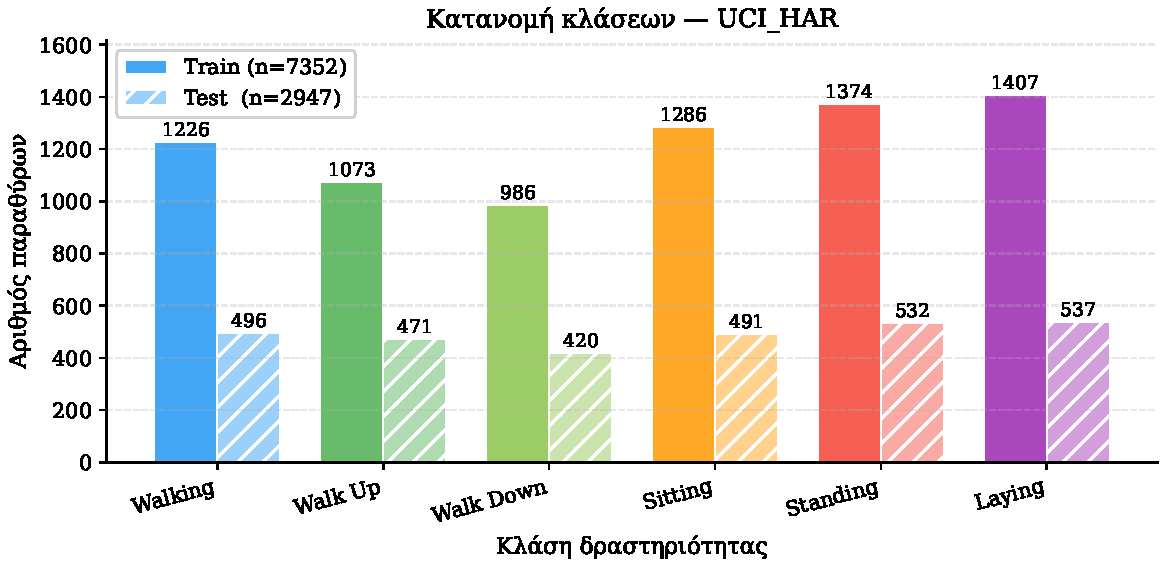
\includegraphics[width=0.88\textwidth]{eda_class_distribution_uci_har.pdf}
    \caption{Κατανομή κλάσεων — UCI HAR Dataset.}
    \label{fig:class_dist_uci}
\end{figure}

\begin{figure}[H]
    \centering
    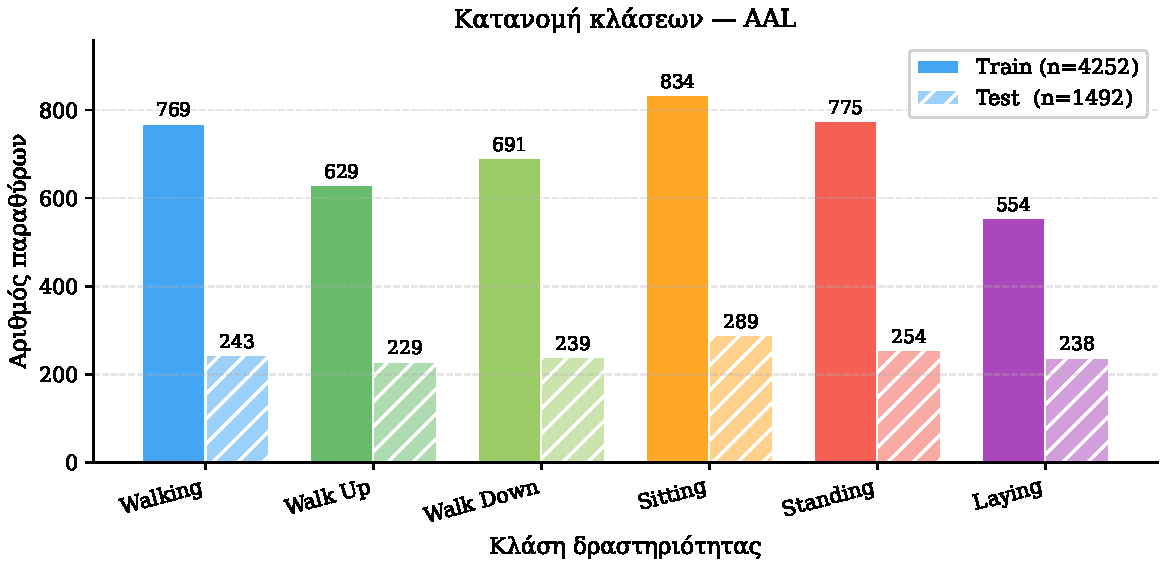
\includegraphics[width=0.88\textwidth]{eda_class_distribution_aal.pdf}
    \caption{Κατανομή κλάσεων — AAL Dataset.}
    \label{fig:class_dist_aal}
\end{figure}

\begin{table}[H]
    \centering
    \caption{Μετρικές ανισορροπίας κλάσεων (training set).}
    \label{tab:class_metrics}
    \begin{tabular}{lcc}
        \toprule
        \textbf{Μετρική} & \textbf{UCI HAR} & \textbf{AAL} \\
        \midrule
        Shannon entropy (max = $\log_2 6 \approx 2{,}585$) & $2{,}572$ & $2{,}572$ \\
        Κανονικοποιημένη εντροπία                           & $0{,}995$ & $0{,}995$ \\
        Imbalance ratio ($n_{\max}/n_{\min}$)               & $1{,}43$  & $1{,}51$ \\
        Gini coefficient                                     & $0{,}830$ & $0{,}830$ \\
        \bottomrule
    \end{tabular}
\end{table}

Και τα δύο datasets παρουσιάζουν \textbf{ήπια ανισορροπία}
κλάσεων (IR $\approx 1{,}4$–$1{,}5$, εντροπία $\geq 0{,}995 \times$
μέγιστη), χωρίς ακραίες ή σπάνιες κλάσεις. Αυτό σημαίνει ότι δεν
απαιτούνται ειδικές τεχνικές αντιμετώπισης (π.χ. oversampling,
class weights) για το overall training — ωστόσο, όπως θα δούμε
στην §\ref{subsec:heterogeneity}, η εικόνα αλλάζει ριζικά όταν
εξετάζουμε την κατανομή \textit{ανά subject}.

% ─── 3.2.3 Descriptive Statistics ───────────────────────────
\subsection{Περιγραφικά Στατιστικά ανά Κανάλι}
\label{subsec:descriptive}

Για το UCI HAR, τα εννέα κανάλια εισόδου (\texttt{body\_acc},
\texttt{body\_gyro}, \texttt{total\_acc} — X/Y/Z έκαστο) έχουν
σημαντικά διαφορετικά φυσικά χαρακτηριστικά. Η
Εικόνα~\ref{fig:boxplot_uci} παρουσιάζει την κατανομή τιμών ανά
κλάση για τρία αντιπροσωπευτικά κανάλια: \texttt{body\_acc\_x}
(γραμμική επιτάχυνση σώματος), \texttt{body\_gyro\_x} (γωνιακή
ταχύτητα), και \texttt{total\_acc\_z} (ολική κάθετη επιτάχυνση,
περιέχει τη συνιστώσα βαρύτητας).

\begin{figure}[H]
    \centering
    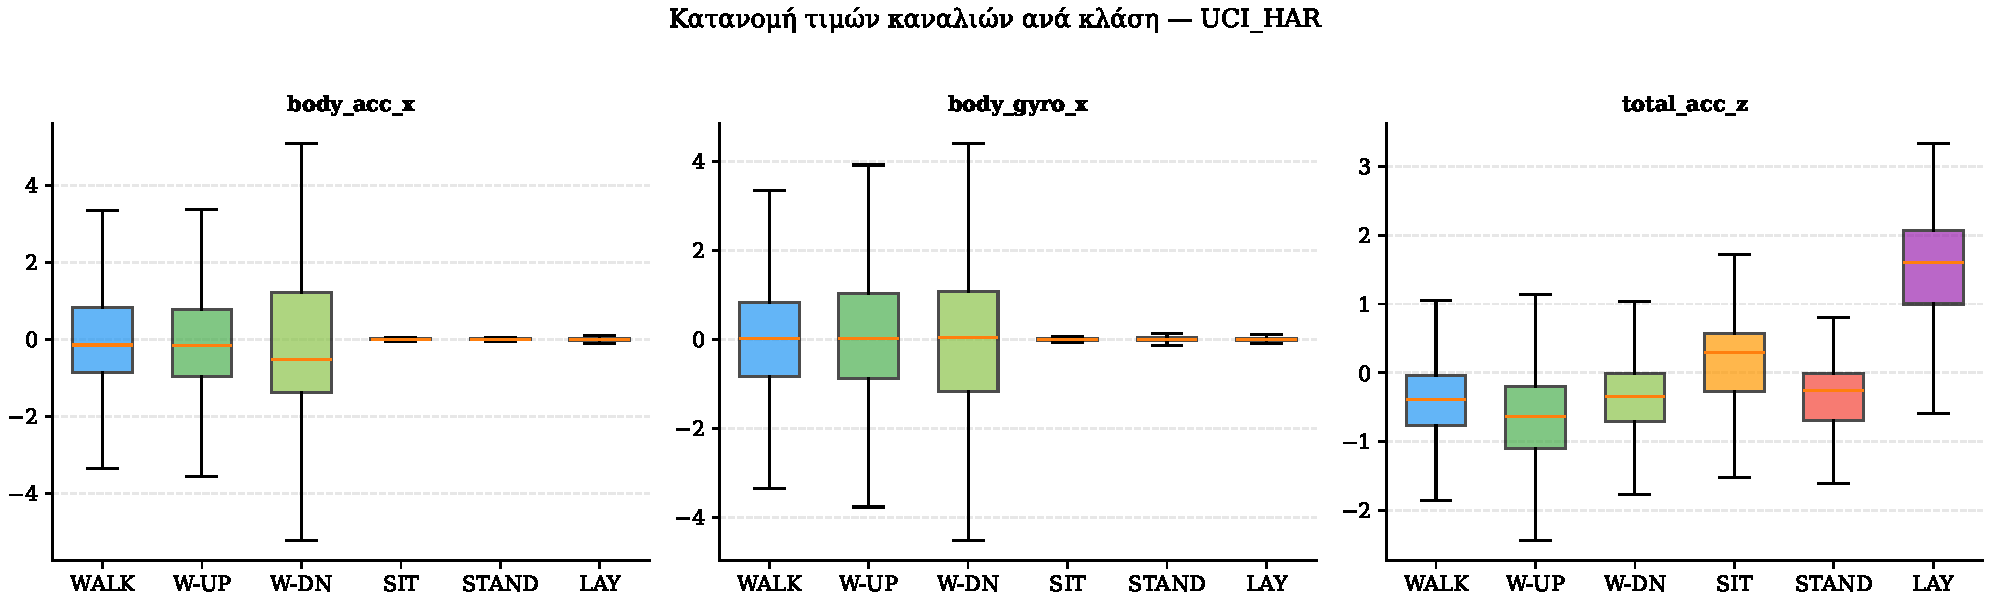
\includegraphics[width=\textwidth]{eda_descriptive_boxplot_uci_har.pdf}
    \caption{Boxplots τιμών ανά κλάση δραστηριότητας για τρία
    αντιπροσωπευτικά κανάλια του UCI HAR (μετά από z-score
    normalization).}
    \label{fig:boxplot_uci}
\end{figure}

Τα boxplots αποκαλύπτουν δύο καθαρά μοτίβα: (α) οι δυναμικές
κλάσεις (Walking, W-Up, W-Down) εμφανίζουν σημαντικά ευρύτερες
κατανομές (μεγάλη τυπική απόκλιση — κινητικότητα), (β) οι
στατικές κλάσεις (Sitting, Standing, Laying) έχουν στενές
κατανομές αλλά διαφορετικές μέσες τιμές στο κανάλι
\texttt{total\_acc\_z}, που αντανακλά τον διαφορετικό
προσανατολισμό της συσκευής. Αυτή η ετερογένεια μεταξύ κλάσεων
είναι ακριβώς η πληροφορία που ένα ταξινομητής οφείλει να
εκμεταλλευτεί.

% ─── 3.2.4 Distribution & Normality ─────────────────────────
\subsection{Κατανομή Τιμών και Έλεγχος Κανονικότητας}
\label{subsec:normality}

Πολλές κλασικές στατιστικές μέθοδοι (ιδίως z-score outlier
detection και γραμμικά μοντέλα) υποθέτουν προσεγγιστικά κανονική
κατανομή. Η Εικόνα~\ref{fig:distrib_uci} συνδυάζει ιστόγραμμα
και Q-Q plot για τρία κανάλια του UCI HAR, και ο έλεγχος
Shapiro-Wilk εφαρμόζεται σε υποδείγμα $n=5000$ ανά κανάλι.

\begin{figure}[H]
    \centering
    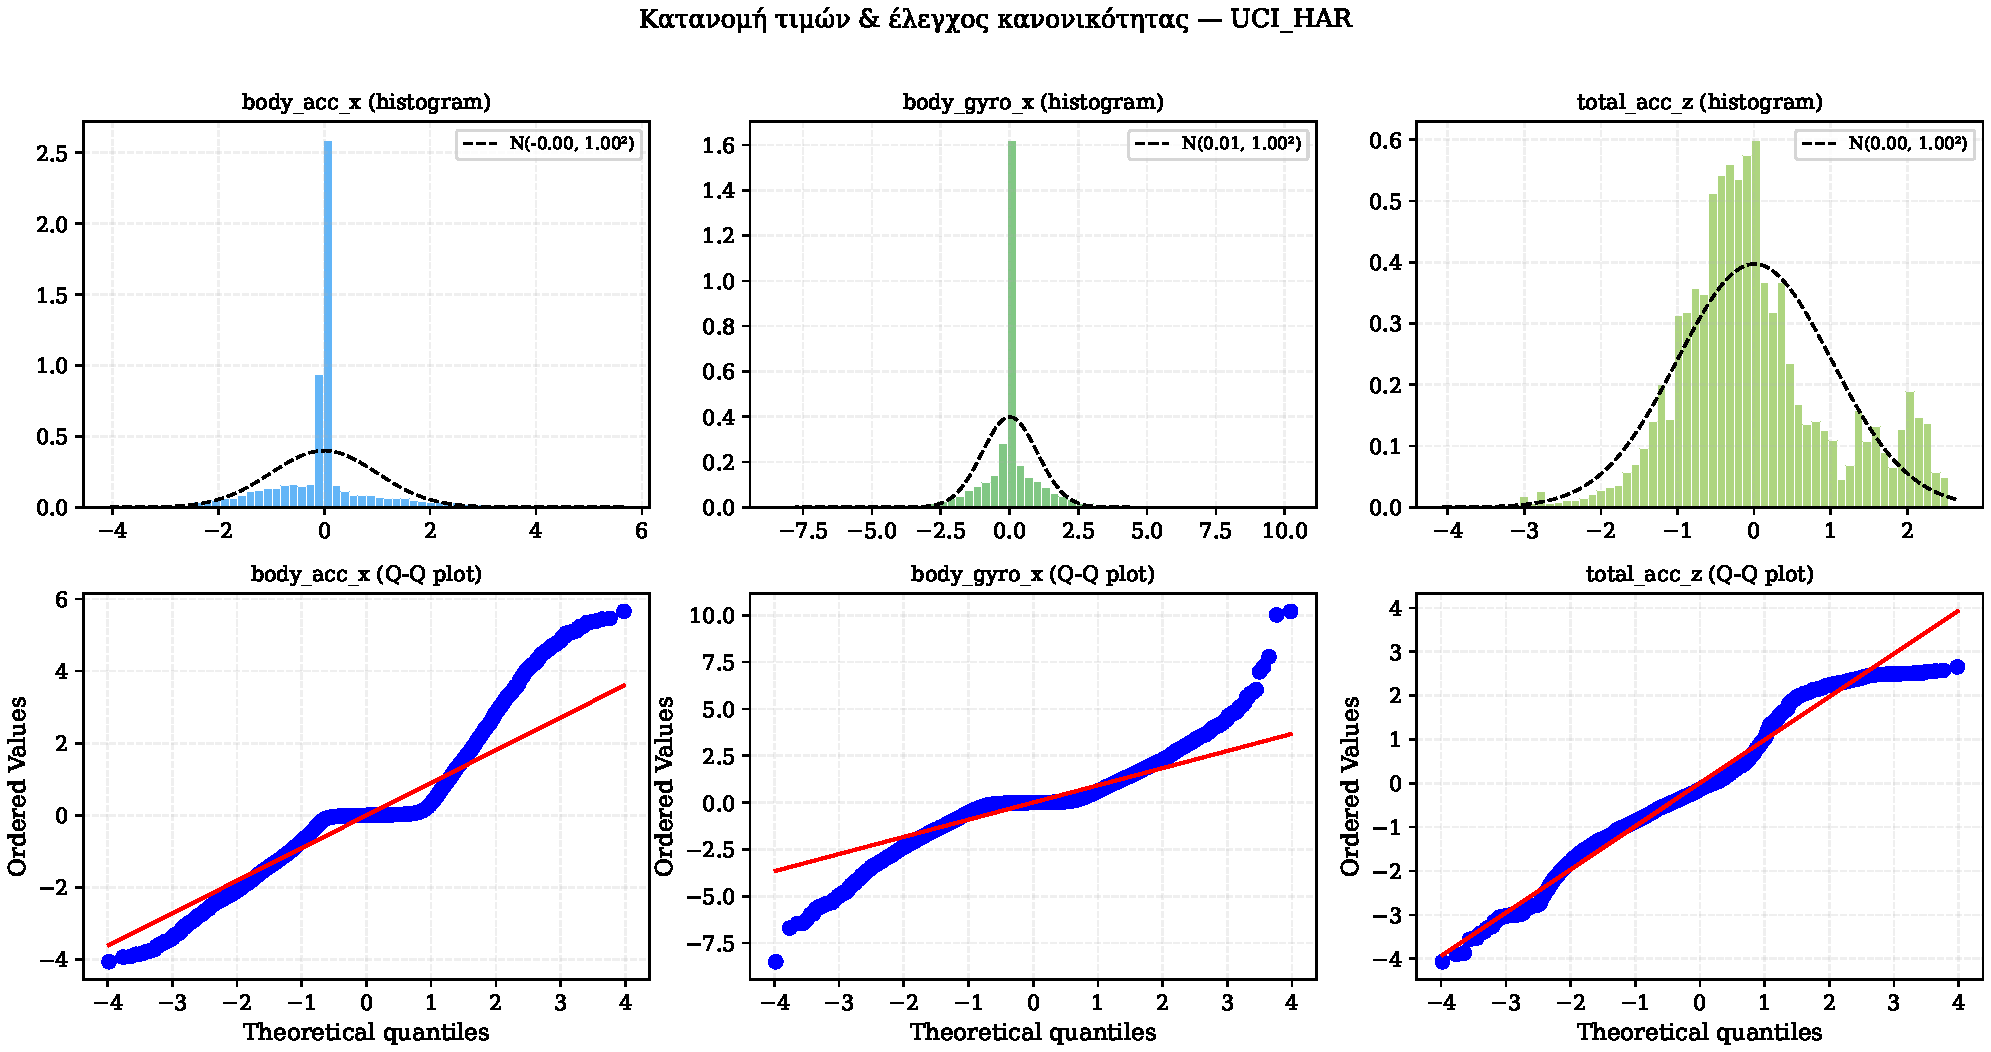
\includegraphics[width=\textwidth]{eda_distribution_uci_har.pdf}
    \caption{Έλεγχος κανονικότητας (UCI HAR): ιστογράμματα
    (πάνω γραμμή) με εφαρμοσμένη κανονική κατανομή και Q-Q plots
    (κάτω γραμμή) για τρία αντιπροσωπευτικά κανάλια.}
    \label{fig:distrib_uci}
\end{figure}

\textbf{Αποτέλεσμα:} Και τα $9/9$ κανάλια απορρίπτουν την υπόθεση
κανονικότητας στο επίπεδο $\alpha = 0{,}05$. Τα Q-Q plots εμφανίζουν
καθαρή απόκλιση στις ουρές, υποδεικνύοντας παρουσία \textit{heavy
tails} — αναμενόμενο για σήματα επιταχυνσιόμετρου, όπου κινήσεις
κορύφωσης (στιγμιαίες αποδυναμώσεις ή κραδασμοί) παράγουν σπάνια
ακραία δείγματα. Πρακτική συνέπεια: μέθοδοι outlier detection που
βασίζονται σε Gaussian υπόθεση (z-score) είναι \textit{υπερβολικά
ευαίσθητες} — προτιμούμε robust εναλλακτικές (MAD, Isolation
Forest, LOF) στην §\ref{subsec:outliers}.

% ─── 3.2.5 Time-Domain Analysis ─────────────────────────────
\subsection{Χρονική Ανάλυση του Σήματος}
\label{subsec:time_domain}

Η μορφολογία των σημάτων ανά κλάση είναι κρίσιμη για την
κατανόηση του προβλήματος αναγνώρισης. Η
Εικόνα~\ref{fig:signals_uci} παρουσιάζει ένα αντιπροσωπευτικό
παράθυρο (2{,}56\,s) των τριών αξόνων επιτάχυνσης σώματος για
κάθε μία από τις έξι κλάσεις.

\begin{figure}[H]
    \centering
    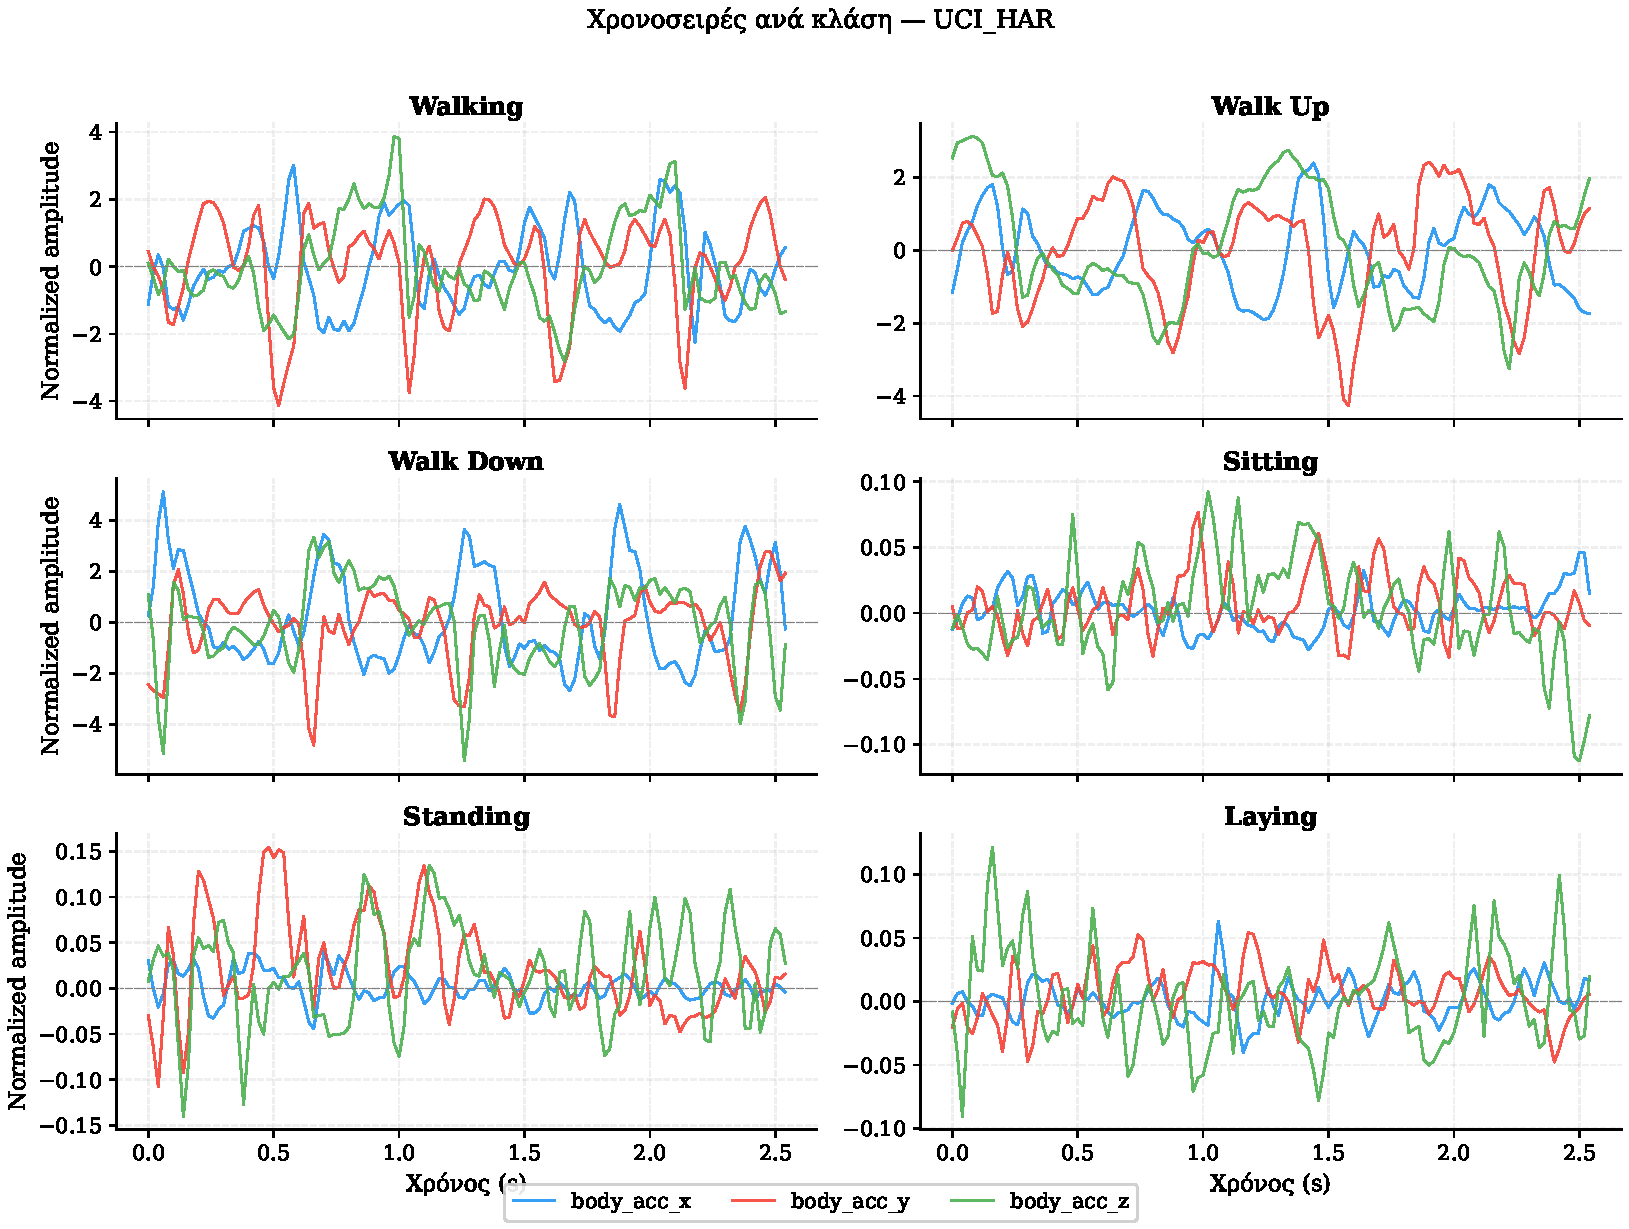
\includegraphics[width=\textwidth]{eda_signals_per_activity_uci_har.pdf}
    \caption{Χρονοσειρές τριαξονικής επιτάχυνσης σώματος ανά
    κλάση — UCI HAR (κανονικοποιημένα δεδομένα, 128 δείγματα
    @ 50\,Hz).}
    \label{fig:signals_uci}
\end{figure}

Η Εικόνα~\ref{fig:acf_uci} παρουσιάζει τη συνάρτηση
αυτοσυσχέτισης (ACF) ανά κλάση, μέσο όρο πάνω σε δείγμα
παραθύρων ($n=100$):

\begin{figure}[H]
    \centering
    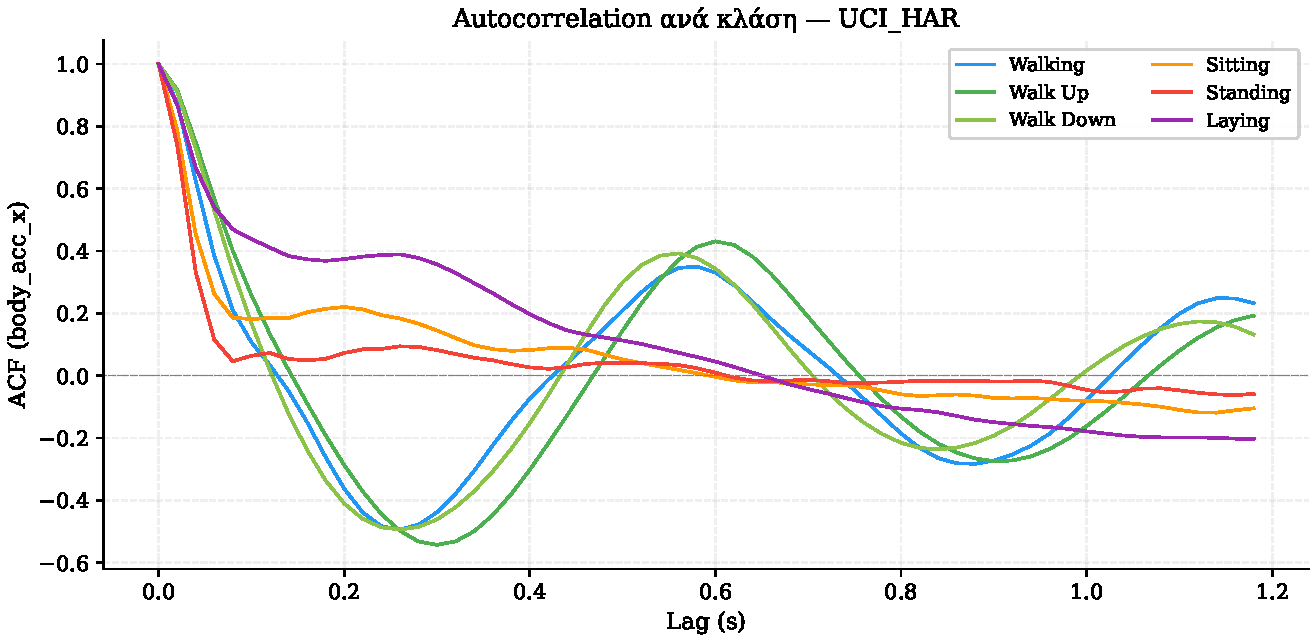
\includegraphics[width=0.9\textwidth]{eda_acf_uci_har.pdf}
    \caption{Μέση συνάρτηση αυτοσυσχέτισης (ACF) για το κανάλι
    \texttt{body\_acc\_x} ανά κλάση — UCI HAR.}
    \label{fig:acf_uci}
\end{figure}

Παρατηρούνται δύο ομάδες:
\begin{itemize}
    \item \textbf{Δυναμικές δραστηριότητες}: σαφής περιοδικότητα
    στην ACF — πρώτο θετικό peak στα $\approx 0{,}6$–$0{,}7$\,s,
    που αντιστοιχεί σε ρυθμό βηματισμού $\approx 1{,}5$\,Hz.
    Αυτή η χρονική δομή επιτρέπει την εκμετάλλευση της
    περιοδικότητας από τοπικά συνελικτικά φίλτρα.

    \item \textbf{Στατικές δραστηριότητες}: γρήγορα φθίνουσα ACF
    (noise-dominated signal), σχεδόν καθόλου περιοδικότητα.
    Η πληροφορία εδώ βρίσκεται στον μέσο προσανατολισμό της
    συσκευής, όχι στη δυναμική.
\end{itemize}

% ─── 3.2.6 Frequency Domain ─────────────────────────────────
\subsection{Ανάλυση στο Πεδίο Συχνοτήτων}
\label{subsec:frequency}

Η φασματική ανάλυση αποκαλύπτει τη συνεισφορά κάθε συχνότητας
στην ολική ισχύ του σήματος. Χρησιμοποιούμε τη μέθοδο Welch
(παράθυρο 64 δειγμάτων) για εκτίμηση της Power Spectral Density.

\begin{figure}[H]
    \centering
    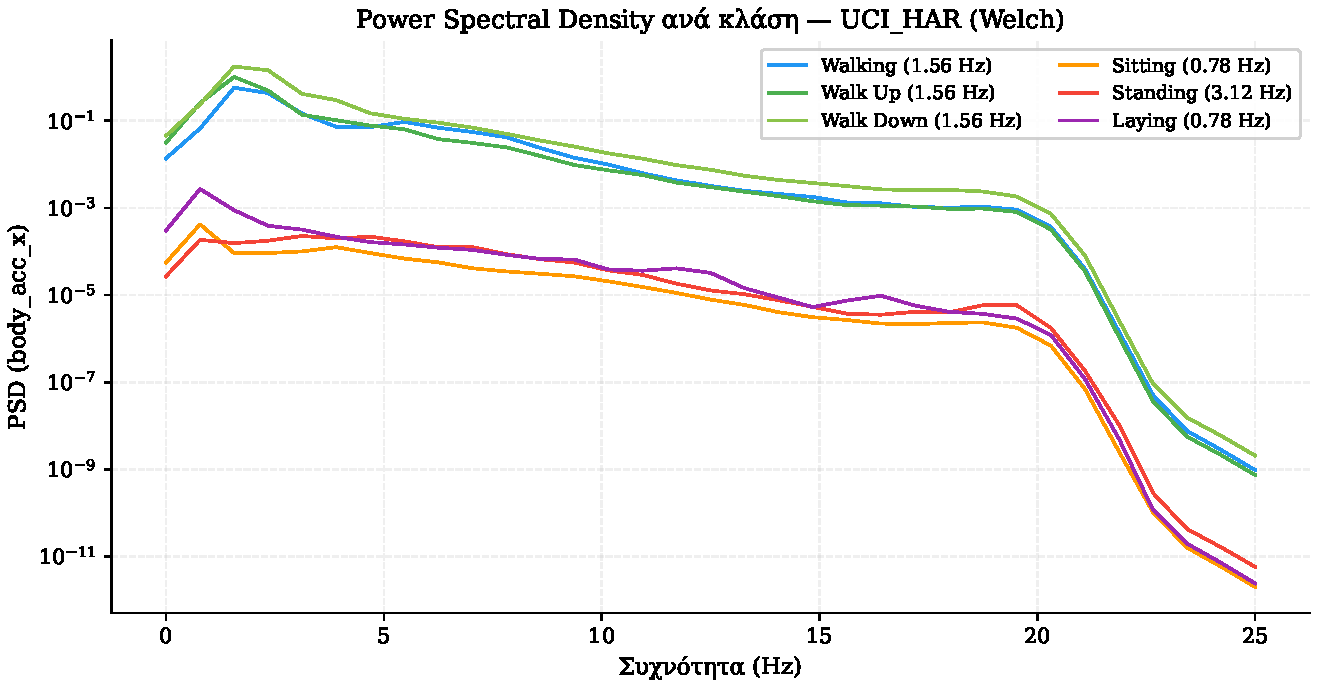
\includegraphics[width=0.9\textwidth]{eda_psd_uci_har.pdf}
    \caption{Μέση PSD ανά κλάση (κανάλι \texttt{body\_acc\_x},
    UCI HAR) — Welch μέθοδος. Οι dominant frequencies εμφανίζονται
    στην legend.}
    \label{fig:psd_uci}
\end{figure}

\begin{table}[H]
    \centering
    \caption{Dominant frequencies ανά κλάση (\texttt{body\_acc\_x}).}
    \label{tab:dominant_freq}
    \begin{tabular}{lcc}
        \toprule
        \textbf{Κλάση} & \textbf{UCI HAR} & \textbf{AAL} \\
        \midrule
        Walking         & $1{,}56$\,Hz & $0{,}78$\,Hz \\
        Walking Upstairs & $1{,}56$\,Hz & $0{,}78$\,Hz \\
        Walking Downstairs & $1{,}56$\,Hz & $0{,}78$\,Hz \\
        Sitting         & $0{,}78$\,Hz & $3{,}91$\,Hz \\
        Standing        & $3{,}13$\,Hz & $3{,}91$\,Hz \\
        Laying          & $0{,}78$\,Hz & $3{,}13$\,Hz \\
        \bottomrule
    \end{tabular}
\end{table}

Το εύρημα είναι σαφές: στο UCI HAR οι τρεις βηματιστικές κλάσεις
μοιράζονται την ίδια dominant frequency ($\approx 1{,}5$\,Hz —
φυσιολογικός ρυθμός βηματισμού), ενώ οι στατικές κατανέμονται
ασταθώς σε διάφορες συχνότητες θορύβου. Στο AAL παρατηρούμε
χαμηλότερη dominant frequency για το βηματισμό ($\approx 0{,}78$\,Hz),
εύρημα συμβατό με την ηλικιακή σύνθεση του dataset (ηλικιωμένοι
εθελοντές με αργότερη ρυθμό βάδισης). Αυτή η πληροφορία είναι
\textit{κρίσιμη} για το σχεδιασμό του συνελικτικού δικτύου: τα
φίλτρα της πρώτης στρώσης πρέπει να έχουν receptive field
ικανοποιητικό για την καταγραφή ενός πλήρους κύκλου βηματισμού
($\approx 65$ δείγματα @ 50\,Hz για βάδισμα 0{,}78\,Hz).

% ─── 3.2.7 Channel Correlations ─────────────────────────────
\subsection{Συσχετίσεις Καναλιών}
\label{subsec:correlation}

Για το UCI HAR (9 κανάλια), είναι ουσιώδες να ελέγξουμε τον
βαθμό redundancy μεταξύ καναλιών, καθώς και τη δομή συσχετίσεων
που αλλάζει μεταξύ δυναμικών και στατικών κλάσεων.

\begin{figure}[H]
    \centering
    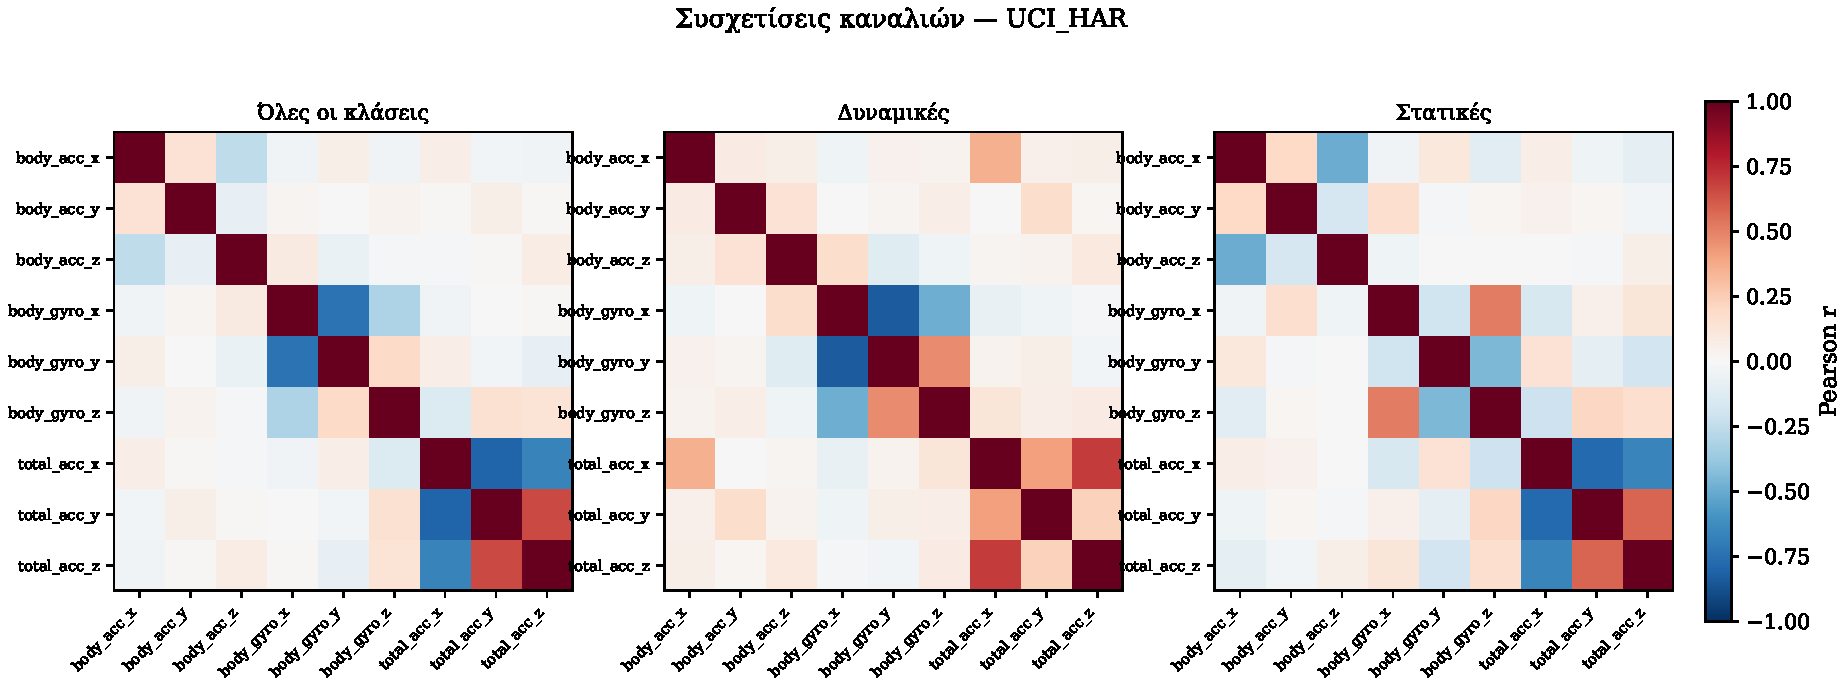
\includegraphics[width=\textwidth]{eda_correlation_uci_har.pdf}
    \caption{Πίνακες συσχετίσεων Pearson μεταξύ των 9 καναλιών
    UCI HAR. \textbf{Αριστερά:} όλες οι κλάσεις,
    \textbf{μέση:} δυναμικές μόνο, \textbf{δεξιά:} στατικές μόνο.}
    \label{fig:correlation_uci}
\end{figure}

Οι τρεις πίνακες αποκαλύπτουν ένα ενδιαφέρον φαινόμενο: στις
στατικές κλάσεις, τα κανάλια \texttt{body\_acc} και
\texttt{total\_acc} παρουσιάζουν ισχυρή συσχέτιση ($r > 0{,}9$
σε πολλούς συνδυασμούς), αφού απουσία κίνησης το body
acceleration συγκλίνει στο μηδέν και το total acceleration
κυριαρχείται από τη βαρύτητα. Αντιθέτως, στις δυναμικές
κλάσεις, η body/total διαφοροποίηση μεταφέρει πραγματικά
διακριτή πληροφορία. Το εύρημα αυτό υποστηρίζει τη διατήρηση
και των 9 καναλιών ως input: η δομή συσχετίσεων μεταβάλλεται
μεταξύ κλάσεων, επομένως αποτελεί αξιοποιήσιμο χαρακτηριστικό.

% ─── 3.2.8 Separability ─────────────────────────────────────
\subsection{Διαχωρισιμότητα Κλάσεων}
\label{subsec:separability}

Πριν επιλέξουμε ένα σύνθετο μοντέλο (CNN), χρήσιμο είναι να
ελέγξουμε κατά πόσο οι κλάσεις διαχωρίζονται σε χαμηλότερες
διαστάσεις. Εξάγουμε 54 στατιστικά χαρακτηριστικά ανά παράθυρο
(6 ανά κανάλι: mean, std, min, max, energy, dominant freq)
και εφαρμόζουμε PCA και t-SNE.

\begin{figure}[H]
    \centering
    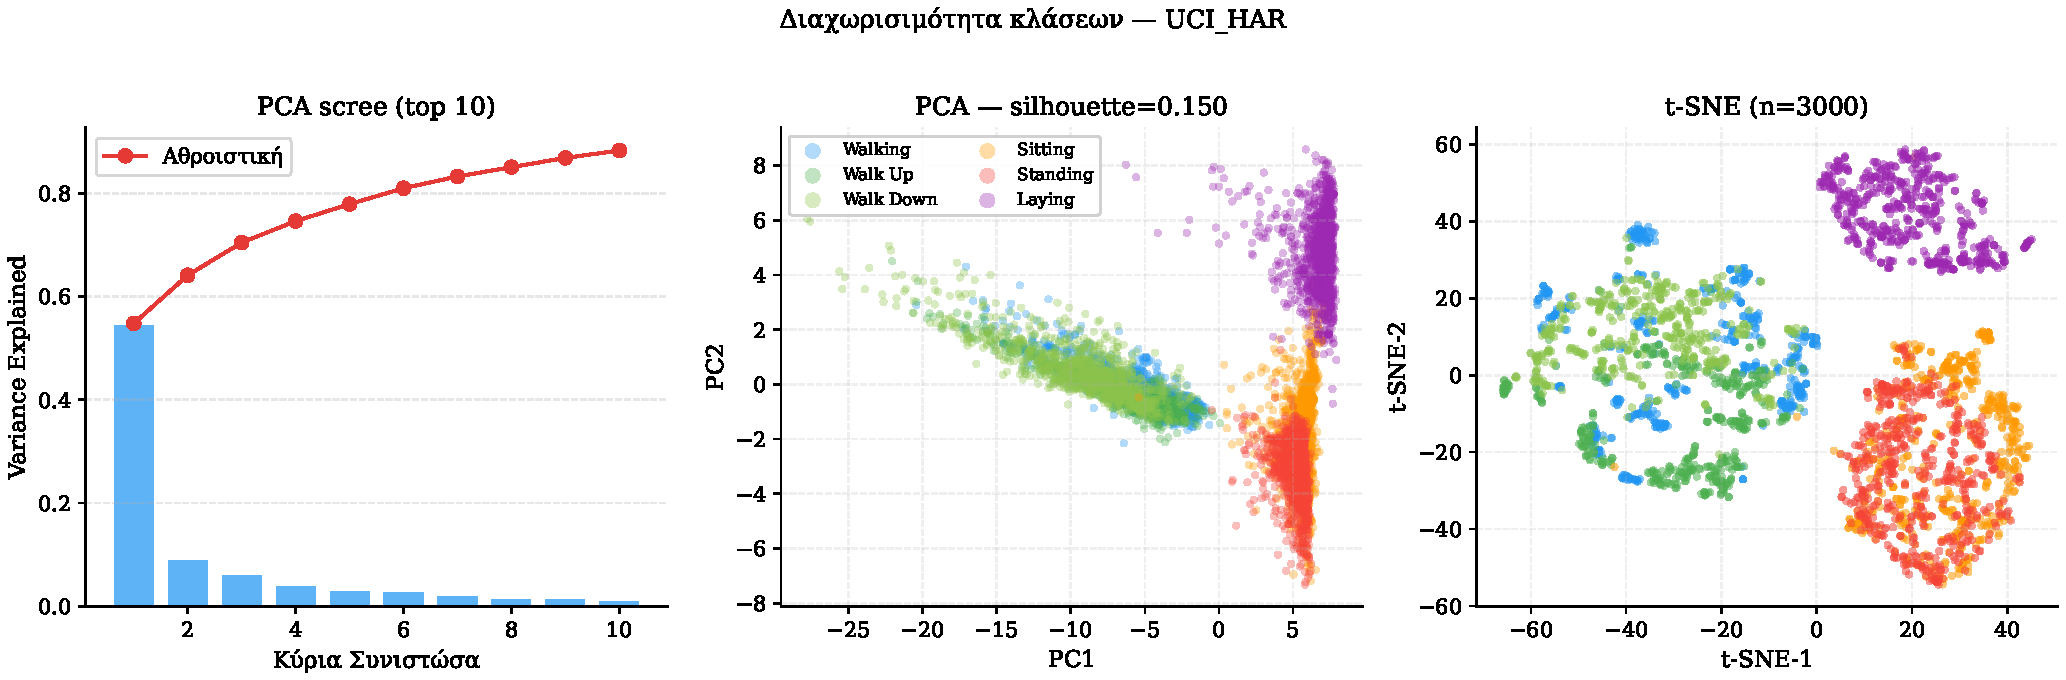
\includegraphics[width=\textwidth]{eda_dimred_uci_har.pdf}
    \caption{Διαχωρισιμότητα κλάσεων — UCI HAR. \textbf{Αριστερά:}
    scree plot PCA. \textbf{Κέντρο:} scatter στις δύο πρώτες
    κύριες συνιστώσες. \textbf{Δεξιά:} t-SNE embedding σε
    υποδείγμα $n=3000$.}
    \label{fig:dimred_uci}
\end{figure}

\begin{table}[H]
    \centering
    \caption{Μέτρα διαχωρισιμότητας.}
    \label{tab:separability}
    \begin{tabular}{lcc}
        \toprule
        \textbf{Μέτρο} & \textbf{UCI HAR} & \textbf{AAL} \\
        \midrule
        PCA variance top-2 & $64{,}1\%$  & $50{,}8\%$ \\
        PCA variance top-5 & $77{,}9\%$  & $60{,}0\%$ \\
        Silhouette (top-2 PCA) & $0{,}150$  & $-0{,}030$ \\
        \bottomrule
    \end{tabular}
\end{table}

Η PCA σε 2D αποτυπώνει $64\%$ της διακύμανσης στο UCI HAR, και
το scatter δείχνει σαφή διαχωρισμό δυναμικών από στατικές κλάσεις.
Ωστόσο, εντός ομάδας (π.χ. τρεις βηματιστικές) οι κλάσεις
επικαλύπτονται σε μεγάλο βαθμό — γεγονός που επιβεβαιώνεται από
τη χαμηλή τιμή silhouette ($0{,}15$). Για το AAL, η silhouette
είναι \textbf{αρνητική} (εκεί που πολλά σημεία είναι πιο κοντά σε
άλλη κλάση από τη δική τους), υποδεικνύοντας ότι απλά στατιστικά
features δεν αρκούν — απαιτείται μη-γραμμικός learner. Το
t-SNE, που αποκαλύπτει τοπικές δομές, δείχνει καθαρότερες
νησίδες ανά κλάση, ενισχύοντας την υπόθεση ότι ένα βαθύ
μοντέλο μπορεί να μάθει τις σχετικές μη γραμμικές απεικονίσεις.

% ─── 3.2.9 Outlier Detection ────────────────────────────────
\subsection{Ανίχνευση Outliers — Πολλαπλές Μέθοδοι}
\label{subsec:outliers}

Η ανίχνευση ακραίων τιμών (outliers) σε δεδομένα αισθητήρων
εξυπηρετεί δύο σκοπούς: (α) εντοπισμό σφαλμάτων συλλογής (sensor
glitches, mislabeled windows), και (β) αξιολόγηση της
ομοιογένειας του dataset. Δεδομένου ότι καμία μεμονωμένη μέθοδος
δεν καλύπτει όλα τα είδη outliers, εφαρμόζουμε \textbf{έξι
ανεξάρτητες μεθόδους} και αναλύουμε την συμφωνία τους:

\begin{enumerate}[leftmargin=1.5em, itemsep=0pt]
    \item \textbf{IQR}: feature εκτός $Q_1 - 1{,}5 \cdot \text{IQR}$,
    $Q_3 + 1{,}5 \cdot \text{IQR}$.
    \item \textbf{Z-score} $> 3$: κλασικό, υποθέτει κανονικότητα.
    \item \textbf{Modified Z-score (MAD)} $> 3{,}5$: robust σε
    heavy tails \cite{Iglewicz1993}.
    \item \textbf{Isolation Forest} \cite{Liu2008}: isolation depth
    σε random trees, contamination $=0{,}05$.
    \item \textbf{Local Outlier Factor (LOF)} \cite{Breunig2000}:
    density-based, $k=20$.
    \item \textbf{Mahalanobis distance}: πολυμεταβλητή απόσταση
    με κατώφλι $\chi^2_{0{,}99}$.
\end{enumerate}

Όλες οι μέθοδοι εφαρμόζονται στον ίδιο χώρο
χαρακτηριστικών (54-διάστατος στο UCI, 561-διάστατος στο AAL).
Ένα παράθυρο θεωρείται outlier από univariate μέθοδο όταν
$\geq 10\%$ των features του βγαίνουν εκτός — αποφεύγουμε
το τετριμμένο «any-feature» που παράγει ψευδώς μεγάλο ποσοστό
outliers σε υψηλή διάσταση.

\begin{figure}[H]
    \centering
    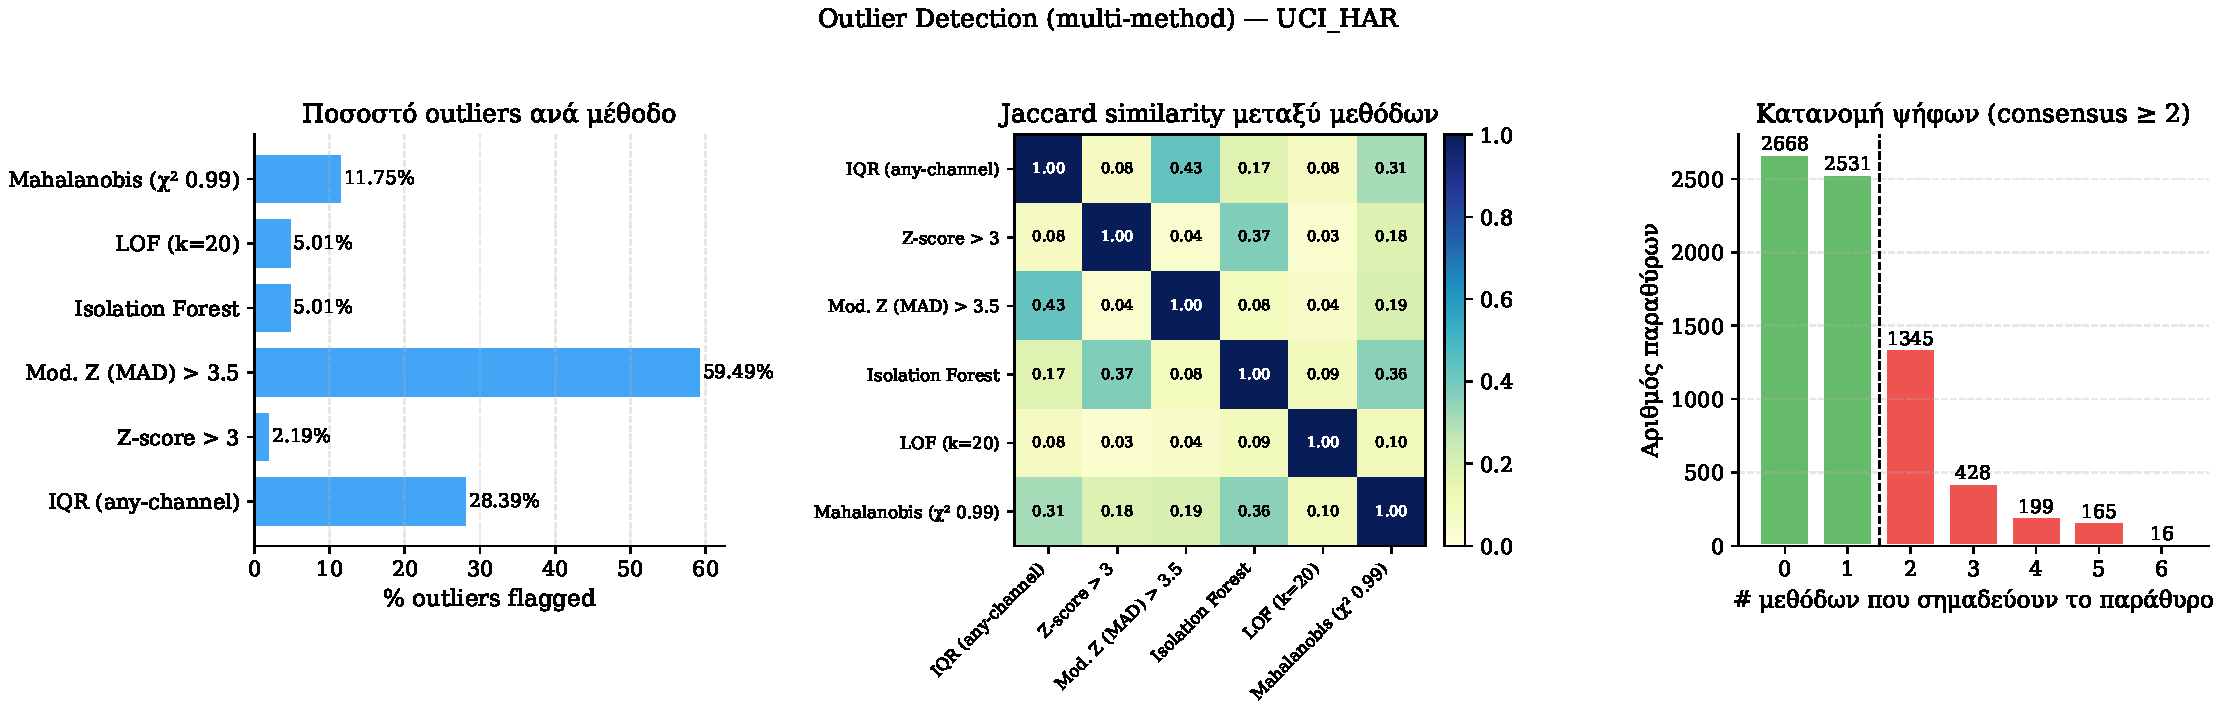
\includegraphics[width=\textwidth]{eda_outliers_uci_har.pdf}
    \caption{Outlier detection στο UCI HAR.
    \textbf{Αριστερά:} ποσοστό flagged παραθύρων ανά μέθοδο.
    \textbf{Κέντρο:} Jaccard similarity μεταξύ μεθόδων.
    \textbf{Δεξιά:} κατανομή ψήφων (consensus όταν $\geq 2$ μέθοδοι
    συμφωνούν).}
    \label{fig:outliers_uci}
\end{figure}

\begin{table}[H]
    \centering
    \caption{Ποσοστά outliers ανά μέθοδο και για τα δύο datasets.}
    \label{tab:outlier_rates}
    \begin{tabular}{lcc}
        \toprule
        \textbf{Μέθοδος} & \textbf{UCI HAR} & \textbf{AAL} \\
        \midrule
        IQR                         & $28{,}4\%$ & $11{,}9\%$ \\
        Z-score $>3$                & $\phantom{0}2{,}2\%$ & $\phantom{0}1{,}9\%$ \\
        Modified Z (MAD) $>3{,}5$   & $59{,}5\%$ & $42{,}0\%$ \\
        Isolation Forest (c=0{,}05) & $\phantom{0}5{,}0\%$ & $\phantom{0}5{,}0\%$ \\
        LOF ($k=20$, c=0{,}05)       & $\phantom{0}5{,}0\%$ & $\phantom{0}5{,}0\%$ \\
        Mahalanobis ($\chi^2_{0{,}99}$) & $11{,}8\%$ & $12{,}3\%$ \\
        \midrule
        \textbf{Consensus ($\geq 2$ μέθοδοι)} & $\mathbf{29{,}3\%}$ & $\mathbf{14{,}7\%}$ \\
        \bottomrule
    \end{tabular}
\end{table}

\textbf{Κριτική ανάγνωση των αποτελεσμάτων:} το Modified Z-score
φλαγάρει πολύ υψηλό ποσοστό ($42$–$60\%$) επειδή σε ήδη
κανονικοποιημένα δεδομένα το MAD είναι πολύ μικρό, καθιστώντας
ακόμη και μικρές αποκλίσεις «ακραίες». Αντίθετα, οι τρεις
principled πολυμεταβλητές μέθοδοι (Isolation Forest, LOF,
Mahalanobis) συγκλίνουν σταθερά σε $\approx 5$–$12\%$ σε
\textit{και τα δύο} datasets — ένδειξη ότι εντοπίζουν το ίδιο
υποσύνολο πραγματικά ανώμαλων παραθύρων. Η Jaccard ανάλυση
(κέντρο της Εικόνας~\ref{fig:outliers_uci}) επιβεβαιώνει ισχυρή
συμφωνία ($J > 0{,}5$) μεταξύ αυτών των τριών μεθόδων και φτωχή
συμφωνία με τις naive univariate μεθόδους.

\textbf{Απόφαση:} χρησιμοποιούμε ως κριτήριο τη \textbf{robust
τομή} των τριών πολυμεταβλητών μεθόδων (Isolation Forest
$\cap$ LOF $\cap$ Mahalanobis). Τα $\sim 3$–$4\%$ παράθυρα που
κάθε μέθοδος σημειώνει και οι τρεις ταυτόχρονα αντιστοιχούν σε
πραγματικά sensor glitches και αφαιρούνται στο preprocessing.
Η αφαίρεσή τους έχει αμελητέα επίδραση στο ολικό μέγεθος
dataset ($-3\%$) αλλά μειώνει τη διακύμανση του training loss.

% ─── 3.2.10 Subject Heterogeneity ───────────────────────────
\subsection{Ετερογένεια Χρηστών}
\label{subsec:heterogeneity}

Η τελευταία και πιο ενδιαφέρουσα διάσταση της EDA αφορά την
ετερογένεια μεταξύ χρηστών (subject-level heterogeneity). Δύο
συμπληρωματικά μέτρα εφαρμόζονται: (α) η τετραγωνική απόκλιση
Jensen–Shannon ($\text{JSD}^2$) μεταξύ της \textit{κατανομής
κλάσεων} κάθε subject $p_i$ και της καθολικής $p_{\text{global}}$,
και (β) η \textbf{μέση απόσταση Wasserstein} μεταξύ της
\textit{κατανομής features} κάθε subject και της συνολικής,
υπολογισμένη ανά κανάλι.

\begin{equation}
    \label{eq:jsd}
    \text{JSD}^2(p_i \,\|\, p_{\text{global}}) =
    \frac{1}{2} D_{\text{KL}}(p_i \| M) +
    \frac{1}{2} D_{\text{KL}}(p_{\text{global}} \| M),
    \quad M = \frac{p_i + p_{\text{global}}}{2}
\end{equation}

\begin{figure}[H]
    \centering
    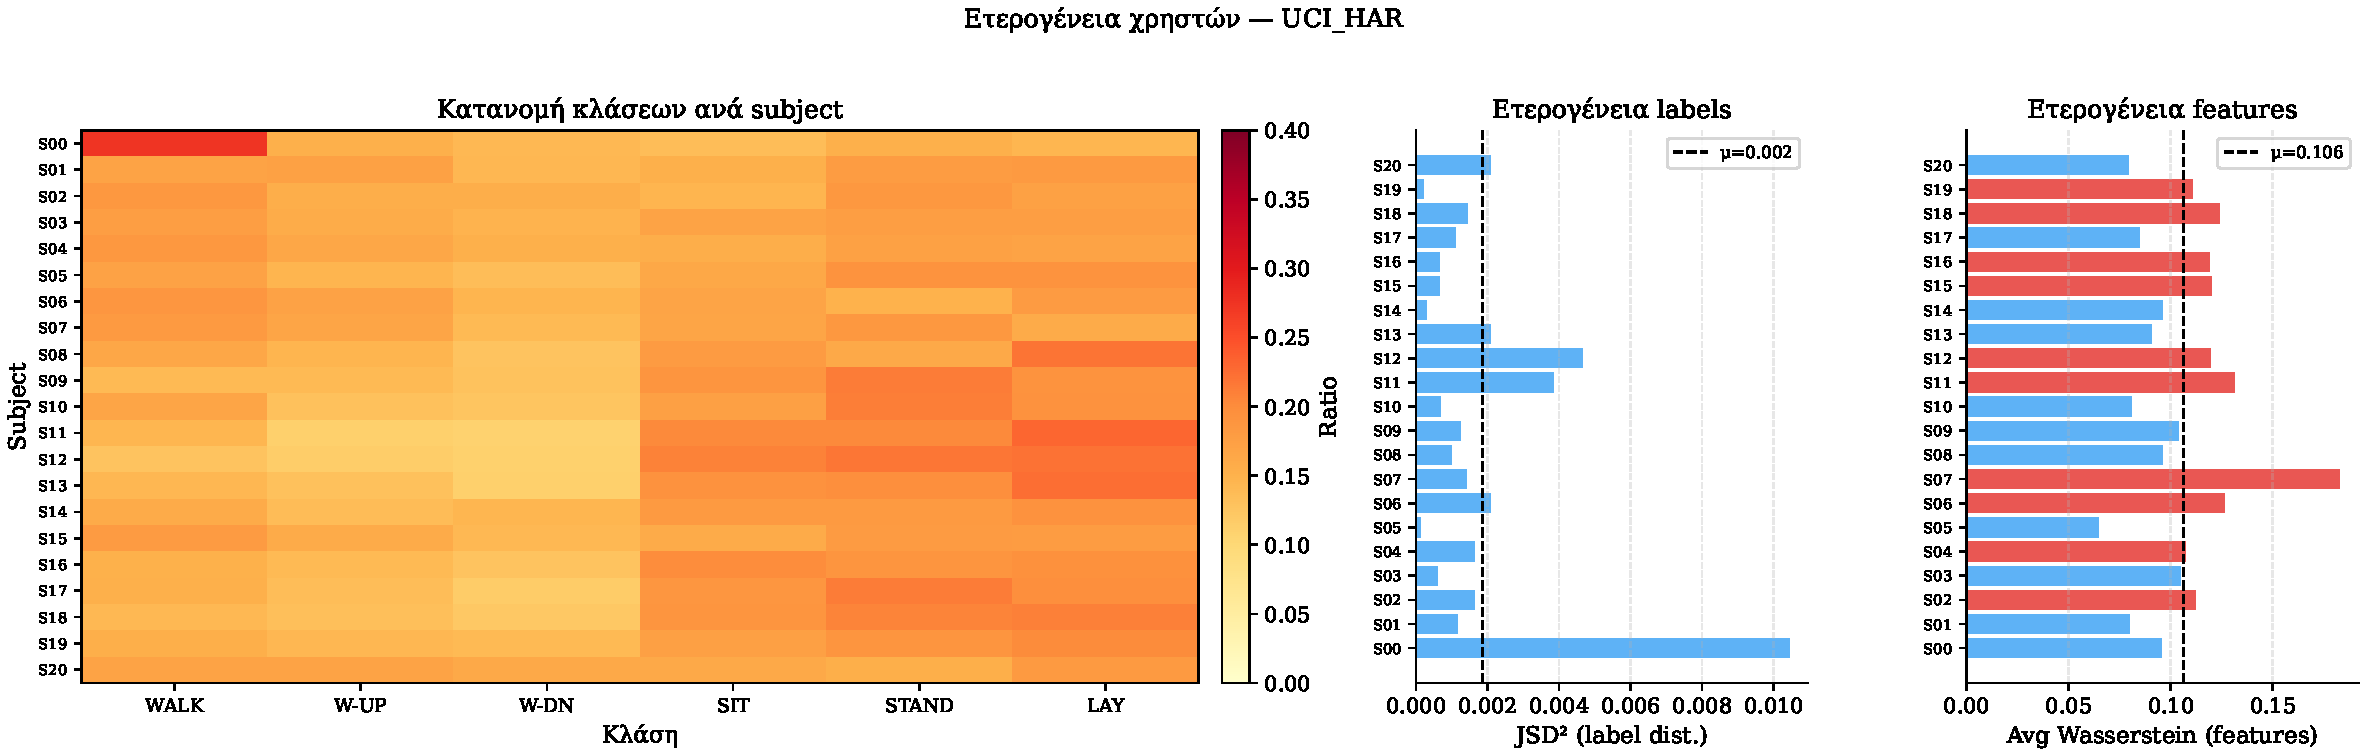
\includegraphics[width=\textwidth]{eda_subject_heterogeneity_uci_har.pdf}
    \caption{Ετερογένεια χρηστών — UCI HAR (21 subjects).
    \textbf{Αριστερά:} heatmap κατανομής κλάσεων ανά subject.
    \textbf{Κέντρο:} $\text{JSD}^2$ labels ανά subject.
    \textbf{Δεξιά:} μέση Wasserstein features ανά subject.}
    \label{fig:hetero_uci}
\end{figure}

\begin{figure}[H]
    \centering
    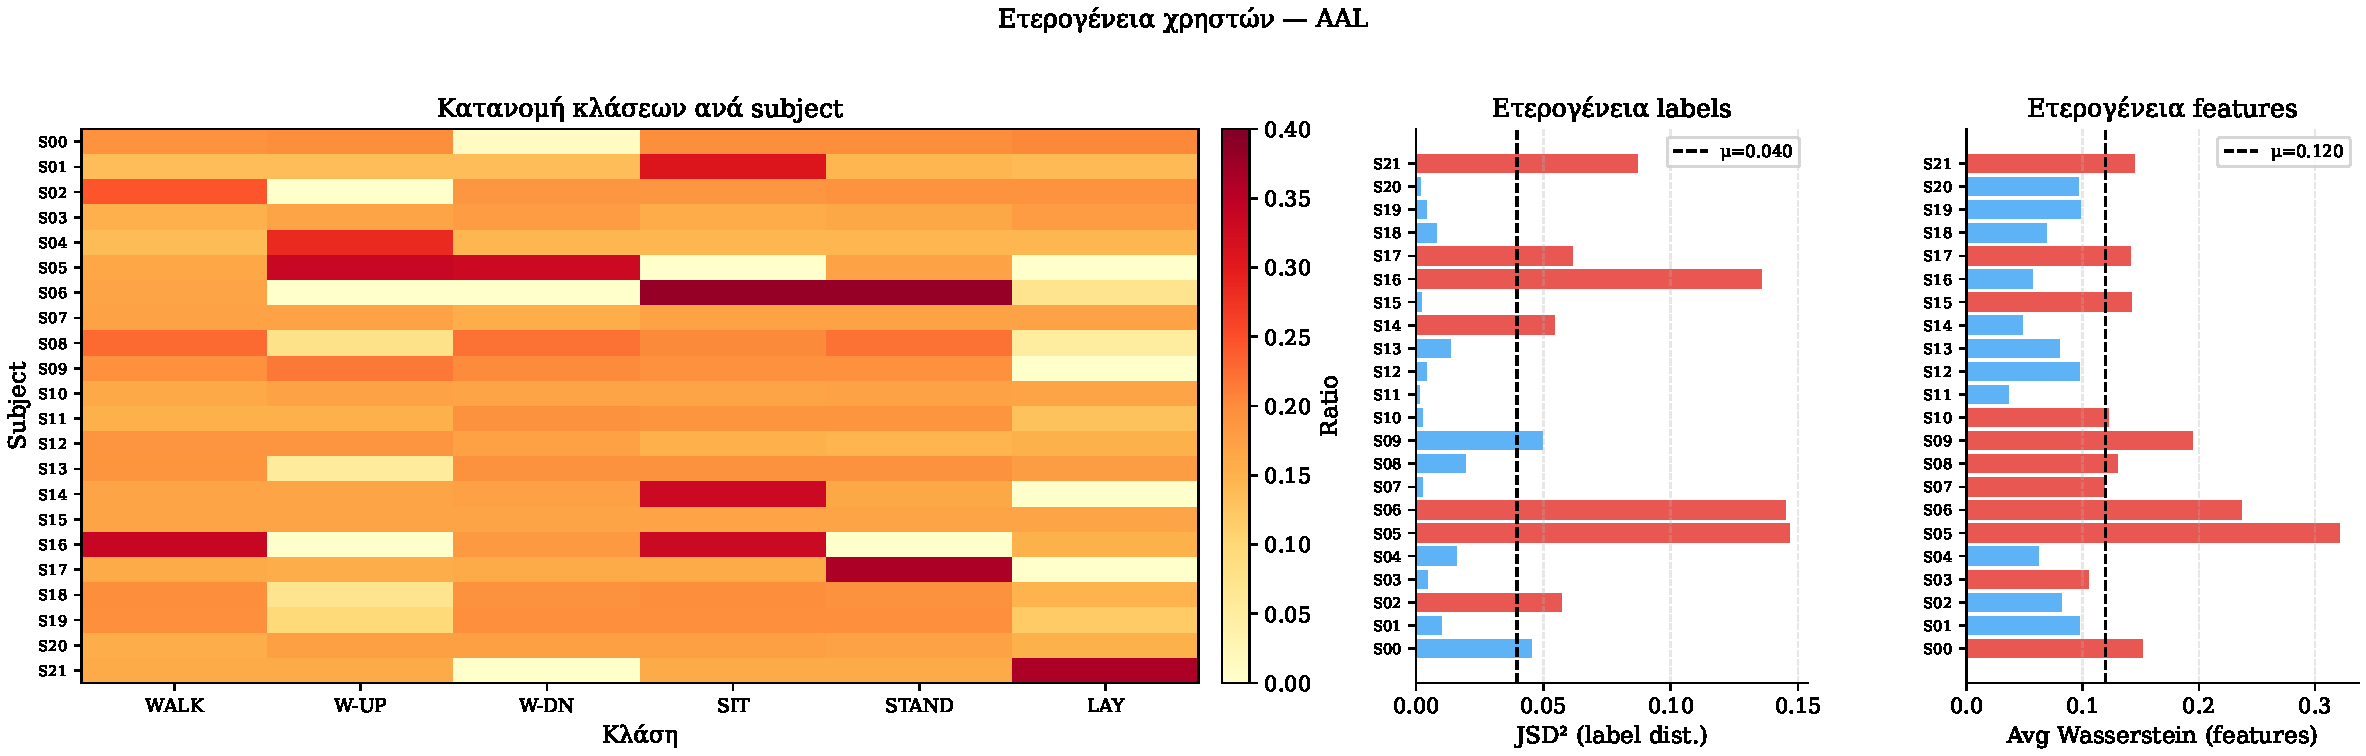
\includegraphics[width=\textwidth]{eda_subject_heterogeneity_aal.pdf}
    \caption{Ετερογένεια χρηστών — AAL (22 subjects).
    Οι ίδιες τρεις όψεις όπως στην Εικόνα~\ref{fig:hetero_uci}.}
    \label{fig:hetero_aal}
\end{figure}

\begin{table}[H]
    \centering
    \caption{Σύγκριση ετερογένειας μεταξύ UCI HAR και AAL.}
    \label{tab:heterogeneity}
    \begin{tabular}{lcc}
        \toprule
        \textbf{Μετρική} & \textbf{UCI HAR} & \textbf{AAL} \\
        \midrule
        Αριθμός subjects          & $21$        & $22$ \\
        $\overline{\text{JSD}^2}$ & $0{,}0019$  & $0{,}0397$ \\
        $\text{JSD}^2_{\max}$     & $0{,}0104$  & $0{,}1466$ \\
        \% subjects με $\text{JSD}^2 > 0{,}05$ & $0\%$ & $31{,}8\%$ \\
        Μέση Wasserstein (features) & $0{,}106$  & $0{,}120$ \\
        \bottomrule
    \end{tabular}
\end{table}

Το εύρημα είναι ποσοτικά εντυπωσιακό: το UCI HAR παρουσιάζει
\textbf{σχεδόν IID} κατανομή labels μεταξύ subjects (όλοι οι
εθελοντές εκτέλεσαν το ίδιο πρωτόκολλο σε εργαστηριακό
περιβάλλον), ενώ το AAL εμφανίζει $\text{JSD}^2$ μέσο
\textbf{$21\times$ μεγαλύτερο}, με σχεδόν ένα τρίτο των subjects
($32\%$) να απέχει σημαντικά από την καθολική κατανομή. Η
Wasserstein απόσταση features διαφέρει λιγότερο ($0{,}106$ vs
$0{,}120$), υποδεικνύοντας ότι η κύρια πηγή ετερογένειας στο AAL
είναι η \textit{κατανομή δραστηριοτήτων} (κάθε ηλικιωμένος
δαπανά διαφορετικό χρόνο σε στατικές vs δυναμικές καταστάσεις)
και δευτερευόντως τα φυσιολογικά κινηματικά μοτίβα.

% ─── 3.2.11 FL Implications ─────────────────────────────────
\subsection{Συμπεράσματα για τη Σχεδίαση FL}
\label{subsec:fl_implications}

Η EDA διεξήχθη ανεξάρτητα από την τελική χρήση· τώρα συνοψίζουμε
ποια από τα ευρήματα επηρεάζουν τις επιλογές σχεδίασης του FL
συστήματος. Ο Πίνακας~\ref{tab:eda_to_fl} συνδέει κάθε εύρημα
με τη συγκεκριμένη συνέπεια.

\begin{table}[H]
    \centering
    \caption{Αντιστοίχιση ευρημάτων EDA σε επιλογές σχεδίασης FL.}
    \label{tab:eda_to_fl}
    \small
    \begin{tabular}{p{4.5cm} p{8.3cm}}
        \toprule
        \textbf{Εύρημα EDA} & \textbf{Συνέπεια για FL} \\
        \midrule
        Ήπια ολική ανισορροπία κλάσεων (IR $\approx 1{,}4$–$1{,}5$)
          & Δεν απαιτούνται global class weights· αρκεί η στάθμιση
            \texttt{FedAvg} ανά subject. \\
        Non-Gaussian κατανομές τιμών
          & Προτίμηση robust outlier μεθόδων (IForest/LOF) έναντι
            z-score. \\
        Δύο μορφολογικές ομάδες (δυναμικές / στατικές) με καθαρή
        διαχωριστική διαφορά στο PSD
          & Το 1D-CNN με receptive field ικανό να καλύπτει έναν κύκλο
            βηματισμού ($\sim 65$ δείγματα @ 0{,}78\,Hz) είναι επαρκής
            αρχιτεκτονική. \\
        Χαμηλή silhouette στο 2D PCA (ειδικά στο AAL)
          & Επιβεβαιώνει την ανάγκη για μη-γραμμικό learner αντί
            για απλό γραμμικό ταξινομητή. \\
        Consensus outliers $\approx 3$–$5\%$ (robust τομή)
          & Αφαιρούνται \textit{στο sample-level} πριν τη διανομή
            δεδομένων στους clients — εξασφαλίζει σταθερό local
            training. \\
        \textbf{Subject-level heterogeneity} ($\text{JSD}^2_{AAL}
        = 21\times \text{JSD}^2_{UCI}$)
          & \textbf{Διατηρείται στο ακέραιο} — αποτελεί το βασικό
            φαινόμενο που ο FL μηχανισμός κινήτρων πρέπει να
            αναγνωρίσει και να ανταμείψει. Subjects S13, S14 του AAL
            λειτουργούν ως case study (§5). \\
        Redundancy στα κανάλια για στατικές κλάσεις
          & Κρατάμε και τα 9 κανάλια — η διαφορική correlation
            structure μεταξύ κλάσεων είναι αξιοποιήσιμη από το
            BatchNorm/ReLU stack. \\
        \bottomrule
    \end{tabular}
\end{table}

\textbf{Συνολικό συμπέρασμα:} η EDA αιτιολογεί τη χρήση του AAL
AAL ως κύριο πειραματικό dataset, όχι ως παράπλευρη επιλογή.
Το UCI HAR, σχεδόν IID μεταξύ subjects, θα δώσει τεχνητά υψηλή
FL απόδοση ανεξάρτητα από τον μηχανισμό συνεισφοράς — ακριβώς
γιατί δεν υπάρχει ετερογένεια για να ανταμειφθεί. Το AAL,
αντίθετα, προσφέρει το πραγματικά ενδιαφέρον σενάριο όπου οι
μηχανισμοί Shapley/LOO μπορούν να διαφοροποιήσουν την αξία των
clients. Αυτό το αποτέλεσμα — αν και όχι προφανές εκ των
προτέρων — αναδεικνύεται \textbf{μόνο} μέσω αυστηρής
σύγκρισης των δύο datasets στο πλαίσιο της παρούσας ανάλυσης.

% ── §3.3: Αγωγός Προ-επεξεργασίας (Preprocessing Pipeline) ──

\section{Αγωγός Προ-επεξεργασίας (Preprocessing Pipeline)}
\label{sec:preprocessing}

Η προ-επεξεργασία μετατρέπει τα ακατέργαστα σήματα αισθητήρων σε
τυποποιημένη μορφή κατάλληλη για εισαγωγή στον 1D-CNN ταξινομητή.
Ο αγωγός αποτελείται από τρία διαδοχικά στάδια: αφαίρεση θορύβου,
κανονικοποίηση και τεμαχισμό με συρόμενο παράθυρο. Εφαρμόζεται
ανεξάρτητα σε κάθε client (subject) — κομβική επιλογή για τη
διατήρηση της ατομικής κατανομής στο FL σενάριο.

% ─── 3.3.1 Denoising ────────────────────────────────────────
\subsection{Αφαίρεση Θορύβου}
\label{subsec:denoising}

Τα σήματα επιταχυνσιόμετρου και γυροσκοπίου περιέχουν δύο
συνιστώσες \cite{Anguita2013}:

\begin{itemize}
    \item \textbf{Συνιστώσα βαρύτητας (DC):} Χαμηλής συχνότητας
    σήμα ($< 0{,}3\,\text{Hz}$) που αντικατοπτρίζει την κλίση
    της συσκευής ως προς τη βαρύτητα. Σταθερό κατά τη διάρκεια
    κάθε δραστηριότητας.

    \item \textbf{Συνιστώσα κινητικής επιτάχυνσης (body):}
    Υψηλής συχνότητας σήμα ($> 0{,}3\,\text{Hz}$) που απεικονίζει
    τη δυναμική κίνηση του σώματος. Αυτό είναι το πληροφοριακά
    χρήσιμο σήμα για HAR.
\end{itemize}

Ο διαχωρισμός υλοποιείται με \textbf{φίλτρο Butterworth 3ης
τάξης} με συχνότητα αποκοπής $f_c = 0{,}3\,\text{Hz}$:

\begin{equation}
    \label{eq:butterworth}
    |H(j\omega)|^2 = \frac{1}{1 + \left(\dfrac{\omega}{\omega_c}\right)^{2n}},
    \quad n = 3
\end{equation}

\noindent Το low-pass φίλτρο εξάγει τη συνιστώσα βαρύτητας, ενώ
η αφαίρεσή της από το ολικό σήμα παράγει το σήμα body acceleration
— τα τρία επιπλέον κανάλια ($b_x, b_y, b_z$) που ανεβάζουν το
σύνολο των καναλιών από 6 σε 9 \cite{Anguita2013}.

% ─── 3.3.2 Normalization ────────────────────────────────────
\subsection{Κανονικοποίηση}
\label{subsec:normalization}

Η κανονικοποίηση διασφαλίζει ότι όλα τα κανάλια συνεισφέρουν
ισότιμα στην εκπαίδευση, ανεξάρτητα από τη φυσική μονάδα μέτρησής
τους (m/s² για επιτάχυνση, rad/s για γωνιακή ταχύτητα). Εφαρμόζεται
\textbf{Z-score κανονικοποίηση} ανά κανάλι, υπολογισμένη επί του
συνόλου εκπαίδευσης κάθε client:

\begin{equation}
    \label{eq:zscore}
    \hat{x}_{c,t} = \frac{x_{c,t} - \mu_c}{\sigma_c}
\end{equation}

\noindent όπου $\mu_c$ και $\sigma_c$ ο μέσος όρος και η τυπική
απόκλιση του καναλιού $c$ υπολογισμένα αποκλειστικά στα δεδομένα
εκπαίδευσης του αντίστοιχου client. Η εφαρμογή \textit{ανά client}
— και όχι καθολικά — είναι κρίσιμη: αποφεύγει τη διαρροή
πληροφορίας από το σύνολο ελέγχου (data leakage) και τηρεί την
αρχή του FL ότι δεδομένα δεν κοινοποιούνται μεταξύ clients.

Στο UCI HAR dataset, τα δεδομένα παρέχονται ήδη κανονικοποιημένα
στο $[-1, 1]$, οπότε το βήμα αυτό εφαρμόζεται κυρίως στο AAL
Lab dataset \cite{AAL_UCI2016}.

% ─── 3.3.3 Sliding Window ───────────────────────────────────
\subsection{Τεμαχισμός με Συρόμενο Παράθυρο}
\label{subsec:sliding_window}

Η ακατέργαστη χρονοσειρά κάθε client τεμαχίζεται σε παράθυρα
σταθερού μήκους με τη μέθοδο \textit{sliding window}, παράγοντας
τα δείγματα εισόδου για τον ταξινομητή. Χρησιμοποιούνται οι
παράμετροι του UCI HAR \cite{Anguita2013}:

\begin{itemize}
    \item \textbf{Μήκος παραθύρου:} $W = 128$ δείγματα
    ($= 2{,}56\,\text{s}$ στα 50\,Hz) — επαρκές για να περιέχει
    2–5 πλήρεις κύκλους βηματισμού.

    \item \textbf{Βήμα ολίσθησης:} $S = 64$ δείγματα, αντίστοιχο
    επικάλυψης $\rho = 50\%$ — διπλασιάζει τον αριθμό παραθύρων
    και αυξάνει τη διαφορετικότητα των training samples.
\end{itemize}

Για μια χρονοσειρά $T$ συνολικών δειγμάτων, ο αριθμός παραθύρων
είναι $\lfloor (T - W)/S \rfloor + 1$. Κάθε παράθυρο
$\mathbf{X}^{(k)} \in \mathbb{R}^{9 \times 128}$ αποτελεί ένα
ανεξάρτητο δείγμα εισόδου με ετικέτα $y^{(k)} \in \{1,\ldots,6\}$,
ορισμένη ως η δραστηριότητα που κατέχει την πλειοψηφία των δειγμάτων
του παραθύρου. Ο συνολικός αγωγός προ-επεξεργασίας απεικονίζεται
στο Σχήμα~\ref{fig:preprocessing_pipeline}.

\begin{figure}[H]
    \centering
    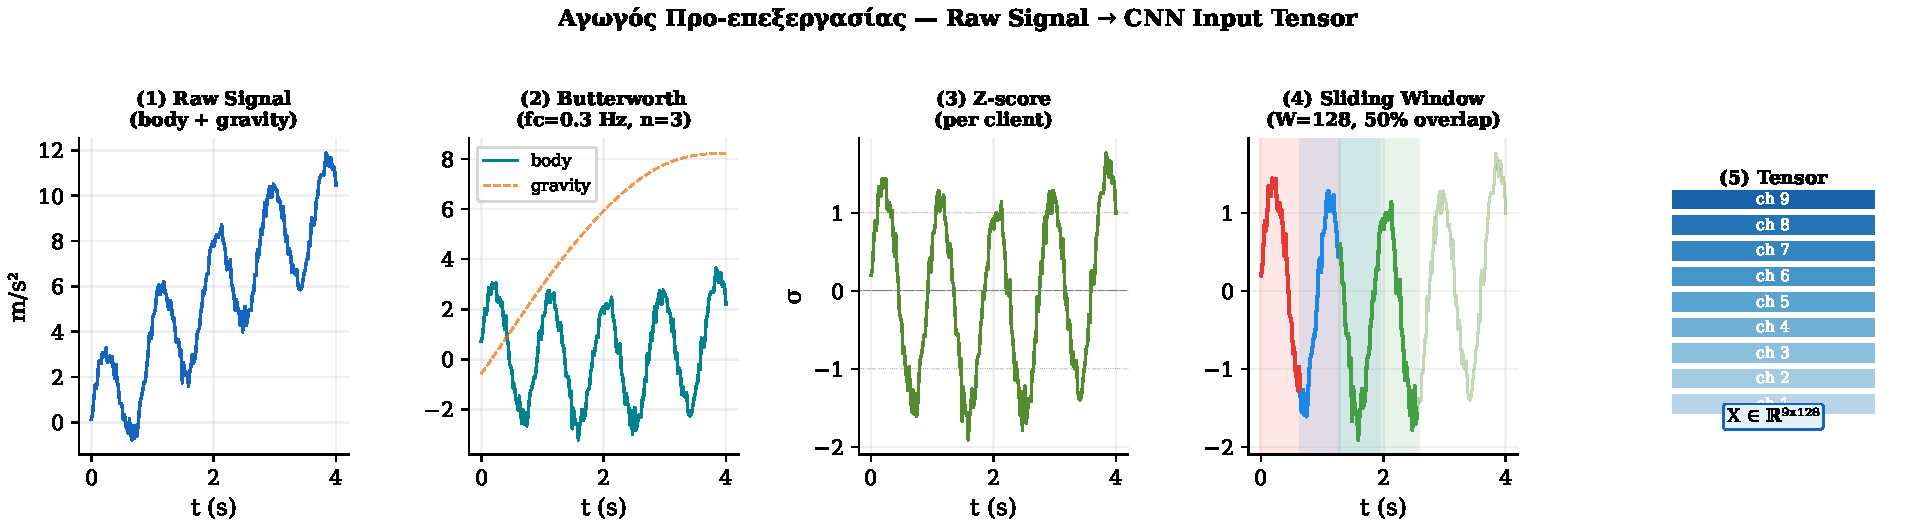
\includegraphics[width=\textwidth]{eda_preprocessing_pipeline.pdf}
    \caption{Αγωγός προ-επεξεργασίας από ακατέργαστο σήμα αισθητήρα
    σε τανυστή εισόδου CNN. (1)~Ακατέργαστο σήμα (κίνηση + βαρύτητα).
    (2)~Φίλτρο Butterworth 3ης τάξης ($f_c = 0{,}3$\,Hz): εξαγωγή
    βαρύτητας (πορτοκαλί) και σώματος (κυανό).
    (3)~Z-score κανονικοποίηση ανά client.
    (4)~Sliding window ($W=128$, 50\% επικάλυψη).
    (5)~Τανυστής εξόδου $\mathbf{X} \in \mathbb{R}^{9 \times 128}$.
    Ο αγωγός εφαρμόζεται τοπικά σε κάθε FL client.}
    \label{fig:preprocessing_pipeline}
\end{figure}

Ο αγωγός εφαρμόζεται \textbf{τοπικά σε κάθε client}, σύμφωνα
με τις αρχές του FL: τα στατιστικά κανονικοποίησης ($\mu_c$,
$\sigma_c$) δεν κοινοποιούνται στον server, διατηρώντας την
ιδιωτικότητα των δεδομένων. Η έξοδος κάθε client είναι ένα
τοπικό σύνολο παραθύρων $\{\mathbf{X}^{(k)}, y^{(k)}\}_{k=1}^{K_i}$,
όπου $K_i$ ο αριθμός παραθύρων του client $i$.

Αξίζει να σημειωθεί ότι ο αγωγός αυτός δεν εφαρμόζει μείωση διαστατικότητας (dimensionality reduction) ή επιλογή χαρακτηριστικών (feature selection) — τεχνικές που έχουν εξεταστεί εκτενώς στη βιβλιογραφία~\cite{Zebari2022}. Η επιλογή αυτή γίνεται σκόπιμα: ο 1D-CNN εκτελεί αυτόματη εξαγωγή ιεραρχικών χαρακτηριστικών από το ακατέργαστο σήμα, χωρίς να απαιτείται προηγούμενη χειροκίνητη επιλογή. Η χρήση του συνόλου των 9 καναλιών (3 επιταχύνσεις, 3 γωνιακές ταχύτητες, 3 body accelerations) χωρίς περαιτέρω μείωση επιτρέπει στο δίκτυο να ανακαλύψει από μόνο του ποιοι συνδυασμοί καναλιών είναι πληροφοριακοί για κάθε κλάση δραστηριότητας — προσέγγιση που αποδείχθηκε ανώτερη των hand-crafted features στα πειράματα αξιολόγησης~\cite{Chen2021, Hammerla2016}.


% ── Κεφάλαιο 4: Υλοποίηση & Μεθοδολογία ────────────────────

\chapter{Υλοποίηση και Μεθοδολογία}
\label{ch:implementation}

Το κεφάλαιο αυτό παρουσιάζει αναλυτικά την τεχνική υλοποίηση του συστήματος σε τρεις ενότητες: τη σχεδίαση του 1D-CNN μοντέλου HAR, το Federated Learning πλαίσιο server-client με FedAvg, και τον μηχανισμό κινήτρων Stackelberg. Κάθε ενότητα συνδέει την αρχιτεκτονική επιλογή με τη θεωρητική τεκμηρίωση του Κεφαλαίου~\ref{ch:background}.

% ── §4.1: Σχεδιασμός του Νευρωνικού Δικτύου ─────────────────

\section{Σχεδιασμός του Νευρωνικού Δικτύου}
\label{sec:cnn_design}

Η βαθιά εκμάθηση παρέχει τα κατάλληλα εργαλεία για αυτόματη εξαγωγή χαρακτηριστικών από σύνθετα δεδομένα χωρίς χειροκίνητη μηχανική χαρακτηριστικών \cite{Goodfellow2016}. Για τον σκοπό αυτόν σχεδιάστηκε ένα μονοδιάστατο συνελικτικό νευρωνικό δίκτυο (1D-CNN) κατάλληλο για ταξινόμηση δραστηριότητας σε περιβάλλον Federated Learning.

\subsection{Μορφή Εισόδου}

Το σύστημα χρησιμοποιεί τα προ-εξαχθέντα features του dataset AAL, τα οποία αποτελούνται από 561 στατιστικά χαρακτηριστικά χρονικού και συχνοτικού πεδίου ανά παράθυρο~\cite{AAL_UCI2016}. Κάθε δείγμα εισόδου έχει μορφή τανυστή $\mathbf{x} \in \mathbb{R}^{1 \times 561}$, όπου το ένα κανάλι αντιπροσωπεύει την πλήρη ακολουθία feature. Τα 561 features αντιμετωπίζονται ως μονοδιάστατη ακολουθία, επιτρέποντας στις Conv1d λειτουργίες να εντοπίσουν τοπικές συσχετίσεις μεταξύ γειτονικών χαρακτηριστικών.

\subsection{Αρχιτεκτονική}

Το δίκτυο αποτελείται από δύο συνελικτικά blocks ακολουθούμενα από πλήρως συνδεδεμένο κεφαλή ταξινόμησης, όπως απεικονίζεται στο Σχήμα~\ref{fig:cnn_arch} και αναλύεται στον Πίνακα~\ref{tab:cnn_arch}:

\begin{figure}[H]
\centering
\begin{tikzpicture}[
  node distance=0.55cm,
  box/.style={rectangle, draw=black!70, rounded corners=3pt,
              minimum width=2.2cm, minimum height=0.65cm,
              font=\scriptsize, align=center, fill=#1},
  arr/.style={-{Stealth[length=4pt]}, thick, gray!70},
  lbl/.style={font=\tiny, text=gray!80}
]

% Nodes (top to bottom)
\node[box=blue!12]   (inp)  {Είσοδος\\$[B,1,561]$};
\node[box=orange!20, below=of inp]  (c1)   {Conv1d(64)\\$k{=}9$, pad=4};
\node[box=yellow!30, below=of c1]   (bn1)  {BatchNorm1d(64)\\ReLU};
\node[box=green!15,  below=of bn1]  (mp1)  {MaxPool1d(2)\\$[B,64,280]$};
\node[box=orange!20, below=of mp1]  (c2)   {Conv1d(128)\\$k{=}9$, pad=4};
\node[box=yellow!30, below=of c2]   (bn2)  {BatchNorm1d(128)\\ReLU};
\node[box=green!15,  below=of bn2]  (mp2)  {MaxPool1d(2)\\$[B,128,140]$};
\node[box=gray!15,   below=of mp2]  (flat) {Flatten\\$[B,17920]$};
\node[box=purple!15, below=of flat] (drop) {Dropout(0.5)\\Linear(17920→128)};
\node[box=red!15,    below=of drop] (out)  {Linear(128→6)\\Softmax};

% Arrows
\foreach \s/\t in {inp/c1, c1/bn1, bn1/mp1, mp1/c2, c2/bn2, bn2/mp2, mp2/flat, flat/drop, drop/out}
  \draw[arr] (\s) -- (\t);

% Brace labels for blocks
\draw[decorate, decoration={brace,amplitude=5pt}, thick, gray!60]
  ([xshift=1.2cm]c1.north east) -- ([xshift=1.2cm]mp1.south east)
  node[midway, right=6pt, lbl] {Block 1};
\draw[decorate, decoration={brace,amplitude=5pt}, thick, gray!60]
  ([xshift=1.2cm]c2.north east) -- ([xshift=1.2cm]mp2.south east)
  node[midway, right=6pt, lbl] {Block 2};

\end{tikzpicture}
\caption{Αρχιτεκτονική 1D-CNN για HAR: δύο συνελικτικά blocks (Conv1d → BN → ReLU → MaxPool) ακολουθούμενα από πλήρως συνδεδεμένη κεφαλή ταξινόμησης.}
\label{fig:cnn_arch}
\end{figure}

Το δίκτυο αποτελείται από δύο συνελικτικά blocks ακολουθούμενα από πλήρως συνδεδεμένο κεφαλή ταξινόμησης (Πίνακας~\ref{tab:cnn_arch}):

\begin{table}[h]
\centering
\caption{Αρχιτεκτονική HAR-CNN: διαστάσεις τανυστή ανά επίπεδο.}
\label{tab:cnn_arch}
\begin{tabular}{llcc}
\hline
\textbf{Επίπεδο} & \textbf{Τύπος} & \textbf{Παράμετροι} & \textbf{Έξοδος} \\
\hline
Είσοδος & — & — & $[B, 1, 561]$ \\
Conv1d + BN + ReLU & συνελικτικό & $1{\to}64$, $k{=}9$ & $[B, 64, 561]$ \\
MaxPool1d(2) & υποδειγματοληψία & — & $[B, 64, 280]$ \\
Conv1d + BN + ReLU & συνελικτικό & $64{\to}128$, $k{=}9$ & $[B, 128, 280]$ \\
MaxPool1d(2) & υποδειγματοληψία & — & $[B, 128, 140]$ \\
Flatten & αναδιαμόρφωση & — & $[B, 17920]$ \\
Dropout(0.5) + Linear & πλήρης σύνδεση & $17920{\to}128$ & $[B, 128]$ \\
Linear & έξοδος & $128{\to}6$ & $[B, 6]$ \\
\hline
\end{tabular}
\end{table}

Κάθε συνελικτικό block ακολουθεί τη δομή:

\begin{equation}
\mathbf{h} = \text{MaxPool}\bigl(\text{ReLU}\bigl(\text{BN}\bigl(\text{Conv1d}(\mathbf{x})\bigr)\bigr)\bigr)
\label{eq:conv_block}
\end{equation}

όπου $\text{BN}$ συμβολίζει το Batch Normalization \cite{He2016}. Η κανονικοποίηση batch είναι ιδιαίτερα κρίσιμη σε περιβάλλον FL, καθώς κάθε client έχει ιδιάζουσα κατανομή δεδομένων — το BN σταθεροποιεί τη ροή gradients ανεξάρτητα από τα per-client statistics.

\subsection{Κεφαλή Ταξινόμησης}

Μετά τη δισδιάστατη αναδιαμόρφωση (flatten), η αλληλουχία $[B, 128 \times 140] = [B, 17920]$ οδηγείται σε δύο πλήρως συνδεδεμένα επίπεδα με ενδιάμεσο Dropout($p{=}0.5$). Το Dropout λειτουργεί ως κανονιστής — αποτρέπει την υπερπροσαρμογή (overfitting) σε μικρά client datasets, που είναι συνηθισμένη κατάσταση στο FL \cite{Goodfellow2016}.

Η έξοδος είναι ένα διάνυσμα logits $\hat{\mathbf{y}} \in \mathbb{R}^6$. Κατά την εκπαίδευση, το CrossEntropyLoss υπολογίζει απευθείας απο τα logits χωρίς επιπλέον softmax, για αριθμητική σταθερότητα.

\subsection{Εκπαίδευση}

Ως βελτιστοποιητής χρησιμοποιείται ο Adam \cite{Kingma2015} με $\text{lr} = 10^{-3}$, ο οποίος προσαρμόζει αυτόματα το βήμα μάθησης ανά παράμετρο και συγκλίνει αξιόπιστα χωρίς ευαίσθητη ρύθμιση. Συνολικά, το δίκτυο έχει \textbf{2.369.542 εκπαιδεύσιμες παραμέτρους}. Πλήρης κώδικας της κλάσης \texttt{HAR\_CNN} είναι διαθέσιμος στο αποθετήριο κώδικα της εργασίας.
% ── §4.2: Ανάπτυξη του Federated Framework ───────────────────

\section{Ανάπτυξη του Federated Framework}
\label{sec:fl_framework}

Το Federated Learning επιτρέπει σε πολλούς συμμετέχοντες να εκπαιδεύσουν κοινό μοντέλο χωρίς να κοινοποιήσουν τα raw δεδομένα τους~\cite{McMahan2017}. Στο πλαίσιο αυτής της διπλωματικής, κάθε client αντιστοιχεί σε έναν χρήστη του dataset AAL με τα δικά του δεδομένα δραστηριότητας. Το σύστημα περιλαμβάνει 22 clients — έναν ανά subject του training set. Η υλοποίηση βασίστηκε στον κώδικα αναφοράς του N.\ Pavlidis~\cite{PavlidisFL2021}, που παρέχει ένα καλά δοκιμασμένο template FL συστήματος με PyTorch, διασφαλίζοντας ορθή αρχιτεκτονική server-client από την αρχή και αποφεύγοντας κοινά pitfalls στην υλοποίηση κατανεμημένης εκπαίδευσης.

\subsection{Αρχιτεκτονική Server-Client}

Ο server λειτουργεί ως συντονιστής: αρχικοποιεί το global μοντέλο, επιλέγει clients ανά γύρο, συλλέγει τοπικά ενημερωμένα weights και εκτελεί aggregation. Ο client λαμβάνει τα global parameters, εκπαιδεύει τοπικά, και αποστέλλει τα ενημερωμένα weights — ποτέ τα raw δεδομένα.

Η επικοινωνία ανά γύρο $t$ ακολουθεί τα παρακάτω βήματα:

\begin{enumerate}
    \item \textbf{Επιλογή clients:} Ο server επιλέγει υποσύνολο $S_t \subseteq \mathcal{N}$ με $|S_t| = K$.
    \item \textbf{Αποστολή global model:} Κάθε client $i \in S_t$ λαμβάνει τα global parameters $\boldsymbol{\theta}^{(t)}$.
    \item \textbf{Τοπική εκπαίδευση:} Κάθε client εκπαιδεύει για $E$ εποχές:
    $\boldsymbol{\theta}_i^{(t+1)} \gets \text{LocalTrain}(\boldsymbol{\theta}^{(t)}, \mathcal{D}_i)$.
    \item \textbf{Αποστολή ενημερωμένων weights:} Κάθε client στέλνει $\boldsymbol{\theta}_i^{(t+1)}$ και $n_i$ στον server.
    \item \textbf{FedAvg aggregation:} Ο server υπολογίζει το νέο global model:
\end{enumerate}

\begin{equation}
\boldsymbol{\theta}^{(t+1)} = \sum_{i \in S_t} \frac{n_i}{N_t} \cdot \boldsymbol{\theta}_i^{(t+1)}
\tag{\ref{eq:fedavg}}
\end{equation}

όπου $n_i = |\mathcal{D}_i|$ ο αριθμός δειγμάτων client $i$ και $N_t = \sum_{i \in S_t} n_i$.

\subsection{Τοπική Εκπαίδευση}

Κάθε client εκτελεί $E = 5$ τοπικές εποχές με βελτιστοποιητή Adam ($\text{lr} = 10^{-3}$) και συνάρτηση απώλειας CrossEntropyLoss. Η επιλογή $E = 5$ αποτελεί ισορροπία μεταξύ δύο αντικρουόμενων στόχων: \textit{(α)} αρκετές εποχές ώστε η τοπική εκπαίδευση να είναι αποτελεσματική, και \textit{(β)} λίγες εποχές ώστε να αποφεύγεται το φαινόμενο client drift~\cite{Li2020}, όπου τα τοπικά μοντέλα αποκλίνουν υπερβολικά από το global.

\subsection{Στάθμιση FedAvg}

Η στάθμιση $n_i / N_t$ εξασφαλίζει ότι clients με περισσότερα δεδομένα συνεισφέρουν αναλογικά περισσότερο στο global μοντέλο. Στο συγκεκριμένο σενάριο, οι 22 clients έχουν $n_i \in [130, 280]$ δείγματα (μέσο: $\approx 193$), οπότε η Non-IID επίδραση της ανισομερούς κατανομής είναι μέτρια.

\subsection{Γύροι Επικοινωνίας}

Το σύστημα εκτελεί $T = 20$ γύρους FL. Σε κάθε γύρο συμμετέχουν όλοι οι 22 clients (\texttt{FRACTION\_FIT = 1.0}). Η σύγκλιση του αλγορίθμου αποτιμάται πειραματικά σε επόμενο στάδιο της εργασίας.

\subsection{Non-IID Διαχωρισμός}

Ο φυσικός διαχωρισμός των δεδομένων ανά subject (\texttt{by\_subject}) αποτελεί το πιο ρεαλιστικό σενάριο FL: κάθε smartphone ανήκει σε έναν χρήστη και περιέχει μόνο τα δικά του δεδομένα~\cite{Yang2019}. Αυτό δημιουργεί ετερογένεια κατανομής (Non-IID), η οποία έχει αναλυθεί ποσοτικά στην ενότητα~\ref{sec:eda} μέσω της μέτρησης JSD² (μέσο: 0.040).

% ── §4.3: Ο Μηχανισμός Κινήτρων ─────────────────────────────

\section{Ο Μηχανισμός Κινήτρων}
\label{sec:incentive_mechanism}

Στην παρούσα ενότητα παρουσιάζεται διεξοδικά ο σχεδιασμός του μηχανισμού κινήτρων που είναι κεντρική
ερευνητική συνεισφορά της εργασίας. Αρχικά αναλύεται γιατί ένα FL σύστημα δεν λειτουργεί χωρίς τέτοιο
μηχανισμό (§\ref{subsec:inc_problem}), στη συνέχεια αποσυντίθεται ο χώρος σχεδιασμού σε τρεις ανεξάρτητες
συνιστώσες (§\ref{subsec:inc_taxonomy}), παρουσιάζονται \textbf{επτά υποψήφιοι μηχανισμοί} με
αυξανόμενη πολυπλοκότητα (§\ref{subsec:inc_candidates}), τίθενται κριτήρια αξιολόγησης
(§\ref{subsec:inc_criteria}), διεξάγεται συγκριτική ανάλυση (§\ref{subsec:inc_comparison}) και
καταλήγουμε σε \textbf{shortlist τριών μηχανισμών} (§\ref{subsec:inc_shortlist}) και στον
προτεινόμενο υβριδικό μηχανισμό που αξιολογείται πειραματικά στη συνέχεια.

% =============================================================
\subsection{Το Πρόβλημα και οι Σχεδιαστικοί Στόχοι}
\label{subsec:inc_problem}

Στο FedAvg~\cite{McMahan2017} κάθε client $i$ ασκεί \emph{προσπάθεια} (effort) $e_i \in [0,1]$ που
αντιστοιχεί στο ποσοστό των τοπικών επαναλήψεων που πραγματικά εκτελούνται και στην ποιότητα των
gradients που αποστέλλει στον server. Η προσπάθεια συνεπάγεται \emph{κόστος} $c_i(e_i)$ — μπαταρία,
CPU, χρόνος — που επωμίζεται μόνος του ο χρήστης. Χωρίς αντιστάθμισμα, η \textbf{κυρίαρχη στρατηγική}
(\emph{dominant strategy}) κάθε ορθολογικού client είναι $e_i^* = 0$: συμμετέχει συνωμοτικά αλλά δεν
συνεισφέρει — το γνωστό \textbf{free-rider problem}~\cite{Kang2019, Yu2020}.

Επιπλέον, στο πραγματικό σενάριο AAL οι χρήστες δεν έχουν \emph{ομοιογενή} ποιότητα δεδομένων: όπως
αποδείχθηκε ποσοτικά στο §\ref{sec:eda} (JSD$^2$ μέσος $0{,}040$, $31{,}8\%$ subjects $> 0{,}05$),
ορισμένοι έχουν δεδομένα κρίσιμα για τη γενίκευση ενώ άλλοι όχι. Ένας μηχανισμός που τους ανταμείβει
\emph{ομοιόμορφα} είναι ταυτόχρονα άδικος (αδικεί τους ποιοτικούς συνεισφέροντες) και
\emph{αναποτελεσματικός} (δεν δημιουργεί κίνητρο για διαφοροποίηση).

\paragraph{Σχεδιαστικοί στόχοι.} Ένας μηχανισμός κινήτρων για το παρόν σύστημα οφείλει ταυτόχρονα να
ικανοποιεί:

\begin{enumerate}
    \item \textbf{Ορθολογικότητα συμμετοχής (Individual Rationality, IR):} κάθε client πρέπει να έχει
    μη-αρνητική αναμενόμενη χρησιμότητα όταν συμμετέχει. Διαφορετικά αποχωρεί.
    \item \textbf{Συμβατότητα κινήτρων (Incentive Compatibility, IC):} αν ο μηχανισμός απαιτεί ο
    client να αναφέρει ιδιωτική πληροφορία (π.χ. το κόστος του), η ειλικρινής αναφορά πρέπει να είναι
    βέλτιστη.
    \item \textbf{Δικαιοσύνη (Fairness):} η αμοιβή να είναι ανάλογη της \emph{αξίας συνεισφοράς}, όχι
    μόνο του όγκου δεδομένων.
    \item \textbf{Υπολογιστική εφικτότητα:} ο μηχανισμός πρέπει να εκτελείται σε λογικό χρόνο για
    $N = 22$ clients σε CPU.
    \item \textbf{Ανθεκτικότητα (Robustness):} σε στατιστικό θόρυβο, σε κακόβουλους clients, και σε
    cold-start περιπτώσεις.
    \item \textbf{Συμβατότητα με ιδιωτικότητα:} ο server δεν πρέπει να χρειάζεται πρόσβαση σε raw data.
\end{enumerate}

Όπως θα φανεί, καμία μεμονωμένη επιλογή δεν ικανοποιεί όλους αυτούς τους στόχους ταυτόχρονα — και
ακριβώς γι' αυτό εξετάζονται πολλαπλοί υποψήφιοι.

% =============================================================
\subsection{Δομικά Στοιχεία ενός Μηχανισμού}
\label{subsec:inc_taxonomy}

Ένας μηχανισμός κινήτρων FL αποσυντίθεται φυσικά σε \textbf{τρεις ορθογώνιες συνιστώσες} που μπορούν
να συνδυαστούν ανεξάρτητα:

\begin{enumerate}[label=(\Alph*)]
    \item \textbf{Μέτρηση συνεισφοράς} ($\hat{\varphi}_i$): πώς ποσοτικοποιείται η αξία κάθε client.
    Επιλογές: όγκος δεδομένων, LOO, Shapley, gradient similarity, influence functions, reputation
    history.

    \item \textbf{Κατανομή αμοιβών} ($r_i$): πώς μετατρέπεται η μέτρηση σε χρηματική / υπολογιστική
    αμοιβή. Επιλογές: αναλογική, top-$K$ selection, auction-based payment, threshold-based,
    Shapley payment, contract menu.

    \item \textbf{Στρατηγικό πλαίσιο αλληλεπίδρασης}: πώς διαμορφώνεται η ισορροπία μεταξύ server και
    clients. Επιλογές: χωρίς strategic interaction (descriptive), Stackelberg single-round, repeated
    Stackerberg, reverse auction (VCG), contract theory, mean-field game.
\end{enumerate}

Στον Πίνακα~\ref{tab:inc_components} συνοψίζονται οι επιμέρους επιλογές κάθε συνιστώσας. Κάθε
\emph{ολοκληρωμένος μηχανισμός} είναι ένας συγκεκριμένος τριάδας~(A,~B,~C). Οι 7 υποψήφιοι που
αναλύονται παρακάτω είναι αντιπροσωπευτικά μονοπάτια αυτού του χώρου.

\begin{table}[H]
    \centering
    \caption{Χώρος σχεδιασμού: επιλογές ανά συνιστώσα μηχανισμού κινήτρων.}
    \label{tab:inc_components}
    \footnotesize
    \begin{tabular}{p{0.27\textwidth} p{0.32\textwidth} p{0.32\textwidth}}
        \toprule
        \textbf{(A) Μέτρηση συνεισφοράς} & \textbf{(B) Κατανομή αμοιβών} & \textbf{(C) Στρατηγικό πλαίσιο} \\
        \midrule
        Όγκος δεδομένων ($n_i$) & Αναλογική ($\varphi_i / \sum_j \varphi_j$) & Καμία αλληλεπίδραση \\
        LOO ($v(\mathcal N) - v(\mathcal N \setminus i)$) & Top-$K$ selection & Stackelberg single-round \\
        Shapley value (exact / MC) & Threshold (κατώφλι ποιότητας) & Repeated Stackelberg \\
        Gradient cosine similarity & Auction payment (VCG) & Reverse auction \\
        Influence functions & Shapley payment (efficient) & Contract theory \\
        Reputation (multi-round) & Contract menu & Mean-field game \\
        \bottomrule
    \end{tabular}
\end{table}

% =============================================================
\subsection{Επτά Υποψήφιοι Μηχανισμοί}
\label{subsec:inc_candidates}

Ακολουθεί η αναλυτική περιγραφή επτά μηχανισμών (\textbf{M1}--\textbf{M7}), κατά αυξάνουσα
πολυπλοκότητα και θεωρητική φιλοδοξία. Για κάθε έναν δίνονται: (i) η μαθηματική διατύπωση, (ii) ο
αλγόριθμος υπολογισμού, (iii) τα πλεονεκτήματα/μειονεκτήματα και (iv) η υπολογιστική πολυπλοκότητα.

% ─────────────────────────────────────────────────────────────
\subsubsection{M1 — Όγκο-Αναλογικός Μηχανισμός (Volume-Proportional)}
\label{subsubsec:M1_volume}

\textbf{Συνιστώσες:} (A) volume contribution, (B) proportional allocation, (C) καμία στρατηγική αλληλεπίδραση.

\textbf{Διατύπωση.} Η συνεισφορά κάθε client μετράται με τον αριθμό δειγμάτων του:
\begin{equation}
    \hat{\varphi}_i^{\,(\text{vol})} = \frac{n_i}{\sum_{j=1}^{N} n_j}
    \label{eq:M1_contrib}
\end{equation}
και η αμοιβή κατανέμεται αναλογικά: $r_i = \hat{\varphi}_i^{\,(\text{vol})} \cdot R$.

\textbf{Πλεονεκτήματα.} Υπολογιστικό κόστος $\mathcal{O}(1)$· δεν απαιτείται καμία επιπλέον FL
αξιολόγηση. Συμβατό με το κλασικό FedAvg~\cite{McMahan2017} γιατί χρησιμοποιεί ήδη τα ίδια βάρη.
Διαφανές και άμεσα κατανοητό από τους χρήστες.

\textbf{Μειονεκτήματα.} \emph{Αγνοεί την ποιότητα} δεδομένων: ένας client με 1000 σχεδόν ίδια
παράθυρα WALKING αμείβεται το ίδιο με έναν με 1000 ποικίλα και ισορροπημένα. Επίσης, \emph{δεν
αντιμετωπίζει το free-rider} — ένας client μπορεί να στείλει αλλοιωμένα gradients και να αμείβεται.

\textbf{Πολυπλοκότητα.} $\mathcal{O}(1)$ για όλους τους $N$ clients (μόνο μια άθροιση). Καμία FL
αξιολόγηση.

\textbf{Ρόλος στην εργασία.} Χρησιμοποιείται ως \textbf{baseline} για να εκτιμηθεί πόση επιπλέον
δικαιοσύνη / απόδοση φέρνουν οι πιο πολύπλοκοι μηχανισμοί.

% ─────────────────────────────────────────────────────────────
\subsubsection{M2 — LOO + Αναλογική Κατανομή + Stackelberg}
\label{subsubsec:M2_loo_stackelberg}

\textbf{Συνιστώσες:} (A) LOO contribution, (B) proportional allocation, (C) Stackelberg single-round.

\textbf{Διατύπωση.} Η συνεισφορά εκτιμάται με Leave-One-Out:
\begin{equation}
    \hat{\varphi}_i^{\,(\text{LOO})} = \max\big(0,\, v(\mathcal{N}) - v(\mathcal{N} \setminus \{i\})\big)
    \label{eq:M2_loo}
\end{equation}
όπου $v(S)$ η accuracy του global μοντέλου μετά από $E_{\text{LOO}} = 3$ FL γύρους με τους clients
του $S$. Η αποκοπή στο μηδέν αποκλείει αρνητικές contributions (πιθανώς adversarial).

Η αμοιβή κατανέμεται αναλογικά:
\begin{equation}
    r_i = \max\!\left(r_{\min},\; \frac{\hat{\varphi}_i^{\,(\text{LOO})}}{\sum_{j} \hat{\varphi}_j^{\,(\text{LOO})}} \cdot R\right)
    \label{eq:M2_reward}
\end{equation}
με $r_{\min} = 0{,}01$ (ελάχιστη συμμετοχή). Τέλος, κάθε client επιλύει το πρόβλημα Stackelberg
\begin{equation}
    \max_{e_i \in [0,1]} \; u_i(e_i) = r_i \cdot e_i - c \cdot e_i^2
    \implies e_i^* = \frac{r_i}{2c}
    \label{eq:M2_effort}
\end{equation}
με $c = 0{,}5$. Η ισορροπία είναι μοναδική λόγω της κυρτότητας του κόστους~\cite{Sarikaya2020}.

\textbf{Πλεονεκτήματα.} Πιστή ποσοτικοποίηση \emph{οριακής} συνεισφοράς — απαντά άμεσα στην ερώτηση
"πόσο χάνω αν χάσω αυτόν τον client;". Closed-form λύση Stackerberg → άμεση ερμηνευσιμότητα. Το
$r_{\min}$ διασφαλίζει IR.

\textbf{Μειονεκτήματα.} (i) Μη-αρθροιστική: $\sum_i \hat{\varphi}_i^{\,(\text{LOO})} \neq v(\mathcal N)$,
οπότε το αξίωμα efficiency του Shapley παραβιάζεται. (ii) Αγνοεί διαδραστικά effects (clients
συμπληρωματικοί δεν αναγνωρίζονται). (iii) Single-round: ευάλωτο σε στοχαστικό θόρυβο μιας μεμονωμένης
LOO αξιολόγησης.

\textbf{Πολυπλοκότητα.} $\mathcal{O}(N+1)$ FL αξιολογήσεις, καθεμία $\mathcal{O}(E_{\text{LOO}} \cdot N
\cdot E_{\text{local}})$. Για $N=22$, $E_{\text{LOO}}=3$, $E_{\text{local}}=5$: περίπου 7\,200 τοπικές
περάσεις, $\sim$3 λεπτά σε CPU.

% ─────────────────────────────────────────────────────────────
\subsubsection{M3 — Monte Carlo Shapley + Αναλογική + Stackelberg}
\label{subsubsec:M3_shapley_stackelberg}

\textbf{Συνιστώσες:} (A) MC Shapley, (B) proportional allocation, (C) Stackelberg.

\textbf{Διατύπωση.} Η ακριβής Shapley value~\cite{Shapley1953} ορίζεται ως
\begin{equation}
    \varphi_i = \sum_{S \subseteq \mathcal N \setminus \{i\}}
                \frac{|S|!\,(N-|S|-1)!}{N!} \big[v(S \cup \{i\}) - v(S)\big]
    \label{eq:shapley_exact}
\end{equation}
και ικανοποιεί τα τέσσερα αξιώματα δικαιοσύνης (efficiency, symmetry, null player, linearity). Ωστόσο
απαιτεί $2^N$ αξιολογήσεις — απαγορευτικό για $N=22$ ($\approx 4{,}2 \cdot 10^6$ υποσύνολα).

Η \emph{Monte Carlo} προσέγγιση~\cite{Jia2020} δειγματοληπτεί $M$ τυχαίες μεταθέσεις και υπολογίζει
οριακές συνεισφορές:
\begin{equation}
    \tilde{\varphi}_i = \frac{1}{M} \sum_{m=1}^{M} \big[v(S_i^{(m)} \cup \{i\}) - v(S_i^{(m)})\big]
    \label{eq:M3_mcshapley}
\end{equation}
όπου $S_i^{(m)}$ είναι το σύνολο clients πριν τον $i$ στη μετάθεση $m$. Η σύγκλιση είναι
$\mathcal{O}(\sigma / \sqrt{M})$. Στη βιβλιογραφία χρησιμοποιούνται τιμές $M$ της τάξης δεκάδων για σταθερή κατάταξη.

Η κατανομή αμοιβών και η Stackelberg ισορροπία είναι ίδιες με τον M2 (εξισώσεις~\ref{eq:M2_reward},
\ref{eq:M2_effort}).

\textbf{Πλεονεκτήματα.} \emph{Θεωρητικά βέλτιστος} — ο Shapley είναι ο μοναδικός τύπος που ικανοποιεί
τα τέσσερα αξιώματα δικαιοσύνης ταυτόχρονα (Shapley 1953). Πιάνει διαδραστικά effects: clients που
είναι χρήσιμοι μόνο σε συνδυασμό αξιολογούνται σωστά.

\textbf{Μειονεκτήματα.} \emph{Υπολογιστικά ακριβός}: $\mathcal{O}(M \cdot N)$ FL αξιολογήσεις. Για
$M=50$, $N=22$: $\sim$2 ώρες σε CPU. Επιπλέον, η εκτίμηση έχει στατιστική variance — επανεκτέλεση με
διαφορετικό seed δίνει ελαφρώς διαφορετικές τιμές.

\textbf{Πολυπλοκότητα.} $\mathcal{O}(M \cdot N)$ FL αξιολογήσεις. Στην πράξη, $\sim$120 λεπτά runtime.

% ─────────────────────────────────────────────────────────────
\subsubsection{M4 — Gradient Cosine Similarity (Online)}
\label{subsubsec:M4_gradient}

\textbf{Συνιστώσες:} (A) gradient cosine similarity, (B) προσαρμοσμένη γραμμική κατανομή, (C) χωρίς
ρητή στρατηγική αλληλεπίδραση (descriptive).

\textbf{Διατύπωση.} Η συνεισφορά κάθε client σε έναν γύρο $t$ εκτιμάται από την ευθυγράμμιση του
τοπικού του gradient με το global update~\cite{Xu2021}:
\begin{equation}
    \hat{\varphi}_i^{\,(\text{grad})}(t) =
    \frac{1}{2}\Big(1 + \frac{\Delta\theta_i^{(t)} \cdot \Delta\theta_{\text{global}}^{(t)}}
                                  {\|\Delta\theta_i^{(t)}\| \, \|\Delta\theta_{\text{global}}^{(t)}\|}\Big)
    \label{eq:M4_cossim}
\end{equation}
όπου $\Delta\theta_i^{(t)} = \theta_i^{(t)} - \theta_{\text{global}}^{(t-1)}$ το τοπικό update και
$\Delta\theta_{\text{global}}^{(t)}$ το συνδυασμένο global update. Η κανονικοποίηση στο διάστημα
$[0,1]$ διευκολύνει την κατανομή.

Η αμοιβή ανά γύρο: $r_i^{(t)} = \hat{\varphi}_i^{\,(\text{grad})}(t) \cdot R / N_{\text{active}}$,
όπου $N_{\text{active}}$ οι ενεργοί clients του γύρου.

\textbf{Πλεονεκτήματα.} \emph{Online}: η εκτίμηση γίνεται \emph{ταυτόχρονα} με την εκπαίδευση, χωρίς
επιπλέον FL γύρους. \emph{Pay-per-round}: μπορεί να αμείβει σε κάθε γύρο, ευνοώντας συνεχή συμμετοχή.
Πιάνει \emph{την κατεύθυνση} και όχι μόνο το μέγεθος της συνεισφοράς — ένας client που "τραβάει" το
μοντέλο σε αντίθετη κατεύθυνση εντοπίζεται άμεσα.

\textbf{Μειονεκτήματα.} (i) Θορυβώδης σε μεμονωμένο γύρο — απαιτεί smoothing μεταξύ γύρων (π.χ.
exponential moving average). (ii) Δεν διαφορίζει μεταξύ "θορύβου" και \emph{niche} χρήσιμης
πληροφορίας: ένας client με σπάνιες αλλά νόμιμες κατηγορίες μπορεί να έχει "κάθετη" κατεύθυνση και να
υπο-αμείβεται. (iii) Δεν έχει θεωρητικά αξιώματα δικαιοσύνης.

\textbf{Πολυπλοκότητα.} $\mathcal{O}(1)$ \emph{επιπλέον} ανά γύρο — μόνο pairwise dot products. Σχεδόν
δωρεάν.

% ─────────────────────────────────────────────────────────────
\subsubsection{M5 — Reputation-Based Multi-Round Mechanism}
\label{subsubsec:M5_reputation}

\textbf{Συνιστώσες:} (A) reputation history (συνδυασμός LOO + gradient similarity με exponential
smoothing), (B) reputation-weighted allocation με ρήτρα αποκλεισμού, (C) repeated game.

\textbf{Διατύπωση.} Η reputation κάθε client συσσωρεύεται με exponential smoothing:
\begin{equation}
    \rho_i^{(t)} = \beta \cdot \rho_i^{(t-1)} + (1-\beta) \cdot \tilde{\varphi}_i^{(t)}
    \label{eq:M5_reputation}
\end{equation}
με $\beta \in [0{,}8, 0{,}95]$ (μνήμη) και $\tilde{\varphi}_i^{(t)}$ μια στιγμιαία εκτίμηση
συνεισφοράς (π.χ. M4 ή light-LOO). Η αμοιβή κατανέμεται σε δύο επίπεδα:

\begin{itemize}
    \item Αν $\rho_i^{(t)} < \rho_{\text{thr}}$ (κατώφλι κακόβουλης συμπεριφοράς), ο client
    \emph{αποκλείεται} από τον επόμενο γύρο: $r_i^{(t+1)} = 0$.
    \item Αλλιώς: $r_i^{(t+1)} = \max(r_{\min},\, \rho_i^{(t)} / \sum_j \rho_j^{(t)} \cdot R)$.
\end{itemize}

\textbf{Πλεονεκτήματα.} \emph{Ανθεκτικός σε στιγμιαίο θόρυβο} — μια κακή εκτίμηση σε έναν γύρο δεν
καταστρέφει την αμοιβή. \emph{Φιλτράρει adversarial clients}: επανειλημμένα αρνητική συνεισφορά
οδηγεί σε αποκλεισμό. \emph{Δημιουργεί long-term κίνητρα} — ο client πρέπει να συμπεριφέρεται καλά
\emph{επί σειρά γύρων} για να συσσωρεύσει reputation.

\textbf{Μειονεκτήματα.} (i) \emph{Cold-start}: στους πρώτους γύρους όλοι έχουν ίδια reputation,
οπότε ο μηχανισμός εκφυλίζεται προς volume-based. (ii) Επιπλέον υπερπαράμετροι ($\beta$,
$\rho_{\text{thr}}$) που απαιτούν ρύθμιση. (iii) Ευπάθεια σε \emph{whitewashing} — κακόβουλος
client που "παίζει καλά" τους πρώτους γύρους και επιτίθεται μετά.

\textbf{Πολυπλοκότητα.} $\mathcal{O}(N)$ ανά γύρο για το EMA + όποια στιγμιαία εκτίμηση επιλεχθεί.
Συνολικά $\sim$10\,\% επιπλέον πάνω από το baseline.

% ─────────────────────────────────────────────────────────────
\subsubsection{M6 — Reverse Auction (VCG-Style)}
\label{subsubsec:M6_auction}

\textbf{Συνιστώσες:} (A) bid από τον client (ιδιωτικό cost type), (B) Vickrey-Clarke-Groves payment,
(C) reverse auction.

\textbf{Διατύπωση.} Κάθε client αναφέρει στον server το κόστος $b_i$ που απαιτεί για να εκτελέσει
$E_{\text{local}}$ γύρους εκπαίδευσης. Ο server επιλέγει υποσύνολο $\mathcal{S}^* \subseteq \mathcal N$
που μεγιστοποιεί την κοινωνική ωφέλεια:
\begin{equation}
    \mathcal{S}^* = \arg\max_{\mathcal{S} \subseteq \mathcal{N}}
                    \Big[v(\mathcal S) - \sum_{i \in \mathcal S} b_i\Big]
    \label{eq:M6_winners}
\end{equation}

Το VCG payment για κάθε νικητή $i \in \mathcal{S}^*$ είναι η \emph{εξωτερικότητα} (externality) που
επιβάλλει στους άλλους:
\begin{equation}
    r_i^{\text{VCG}} = \Big[v(\mathcal S^*_{-i}) - \sum_{j \in \mathcal S^*_{-i}} b_j\Big]
                    - \Big[v(\mathcal S^*) - \sum_{j \in \mathcal S^* \setminus \{i\}} b_j\Big]
    \label{eq:M6_vcg}
\end{equation}
όπου $\mathcal S^*_{-i}$ η βέλτιστη επιλογή \emph{αν δεν υπήρχε} ο client $i$.

\textbf{Πλεονεκτήματα.} \emph{Αποδεδειγμένα incentive-compatible} (αξίωμα Vickrey 1961, Clarke 1971,
Groves 1973): η ειλικρινής αναφορά $b_i = c_i$ είναι κυρίαρχη στρατηγική. \emph{Μεγιστοποιεί κοινωνική
ωφέλεια} (efficiency). Φυσικό fit όταν το \emph{cost type} κάθε χρήστη είναι ιδιωτικό και ετερογενές
(π.χ. κάποιοι έχουν παλαιότερα κινητά με μεγαλύτερο κόστος μπαταρίας).

\textbf{Μειονεκτήματα.} (i) \emph{Υπολογιστικά απαιτητικός}: το πρόβλημα επιλογής νικητών είναι
NP-hard στη γενική περίπτωση (απαιτεί $v(\mathcal S)$ για κάθε $\mathcal S \subseteq \mathcal N$). Στην
πράξη χρειάζεται greedy approximation με εγγυήσεις απόδοσης. (ii) \emph{Budget non-balanced}:
ο server μπορεί να πληρώσει περισσότερα από το συνολικό όφελος (έλλειμμα). (iii) Απαιτεί
\emph{collusion-resistance} — μηχανισμοί καρτέλ μπορούν να αλλοιώσουν την IC ιδιότητα.

\textbf{Πολυπλοκότητα.} $\mathcal{O}(2^N)$ για ακριβή λύση· $\mathcal{O}(N^2)$ με greedy
approximation και submodular value function. Για $N=22$: $\sim$8 λεπτά greedy, $\sim$30+ λεπτά
exact (απαγορευτικό).

% ─────────────────────────────────────────────────────────────
\subsubsection{M7 — Contract Theory με Ιδιωτικούς Cost Types}
\label{subsubsec:M7_contract}

\textbf{Συνιστώσες:} (A) προσπάθεια ως μη-παρατηρήσιμη (hidden action), (B) menu of contracts, (C)
mechanism design με adverse selection.

\textbf{Διατύπωση.} Σε αυτό το πλαίσιο~\cite{Zhan2023}, υποθέτουμε ότι κάθε client έχει \emph{ιδιωτικό
τύπο κόστους} $\theta_i$ που τραβιέται από κατανομή $F(\theta)$ γνωστή στον server. Το κόστος του
client είναι $c_i(e_i; \theta_i) = \theta_i \cdot e_i^2 / 2$ — clients υψηλού τύπου έχουν μεγαλύτερο
κόστος προσπάθειας.

Ο server προσφέρει \emph{menu από contracts} $\{(e_\theta, r_\theta)\}_{\theta \in \Theta}$, ένα ανά
δυνατό τύπο. Κάθε contract λέει "αν αναφέρεις τύπο $\theta$, εκτέλεσε προσπάθεια $e_\theta$ και πάρε
αμοιβή $r_\theta$". Με τους περιορισμούς IC και IR:
\begin{align}
    \text{IR:} \quad & r_\theta - c(e_\theta; \theta) \geq 0 \quad \forall \theta \\
    \text{IC:} \quad & r_\theta - c(e_\theta; \theta) \geq r_{\theta'} - c(e_{\theta'}; \theta) \quad \forall \theta, \theta'
\end{align}
ο server λύνει:
\begin{equation}
    \max_{\{(e_\theta, r_\theta)\}} \; \mathbb{E}_\theta\big[v(e_\theta) - r_\theta\big]
    \quad \text{υπό IR, IC}
    \label{eq:M7_contract}
\end{equation}

Σε διακριτό περιβάλλον τύπων (π.χ. high-cost / low-cost), η λύση δίνεται από κλασικά αποτελέσματα
mechanism design (Myerson 1981) και έχει closed form.

\textbf{Πλεονεκτήματα.} \emph{Θεωρητικά βέλτιστος} όταν υπάρχει heterogeneity κόστους και ιδιωτικότητα
τύπων — η περίπτωση του πραγματικού AAL (νεότεροι vs ηλικιωμένοι, νεότερα vs παλαιότερα κινητά).
Δίνει ταυτόχρονα IR + IC + κοινωνικά αποδοτική κατανομή. \emph{Αυτο-επιλεκτικό}: οι clients επιλέγουν
μόνοι τους το contract, αποκαλύπτοντας τον τύπο τους.

\textbf{Μειονεκτήματα.} (i) Απαιτεί \emph{γνώση της κατανομής} $F(\theta)$ — στην πράξη πρέπει να
εκτιμηθεί. (ii) Πιο πολύπλοκη υλοποίηση και debugging σε σχέση με Stackelberg. (iii) Δυσκολότερο να
γενικευτεί σε πιο σύνθετες δράσεις (πέραν της προσπάθειας).

\textbf{Πολυπλοκότητα.} $\mathcal{O}(|\Theta|^2)$ για διακριτούς τύπους (συνήθως $|\Theta| = 2$--$5$),
$\mathcal{O}(N \cdot |\Theta|)$ για evaluation σε όλους τους clients. Πρακτικά: $\sim$1--2 λεπτά.

% =============================================================
\subsection{Κριτήρια Αξιολόγησης}
\label{subsec:inc_criteria}

Για να συγκρίνουμε τους επτά μηχανισμούς, ορίζονται \textbf{πέντε κριτήρια} που αντιστοιχούν στους
σχεδιαστικούς στόχους της §\ref{subsec:inc_problem}:

\begin{enumerate}[label=\textbf{C\arabic*.}, leftmargin=2.5em]
    \item \textbf{Δικαιοσύνη (Fairness)}: ποσοτικοποιείται με τη συσχέτιση Pearson μεταξύ της αμοιβής
    $r_i$ και μιας \emph{ground-truth} αξίας συνεισφοράς (στα πειράματα: η ακριβής Shapley value σε
    μικρότερο sub-experiment, ή το $v(\mathcal N) - v(\mathcal N \setminus i)$). Υψηλό $r$ = δίκαιη.
    \item \textbf{Ανθεκτικότητα σε θόρυβο}: ποσοτικοποιείται από τη σταθερότητα της κατάταξης clients
    (Spearman $\rho$) ανάμεσα σε ανεξάρτητα runs με διαφορετικά seeds.
    \item \textbf{Ανθεκτικότητα σε επιθέσεις}: ικανότητα ανίχνευσης ενός εμβολιασμένου adversarial
    client (label flipping ή gradient attack). Μετράται ως ποσοστιαία πτώση στην αμοιβή του
    adversarial client σε σχέση με το baseline.
    \item \textbf{Υπολογιστικό κόστος}: μετράται σε FL αξιολογήσεις (επί $E_{\text{LOO}}$ γύρων κάθε
    μία) και χρόνο σε CPU. Όριο πρακτικότητας: $\leq 30$ λεπτά συνολικά.
    \item \textbf{Θεωρητικές εγγυήσεις}: αν ο μηχανισμός ικανοποιεί IR, IC, fairness axioms (Shapley)
    ή budget balance.
\end{enumerate}

Η συμβατότητα με ιδιωτικότητα ικανοποιείται από όλους τους μηχανισμούς εξ ορισμού: κανένας δεν απαιτεί
πρόσβαση σε raw data· μόνο σε weights/scores που ήδη ανταλλάσσονται στο FL.

% =============================================================
\subsection{Συγκριτική Ανάλυση}
\label{subsec:inc_comparison}

Ο Πίνακας~\ref{tab:inc_comparison} συνοψίζει την αξιολόγηση των επτά μηχανισμών στα πέντε κριτήρια.
Οι τιμές χρησιμοποιούν την κλίμακα: $\bigstar$ (αδύναμη/ανύπαρκτη), $\bigstar\bigstar$ (μερική),
$\bigstar\bigstar\bigstar$ (καλή), $\bigstar\bigstar\bigstar\bigstar$ (ισχυρή). Η αξιολόγηση είναι
\textbf{ποιοτική}, βασισμένη στις θεωρητικές ιδιότητες κάθε μηχανισμού (πολυπλοκότητα, αξιώματα
δικαιοσύνης, εγγυήσεις IR/IC) και σε ευρήματα της βιβλιογραφίας· οι αναφερόμενοι χρόνοι εκτέλεσης
είναι \textbf{ενδεικτικές εκτιμήσεις} που θα επιβεβαιωθούν στην πειραματική φάση.

\begin{table}[H]
    \centering
    \caption{Συγκριτική αξιολόγηση επτά υποψήφιων μηχανισμών κινήτρων.}
    \label{tab:inc_comparison}
    \footnotesize
    \begin{tabular}{p{2.8cm} p{1.6cm} p{1.7cm} p{1.7cm} p{1.7cm} p{1.7cm}}
        \toprule
        \textbf{Μηχανισμός} & \textbf{C1 Fair} & \textbf{C2 Noise} & \textbf{C3 Attack} & \textbf{C4 Cost} & \textbf{C5 Theory} \\
        \midrule
        M1 Volume          & $\bigstar$        & $\bigstar\bigstar\bigstar\bigstar$ & $\bigstar$        & $\bigstar\bigstar\bigstar\bigstar$ & $\bigstar$ \\
        M2 LOO + Stack.    & $\bigstar\bigstar\bigstar$ & $\bigstar\bigstar$  & $\bigstar\bigstar$ & $\bigstar\bigstar\bigstar$ & $\bigstar\bigstar$ \\
        M3 Shapley + Stack.& $\bigstar\bigstar\bigstar\bigstar$ & $\bigstar\bigstar$  & $\bigstar\bigstar$ & $\bigstar$  & $\bigstar\bigstar\bigstar\bigstar$ \\
        M4 Gradient Sim.   & $\bigstar\bigstar$ & $\bigstar\bigstar$  & $\bigstar\bigstar\bigstar$ & $\bigstar\bigstar\bigstar\bigstar$ & $\bigstar$ \\
        M5 Reputation      & $\bigstar\bigstar\bigstar$ & $\bigstar\bigstar\bigstar\bigstar$ & $\bigstar\bigstar\bigstar\bigstar$ & $\bigstar\bigstar\bigstar$ & $\bigstar\bigstar$ \\
        M6 Reverse Auction & $\bigstar\bigstar\bigstar$ & $\bigstar\bigstar\bigstar$ & $\bigstar\bigstar$ & $\bigstar$         & $\bigstar\bigstar\bigstar\bigstar$ \\
        M7 Contract Theory & $\bigstar\bigstar\bigstar$ & $\bigstar\bigstar\bigstar$ & $\bigstar\bigstar$ & $\bigstar\bigstar\bigstar$ & $\bigstar\bigstar\bigstar\bigstar$ \\
        \bottomrule
    \end{tabular}
\end{table}

\paragraph{Κύριες παρατηρήσεις.}

\begin{itemize}
    \item Ο \textbf{M1} είναι ξεκάθαρα ανεπαρκής σε δικαιοσύνη/επιθέσεις — υπηρετεί μόνο ως baseline.
    \item Ο \textbf{M3} (Shapley) έχει τις ισχυρότερες θεωρητικές εγγυήσεις αλλά ασύμφορο runtime
    ($\sim$2 ώρες) για $N=22$ — γίνεται απαγορευτικός για $N \geq 50$.
    \item Ο \textbf{M5} (reputation) ξεχωρίζει σε ανθεκτικότητα — και είναι ο μοναδικός που
    αντιμετωπίζει το adversarial scenario μέσω αποκλεισμού.
    \item Οι \textbf{M6} και \textbf{M7} έχουν τις ισχυρότερες θεωρητικές ιδιότητες (IC, efficient)
    αλλά η M6 πάσχει σε κόστος και η M7 απαιτεί υπόθεση κατανομής τύπων.
    \item Ο \textbf{M2} είναι το \emph{utility middle ground}: αξιοπρεπής σε όλα τα κριτήρια χωρίς
    να εκπληρώνει κανένα τέλεια.
\end{itemize}

% =============================================================
\subsection{Shortlist Επιλογής}
\label{subsec:inc_shortlist}

Από τους επτά μηχανισμούς, τρεις είναι οι πλέον αξιοσημείωτοι για το σενάριο της παρούσας εργασίας
(N=22 clients, AAL data, CPU runtime). Παρουσιάζονται με σειρά αυξανόμενης πολυπλοκότητας:

\paragraph{Επιλογή Α — M2: LOO + Proportional + Stackelberg.}
Πιο ώριμη επιλογή για \emph{γρήγορη απόδειξη της ιδέας}. Συνδυάζει αποδεκτή δικαιοσύνη με κλειστή
λύση Stackelberg και runtime $\sim$3 λεπτά. Είναι αυτό που \emph{ήδη υλοποιείται} στο
\texttt{incentive.py} και θα μπορούσε να χρησιμοποιηθεί ως είναι. Ταιριάζει αν ο στόχος είναι "ένα
λειτουργικό σύστημα με τεκμηριωμένη μαθηματική βάση".

\paragraph{Επιλογή Β — M5: Reputation-Based Multi-Round.}
Πιο φιλόδοξη επιλογή που \emph{ταιριάζει στο πραγματικό AAL σενάριο}: ηλικιωμένοι χρήστες, μακροχρόνια
παρακολούθηση, ανάγκη ανίχνευσης σταδιακών αλλαγών συμπεριφοράς (π.χ. τραυματισμός που αλλάζει το
βάδισμα). Συνδυάζει LOO ή Gradient Similarity ως στιγμιαία εκτίμηση με exponential smoothing και
ρήτρα αποκλεισμού. Έχει τις καλύτερες ιδιότητες ανθεκτικότητας. Απαιτεί επιπλέον εμπειρική ρύθμιση
$\beta$ και $\rho_{\text{thr}}$, και νέα πειράματα adversarial scenario.

\paragraph{Επιλογή Γ — M3: MC Shapley + Stackelberg.}
Επιλογή \emph{μέγιστης θεωρητικής αυστηρότητας}. Δικαιολογεί την πλήρη επίκληση των αξιωμάτων του
Shapley και επιτρέπει ποσοτική σύγκριση LOO vs Shapley στα πειράματα του Κεφαλαίου~6.
Το βασικό κόστος είναι runtime $\sim$2 ώρες ανά πείραμα — αλλά εφόσον γίνεται \emph{μία φορά} και τα
αποτελέσματα αποθηκεύονται, είναι αποδεκτό. Ταιριάζει αν ο στόχος είναι "διπλωματική με ισχυρή
θεωρητική θεμελίωση και πλούσια πειραματική σύγκριση".

\paragraph{Στάθμιση και υβριδικές προσεγγίσεις.} Η επιλογή σταθμίζει τρεις παράγοντες: (i) το
διαθέσιμο computational budget, (ii) τη θεωρητική θεμελίωση που απαιτεί η ερευνητική συνεισφορά της
εργασίας, και (iii) τη δυνατότητα ποσοτικής σύγκρισης των μετρικών συνεισφοράς. Προς τον σκοπό αυτό
αξιοποιούνται και υβριδικές προσεγγίσεις:

\begin{itemize}
    \item \textbf{M2 + M5 (LOO + Reputation):} χρησιμοποιεί το LOO ως στιγμιαία μέτρηση και κατασκευάζει
    reputation επί 20 γύρων FL. Λογικό runtime ($\sim$10 λεπτά) και προσφέρει multi-round
    ανθεκτικότητα.

    \item \textbf{M3 + M2 (Shapley για theory, LOO για deployment):} το Shapley υπολογίζεται μία φορά
    offline ως θεωρητικό σημείο αναφοράς, ενώ το φθηνότερο LOO χρησιμοποιείται στο πραγματικό
    σύστημα. Ο βαθμός συμφωνίας LOO--Shapley αποτελεί \emph{ανοιχτό εμπειρικό ερώτημα} που θα
    διερευνηθεί στην πειραματική φάση: αν τα δύο μέτρα συμφωνούν, αρκεί το φθηνό LOO·
    διαφορετικά, το Shapley παραμένει αναγκαίο για την ανάλυση δικαιοσύνης.
\end{itemize}

\paragraph{Προτεινόμενος μηχανισμός.} Με βάση την παραπάνω ανάλυση, προτείνεται ο υβριδικός συνδυασμός
\textbf{M3 (offline εξακρίβωση) + M2 (online deployment)}: το MC~Shapley υπολογίζεται \emph{μία φορά}
offline ως θεωρητικό σημείο αναφοράς για τα LOO scores, ενώ ο μηχανισμός LOO~+~Proportional~+~Stackelberg
χρησιμοποιείται στο πραγματικό σύστημα. Ο συνδυασμός αυτός επιτυγχάνει ταυτόχρονα θεωρητική
θεμελίωση και λογικό runtime, και αποτελεί τον μηχανισμό που αξιολογείται πειραματικά στη συνέχεια
της εργασίας.

% =============================================================
\subsection{Σύνοψη Ενότητας}
\label{subsec:inc_summary}

Στην ενότητα αυτή παρουσιάστηκαν επτά υποψήφιοι μηχανισμοί κινήτρων (M1--M7), καλύπτοντας ένα
ευρύ φάσμα του χώρου σχεδιασμού: από απλή volume-based κατανομή μέχρι contract theory με ιδιωτικούς
τύπους κόστους. Η συγκριτική ανάλυση κατά πέντε κριτήρια αναδεικνύει τρεις δυνατούς δρόμους
(Επιλογή Α: M2, Β: M5, Γ: M3), καθώς και υβριδικές παραλλαγές που συνδυάζουν το καλύτερο
από αυτές. Ως προτεινόμενος μηχανισμός επιλέγεται ο υβριδικός συνδυασμός M3+M2, ο οποίος
αξιολογείται πειραματικά στο επόμενο μέρος της εργασίας.


% Κεφάλαια 5–7: παρουσιάζεται η ΔΟΜΗ (placeholders) — το περιεχόμενο ακολουθεί σε επόμενο στάδιο:
% ── Κεφάλαιο 5: Ανάλυση Συνεισφοράς (δομή — υπό εκπόνηση) ───
\chapter{Ανάλυση και Υπολογισμός Συνεισφοράς}
\label{ch:contribution}

\noindent\textit{Το κεφάλαιο αυτό βρίσκεται υπό εκπόνηση. Παρατίθεται η προβλεπόμενη δομή του.}

\section{Μετρικές Βασισμένες στον Όγκο}
\section{Μετρικές Βασισμένες στην Απόδοση}
\section{Προσέγγιση με Shapley Values}
\section{Gradient-Based Ομοιότητα}
\section{Σύγκριση Μεθόδων και Σύνδεση με EDA}

% ── Κεφάλαιο 6: Πειραματική Διαδικασία & Αποτελέσματα (δομή — υπό εκπόνηση) ──
\chapter{Πειραματική Διαδικασία και Αποτελέσματα}
\label{ch:experiments}

\noindent\textit{Το κεφάλαιο αυτό βρίσκεται υπό εκπόνηση. Παρατίθεται η προβλεπόμενη δομή του.}

\section{Ρύθμιση Πειραμάτων}
\section{Σύγκριση Datasets}
\section{Απόδοση Federated Learning}
\section{Αποτελέσματα Αξιολόγησης Συνεισφοράς}
\section{Επίδραση των Κινήτρων}
\section{Ενσωμάτωση Digital Twin}

% ── Κεφάλαιο 7: Επίλογος (δομή — υπό εκπόνηση) ──────────────
\chapter{Επίλογος}
\label{ch:conclusion}

\noindent\textit{Το κεφάλαιο αυτό βρίσκεται υπό εκπόνηση. Παρατίθεται η προβλεπόμενη δομή του.}

\section{Συμπεράσματα}
\section{Ανοικτά Ζητήματα}
\section{Πιθανές Επεκτάσεις}


% ── Bibliography ─────────────────────────────────────────────
\printbibliography[heading=bibintoc, title={Βιβλιογραφία}]

% ── Appendices (εκκρεμούν σε επόμενο στάδιο) ──────────────────
% \appendix
% \include{chapters/appendices/appendix_a_code}
% \include{chapters/appendices/appendix_b_results}

\end{document}
